%\VignetteIndexEntry{shinemas2R}
%\VignetteEngine{knitr::knitr}

\documentclass{article}\usepackage[]{graphicx}\usepackage[]{color}
%% maxwidth is the original width if it is less than linewidth
%% otherwise use linewidth (to make sure the graphics do not exceed the margin)
\makeatletter
\def\maxwidth{ %
  \ifdim\Gin@nat@width>\linewidth
    \linewidth
  \else
    \Gin@nat@width
  \fi
}
\makeatother

\definecolor{fgcolor}{rgb}{0.345, 0.345, 0.345}
\newcommand{\hlnum}[1]{\textcolor[rgb]{0.686,0.059,0.569}{#1}}%
\newcommand{\hlstr}[1]{\textcolor[rgb]{0.192,0.494,0.8}{#1}}%
\newcommand{\hlcom}[1]{\textcolor[rgb]{0.678,0.584,0.686}{\textit{#1}}}%
\newcommand{\hlopt}[1]{\textcolor[rgb]{0,0,0}{#1}}%
\newcommand{\hlstd}[1]{\textcolor[rgb]{0.345,0.345,0.345}{#1}}%
\newcommand{\hlkwa}[1]{\textcolor[rgb]{0.161,0.373,0.58}{\textbf{#1}}}%
\newcommand{\hlkwb}[1]{\textcolor[rgb]{0.69,0.353,0.396}{#1}}%
\newcommand{\hlkwc}[1]{\textcolor[rgb]{0.333,0.667,0.333}{#1}}%
\newcommand{\hlkwd}[1]{\textcolor[rgb]{0.737,0.353,0.396}{\textbf{#1}}}%

\usepackage{framed}
\makeatletter
\newenvironment{kframe}{%
 \def\at@end@of@kframe{}%
 \ifinner\ifhmode%
  \def\at@end@of@kframe{\end{minipage}}%
  \begin{minipage}{\columnwidth}%
 \fi\fi%
 \def\FrameCommand##1{\hskip\@totalleftmargin \hskip-\fboxsep
 \colorbox{shadecolor}{##1}\hskip-\fboxsep
     % There is no \\@totalrightmargin, so:
     \hskip-\linewidth \hskip-\@totalleftmargin \hskip\columnwidth}%
 \MakeFramed {\advance\hsize-\width
   \@totalleftmargin\z@ \linewidth\hsize
   \@setminipage}}%
 {\par\unskip\endMakeFramed%
 \at@end@of@kframe}
\makeatother

\definecolor{shadecolor}{rgb}{.97, .97, .97}
\definecolor{messagecolor}{rgb}{0, 0, 0}
\definecolor{warningcolor}{rgb}{1, 0, 1}
\definecolor{errorcolor}{rgb}{1, 0, 0}
\newenvironment{knitrout}{}{} % an empty environment to be redefined in TeX

\usepackage{alltt}


\usepackage[titletoc]{appendix} % To add Appendix into annex section number i.e. Appendix A

% to draw on figure or create figures
\usepackage{tikz}
\usepackage{pstricks}

\usetikzlibrary{shapes,arrows}
\graphicspath{{./figures/}}
\usepackage{wrapfig}

\usepackage{multicol}

\usepackage[utf8]{inputenc}

\usepackage[T1]{fontenc}
\usepackage[top=2cm, bottom=2cm, left=3cm, right=2cm]{geometry}
\setcounter{secnumdepth}{3}
\setcounter{tocdepth}{3}
\usepackage{url}
\usepackage[round]{natbib}
\usepackage[a4paper=true, colorlinks=true, linkcolor=black,urlcolor=blue,citecolor=black]{hyperref}


\usepackage{colortbl, xcolor}
\usepackage{float}

\newcommand{\R}{\texttt{R}}
\renewcommand{\sl}{seed-lots}
\newcommand{\BDfull}{Seed History and Network Management System}
\newcommand{\BD}{SHiNeMaS}
\newcommand{\pack}{\texttt{shinemas2R}}
\newcommand{\listpackformatdata}{\texttt{PPBstats}}
\newcommand{\versionnumber}{0.9.2}
\IfFileExists{upquote.sty}{\usepackage{upquote}}{}
\begin{document}

% Define block styles for the figure
\tikzstyle{block} = [rectangle, draw, fill=blue!20, text width=5.8em, text centered, rounded corners, minimum height=4em]
\tikzstyle{line} = [draw, -latex']
    


% version 0.9.2
\begin{center}
\Huge{\pack } \\
\Large{An \R~package to visualize outputs from the data base \BDfull~(\BD)}

~\\

version \versionnumber \\

~\\
\today

~\\~\\

Pierre Rivi\`ere\textsuperscript{1,2} \hspace{1cm} Yannick de Oliveira\textsuperscript{3} \\
~\\~\\ 
\end{center}


\noindent\textsuperscript{1} R\'eseau Semences Paysannes, 3 avenue de la gare, F-47190 Aiguillon, France \\ 
\textsuperscript{2} INRA, UMR 0320, Génétique Quantitative et Evolution, DEAP team, Ferme du Moulon F-91190 Gif sur Yvette, France \\
\textsuperscript{3} INRA, UMR 0320, Génétique Quantitative et Evolution, ABI team, Ferme du Moulon F-91190 Gif sur Yvette, France \\
\textbf{Contact:} \href{mailto:pierre@semencespaysannes.org}{pierre@semencespaysannes.org} \\
\textbf{Contributions:} 
P. Rivière worte the \texttt{R} codes and the vignette,
Y. de Oliveira wrote the \texttt{SQL} queries.

\vfill

\begin{center}
Copyright Réseau Semences Paysannes and Institut National de la Recherche Agronomique \\
\href{http://creativecommons.org/licenses/by-nc-sa/4.0/}{Licence creative commons BY-NC-SA 4.0} \\
\vspace{.25cm}
\href{http://creativecommons.org/licenses/by-nc-sa/4.0/}{
\includegraphics[width=.15\textwidth]{cc-by-nc-sa}}
\end{center}

\vfill

\begin{wrapfigure}{l}{.15\textwidth}
\begin{center} \vspace{-20pt}

\includegraphics[width=.15\textwidth]{Logo-RSP}
\end{center} \vspace{-20pt}
\end{wrapfigure}
\noindent
Le Réseau Semences Paysannes (the French Farmers' Seeds Network (RSP)), created in 2003, brings together a great diversity of collectives and people who preserve farmers' seeds in fields, orchards, vineyards and gardens. They are involved in supporting the consolidation of local initiatives to maintain and renew cultivated biodiversity through Community Seeds Systems. Over 80 organizations have come together to promote and develop farmers' seeds, and to protect farmers' rights over their seeds. \\
\url{www.semencespaysannes.org} (in french).


\vfill

\begin{wrapfigure}{l}{.15\textwidth}
\begin{center} \vspace{-20pt}

\includegraphics[width=.15\textwidth]{Logo-UMRGV}
\end{center} \vspace{-20pt}
\end{wrapfigure}
\noindent
The Diversity, Evolution and Adaptation of Populations (DEAP) team led by Isabelle Goldringer is part of INRA UMR 0320 Quantitative Genetic and Evolution.
Its work is based on the analysis of the genetic and evolutionary mechanisms underlying evolution and adaptation of crop populations.
DEAP develops strategies for on farm management of crop genetic diversity and
for plant breeding (evolutionary and/or participatory) adated to organic and low input agriculture.
Assessing the benefits of in-field genetic diversity (variety mixtures, populations) and designing
/ breeding optimized mixtures adapted to local conditions are also key research objectives.\\
\url{moulon.inra.fr/index.php/en/team/deap} \\
\noindent
The bioinformatics and informatics facility (ABI, Atelier Bioinformatique et Informatique) provides bioinformatics expertise and IT support. The staff includes 6 experts in system administration, software development or bio-analysis, and develops databases and softwares for proteomics, genetics and genomics. ABI offers hardware resources, scientific programming and consulting for DNA, RNA and protein sequence analysis up to genome-wide scale. ABI works in tight collaboration with the Bioinformatics facilities of University Paris-Sud and INRA, and contributes to the future French Bioinformatics Institute. \\
\url{moulon.inra.fr/index.php/en/tranverse-team} \\


\vfill




\newpage

\tableofcontents

\vfill

\begin{center}
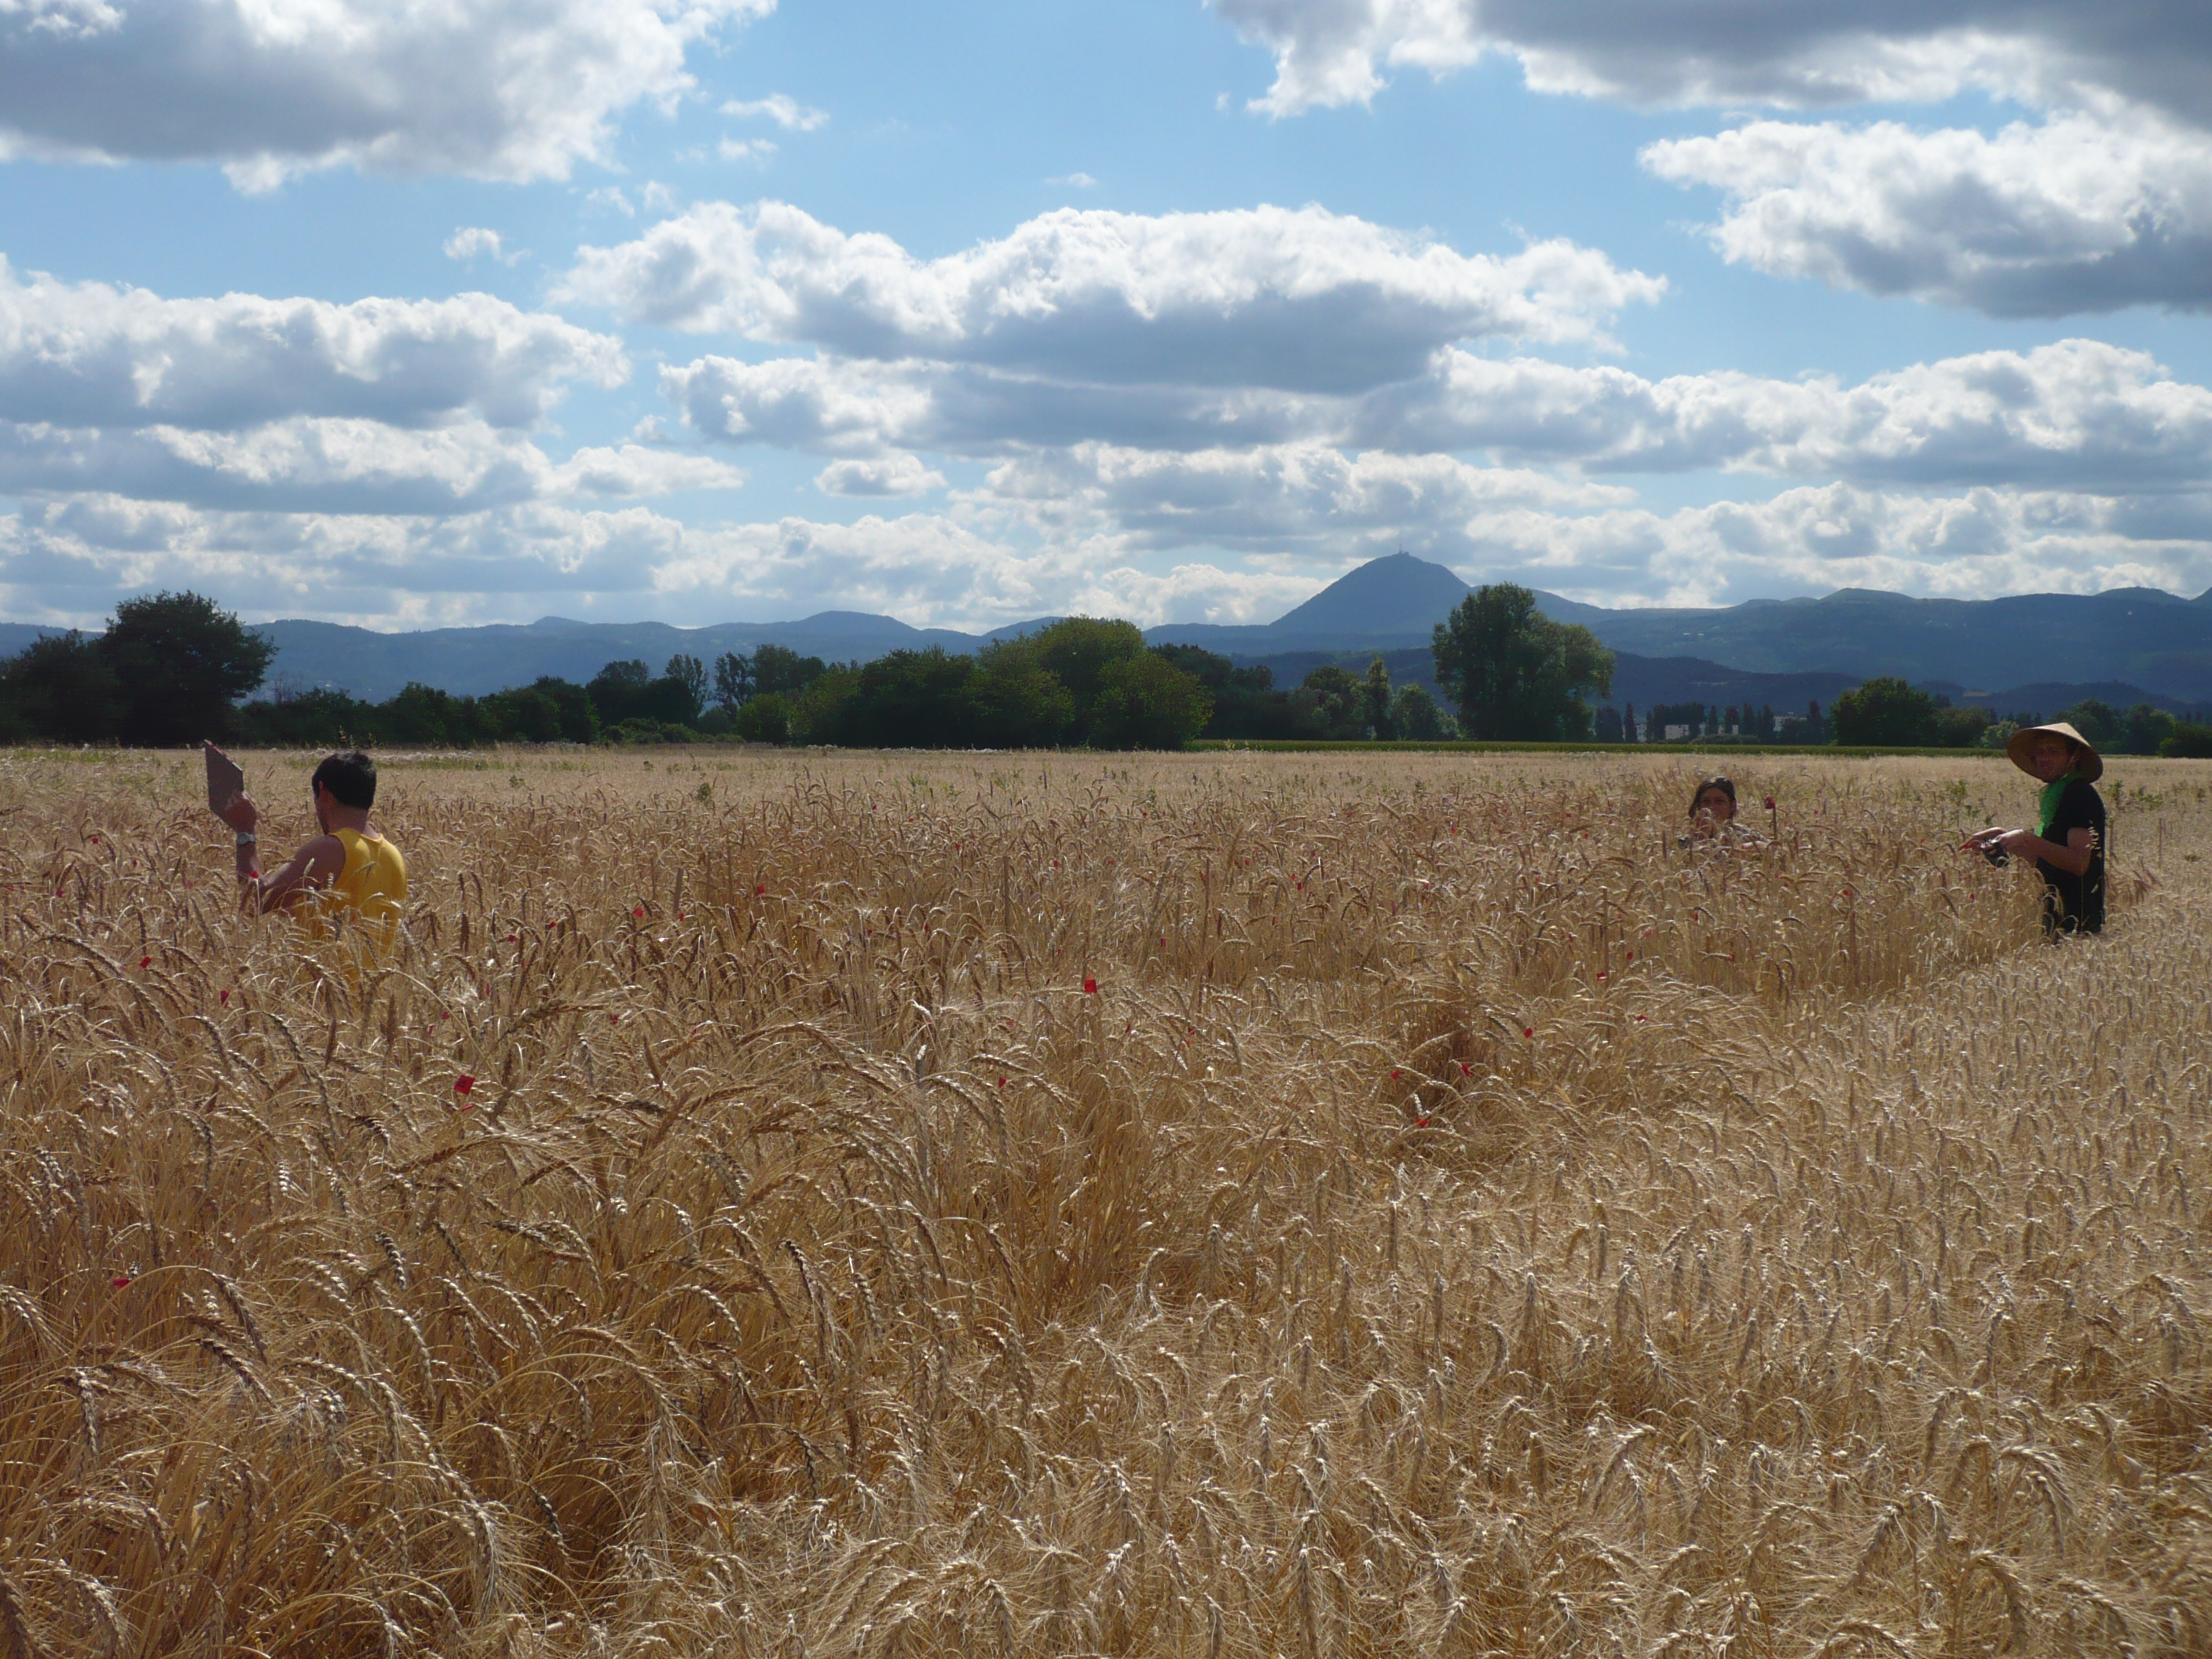
\includegraphics[width=.8\textwidth]{wheat} \\
Wheat trials on farm within our participatory plant breeding programme, summer 2012, Auvergne, France. \\
CC-BY-NC-SA. Pierre Rivière.
\end{center}

\newpage
\pagestyle{plain}


\newpage


% version 0.9.2
\section{Philosophy of \pack}

\subsection{What is \BD?}

Started in 2009, DEAP and ABI teams from INRA Le Moulon developped a data base to store data in a reliable way during research programs dedicated to the study of dynamic management of crop diversity within experimental stations and farmer networks \citep{thomas_gestion_2011}. 

From 2011 to 2013, this data base was migrated to \BDfull~(\BD) and has evolved in a participatory plant breeding program involving INRA Le Moulon and the Réseau Semences Paysannes (RSP) on bread wheat \citep{riviere_methodologie_2014}.

From 2014 to today, farmers organisations' facilitators informed on  their specific needs for their data management, involving other species than bread wheat such as maize, tomatos or trees. Specific developments were performed to fit the farmers organisations' needs. 

\BD~stores information related to (Figure \ref{relation_SL}):
\begin{itemize}
\item network relations between \sl
\item data linked to the \sl~and to the relations between \sl
\end{itemize}

\begin{figure}[H]
\begin{center}
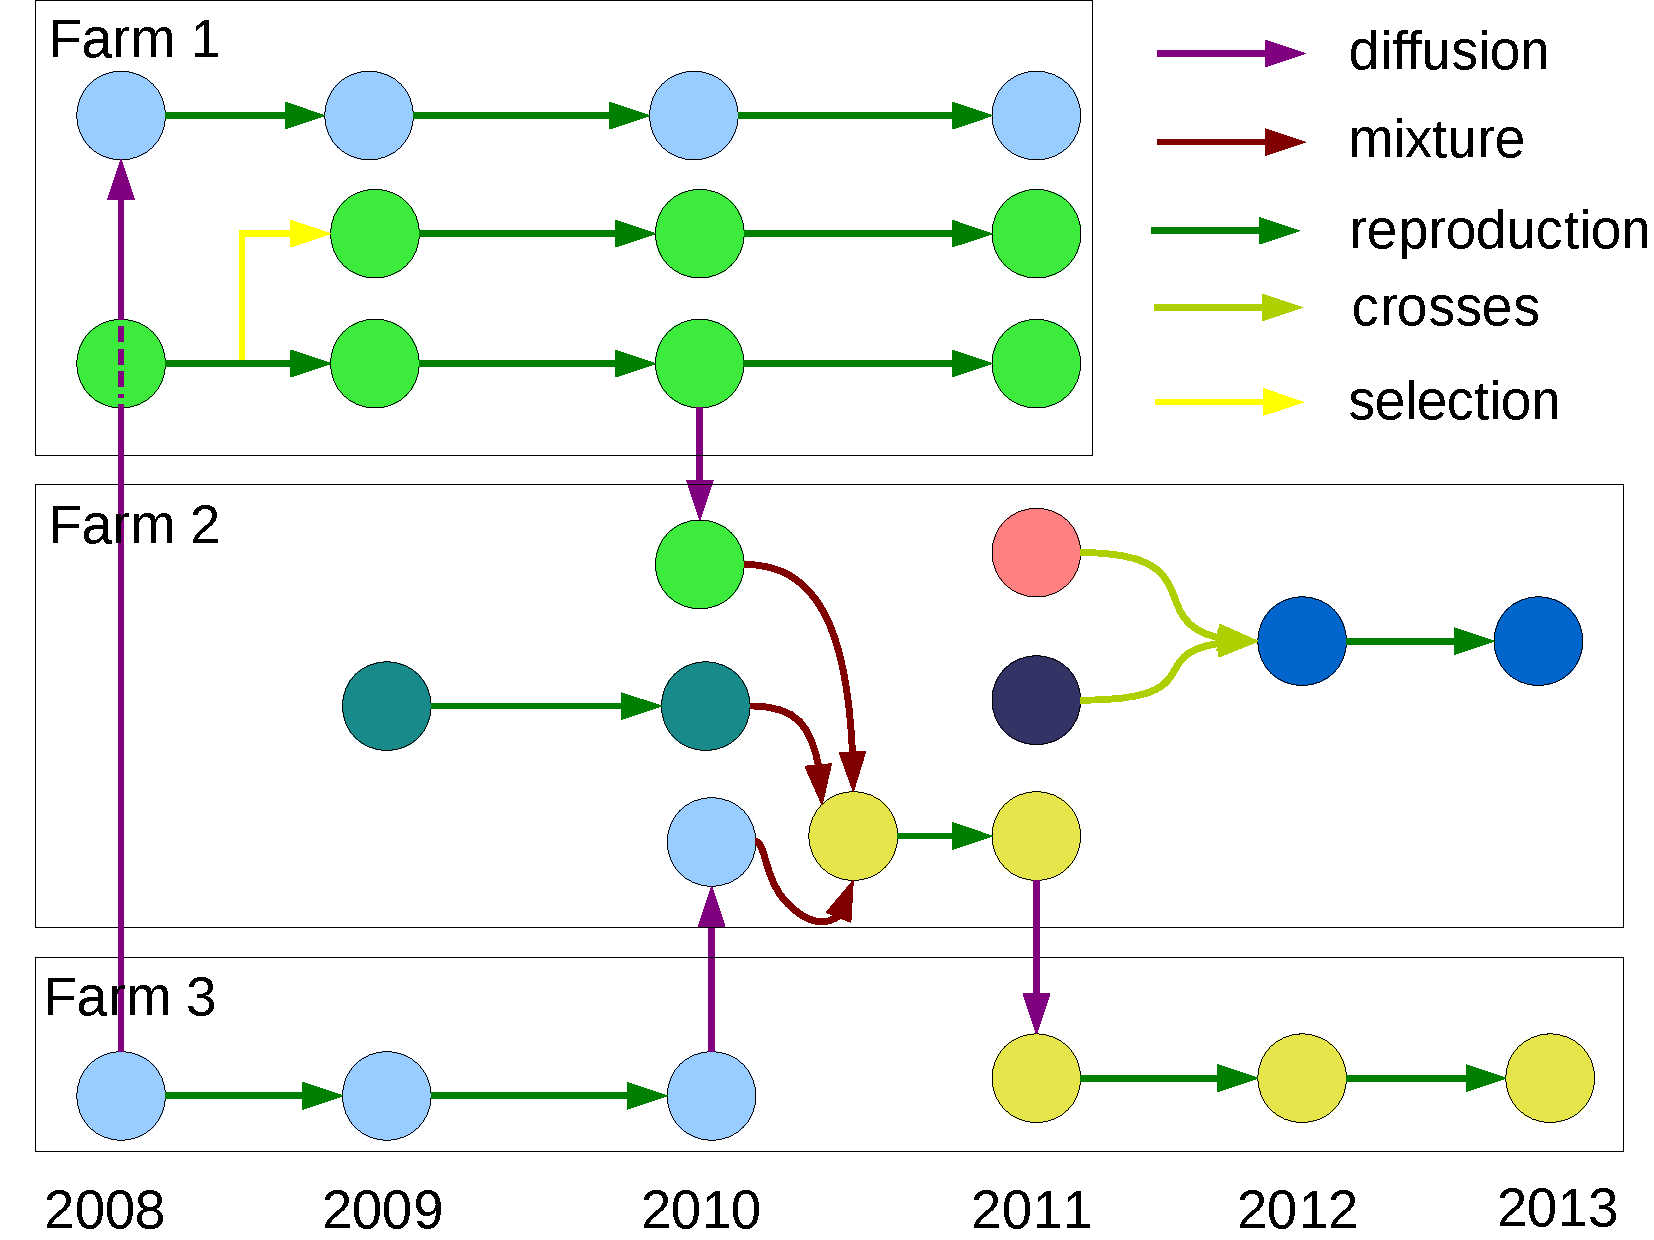
\includegraphics[width=.8\textwidth]{relation_SL_EN}
\caption{
Seed-lots relations in \BD. 
The \sl~are represented by a circle.
The color represents a germplasm (i.e. a variety).
The arrows represent the relations between \sl~(diffusion, mixture, reproduction, crosses and selection).
Data are linked to the \sl~and to the relations between \sl.
}
\label{relation_SL}
\end{center}
\end{figure}

\BD~can be downloaded \href{http://moulon.inra.fr/index.php/en/tranverse-team/atelier-de-bioinformatique/projects/181}{here}.
More information on the history of \BD~and its uses with tutorials can be found on the \href{http://moulon.inra.fr/index.php/en/tranverse-team/atelier-de-bioinformatique/projects/181}{website} \citep{deoliveira_shinemas_2015}.\\

\pack~is an \R~package that analyses outputs from \BD.
It does descriptive analysis, formats data for existing \R~packages to perform statistical analysis as well as compiling results in pdf.


\subsection{Function relations in \pack}

\pack~is divided into three steps (Figure \ref{function_relations}):

\begin{enumerate}
\item Get the data from \BD~with \texttt{get.data}. It is possible to use data in the same format than \texttt{get.data} outputs. This can be done with \texttt{is.get.data.output}. This is useful when the user do not have SHiNeMaS but wish to use the other functions of the package.

You may encrypt the data with \texttt{encrypt.data} or translate it with \texttt{translate.data}.
There are two types of data:
\begin{itemize}
\item network relations between \sl~(section \ref{network})
\item data linked to the \sl~and to the relations between \sl~(section \ref{data})
\end{itemize}

\item From the data,
	\begin{enumerate}
	\item Get descriptive outputs from the data: plots with \texttt{get.ggplot} or tables with \texttt{get.table}
	\item Get statistical outputs by formating the data with \texttt{format.data} in order to use an existing \R~package~(the following package can be used: \listpackformatdata).
	\end{enumerate}
\item Get a pdf that compiles the outputs in a pdf document with \texttt{get.pdf} (section \ref{pdf})
\end{enumerate}


\begin{figure}[H]
\begin{center}
%\begin{tikzpicture}[node distance = 2.5cm, auto]
%    % Place nodes
%    \node [block] (data) {get.data};
%    \node [block, below of=data] (plot) {\texttt{get.ggplot}};
%    \node [block, right of=plot] (table) {\texttt{get.table}};
%	\node [block, left of=plot] (format) {\texttt{format.data}};
%	\node [block, below of=format] (pack) {R package};
%	\node [block, below of=pack, right of=pack] (doc) {\texttt{get.doc}};
%
%    % Draw edges
%    \path [line] (data) -- (plot);
%    \path [line] (data) -- (table);
%    \path [line] (plot) -- (doc);
%    \path [line] (table) -- (doc);
%    \path [line,dashed] (data) -- (format);
%    \path [line,dashed] (format) -- (pack);
%    \path [line,dashed] (pack) -- (doc);
%\end{tikzpicture}
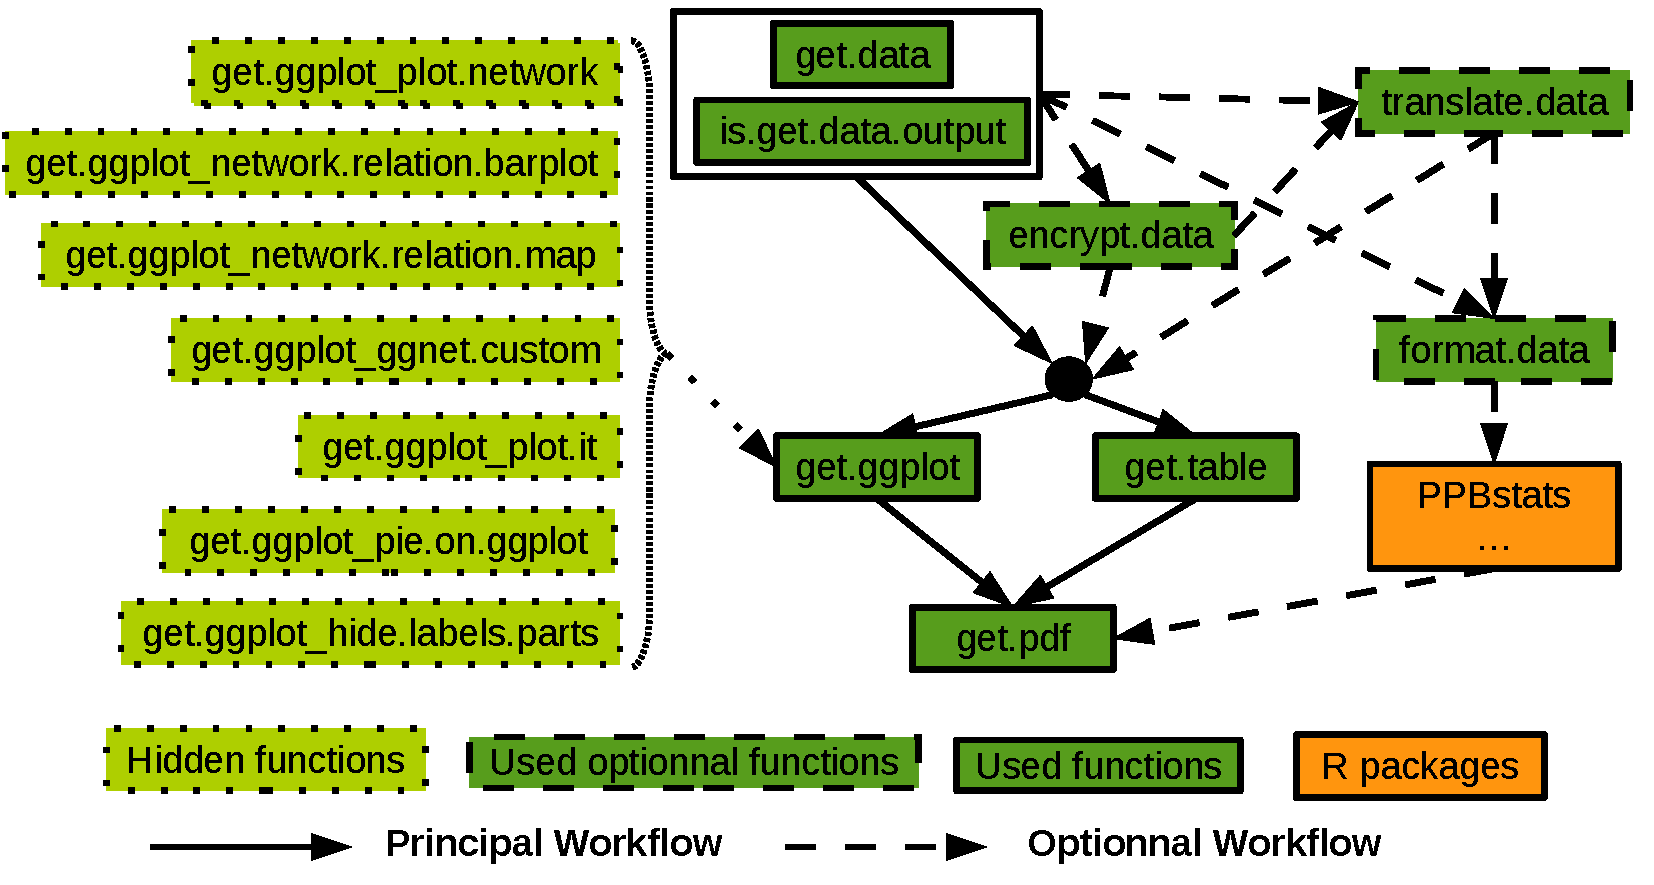
\includegraphics[width=\textwidth]{shinemas2R_function_relations}
\end{center}
\caption{Relations between functions in \pack}
\label{function_relations}
\end{figure}

\texttt{get.ggplot} is based on \texttt{ggplot2} package.
It is therefore easy to customize a plot generated by \texttt{get.ggplot} by adding layers.
More details can be found on the \texttt{ggplot2} documentation website: \url{http://ggplot2.org}.

\subsection{Let’s go!}

To continue, load the package:
\begin{knitrout}
\definecolor{shadecolor}{rgb}{0.969, 0.969, 0.969}\color{fgcolor}\begin{kframe}
\begin{alltt}
\hlkwd{library}\hlstd{(shinemas2R)}
\end{alltt}
\end{kframe}
\end{knitrout}

For an easier visualization in the vignette, all warning messages are not represented (NAs introduced, rows deleted, etc.)

\subsubsection{Test with \BD~installed}

It may be useful to test the \texttt{get.data} function on \BD~directly.
Two options:
\begin{itemize}
\item \BD~is installed on a server you can have access to. 
You need to ask the admin the following information: \texttt{db\_user}, \texttt{db\_host}, \texttt{db\_name}, \texttt{db\_password}. 
Add these information into \texttt{info\_db}, which is needed in the next steps in \texttt{get.data}.
For example: 

\begin{knitrout}
\definecolor{shadecolor}{rgb}{0.969, 0.969, 0.969}\color{fgcolor}\begin{kframe}
\begin{alltt}
\hlstd{info_db} \hlkwb{=} \hlkwd{list}\hlstd{(}
        \hlkwc{db_user} \hlstd{=} \hlstr{"pierre"}\hlstd{,}
        \hlkwc{db_host} \hlstd{=} \hlstr{"127.0.0.1"}\hlstd{,} \hlcom{# localhost}
        \hlkwc{db_name} \hlstd{=} \hlstr{"shinemas_dev"}\hlstd{,}
        \hlkwc{db_password} \hlstd{=} \hlstr{"toto"}
\hlstd{)}
\end{alltt}
\end{kframe}
\end{knitrout}

\item install a demo of \BD~on your computer.
The procedure to do so is explained in appendix \ref{install_shinemas}.

\end{itemize}

As you will use \texttt{get.data}, you should set:
\begin{knitrout}
\definecolor{shadecolor}{rgb}{0.969, 0.969, 0.969}\color{fgcolor}\begin{kframe}
\begin{alltt}
\hlstd{use.get.data} \hlkwb{=} \hlnum{TRUE}
\end{alltt}
\end{kframe}
\end{knitrout}

\subsubsection{Test without \BD~installed}

In this vignette, you can test \pack~without installing \BD.
You do not use the \texttt{get.data} function:
\begin{knitrout}
\definecolor{shadecolor}{rgb}{0.969, 0.969, 0.969}\color{fgcolor}\begin{kframe}
\begin{alltt}
\hlstd{use.get.data} \hlkwb{=} \hlnum{FALSE}
\end{alltt}
\end{kframe}
\end{knitrout}

And you can download the data-sets here : \url{https://www.dropbox.com/sh/u1wrwttbn4mq5l4/AACXqZNtzI6TPUeZ_15eyHz_a?dl=0} and put it in the folder data.

The following code is specific to my computer.
\begin{knitrout}
\definecolor{shadecolor}{rgb}{0.969, 0.969, 0.969}\color{fgcolor}\begin{kframe}
\begin{alltt}
\hlkwd{system}\hlstd{(}\hlstr{"mkdir data"}\hlstd{)}
\hlkwd{system}\hlstd{(}\hlstr{"cp -r /home/pierre/Documents/geek/R-stats/Rdev/R_package_shinemas2R/shinemas2R_data/*RData ./data"}\hlstd{)}
\end{alltt}
\end{kframe}
\end{knitrout}

and then \texttt{load()} it.\\

~\\

In this vignette, there are no examples with \texttt{is.get.data.output}.
Refer to appendix \ref{examples_is_get_data_output} to know the format that must have the data to be used in the other functions of the package (i.e. \texttt{get.ggplot} and \texttt{get.table} followed by \texttt{get.pdf}).






\newpage


% version 0.9.2
\section{Raw information on levels and variables}
\label{raw}

Several information are stored in \BD.
To get information on raw information, levels and variable, you must use the argument \texttt{query.type} in \texttt{get.data}.
The following table summarize the different possibilities:

\begin{center}
\begin{tabular}{ll}
\hline
\texttt{query.type} & type of information present in \BD \\
\hline
"species" & species \\
"variable" & variable \\
"person" & person \\
"year" & year \\
"project" & project \\
"seed.lot" & seed-lots \\
"selection.person" & persons that did intra-varietal mass selection \\
"reproduction.type" & reproduction type \\
"germplasm.type" & germplasm type \\
"germplasm" & germplasm \\
\hline
\end{tabular}
\end{center}

For example,

\begin{knitrout}
\definecolor{shadecolor}{rgb}{0.969, 0.969, 0.969}\color{fgcolor}\begin{kframe}
\begin{alltt}
\hlkwa{if}\hlstd{(use.get.data)\{}
        \hlstd{person} \hlkwb{=} \hlkwd{get.data}\hlstd{(}
                \hlkwc{db_user} \hlstd{= info_db}\hlopt{$}\hlstd{db_user,} \hlkwc{db_host} \hlstd{= info_db}\hlopt{$}\hlstd{db_host,}\hlcom{# db infos}
                \hlkwc{db_name} \hlstd{= info_db}\hlopt{$}\hlstd{db_name,} \hlkwc{db_password} \hlstd{= info_db}\hlopt{$}\hlstd{db_password,} \hlcom{# db infos}
                \hlkwc{query.type} \hlstd{=} \hlstr{"person"} \hlcom{# information on person present in SHiNeMaS}
        \hlstd{)}
\hlstd{\}} \hlkwa{else} \hlstd{\{}
                \hlkwd{load}\hlstd{(}\hlstr{"data/person.RData"}\hlstd{)}
        \hlstd{\}}

\hlstd{person}\hlopt{$}\hlstd{data}
\end{alltt}
\begin{verbatim}
## [1] "JFB" "JSG" "MLN" "OLR"
## attr(,"shinemas2R.object")
## [1] "person"
\end{verbatim}
\end{kframe}
\end{knitrout}



\newpage


% version 0.9.2
\section{Network relations between \sl }
\label{network}

\subsection{Get the data set}

To get the data, use the function \texttt{get.data} with \texttt{query.type = "network"}.

You can set filters to the query with the following argument :

\begin{itemize}
\item \texttt{filter.in} to choose nothing except \texttt{filter.in}
\item \texttt{filter.out} to choose everything except \texttt{filter.out}
\end{itemize}

values of filters can be \texttt{germplasm}, \texttt{germplasm.type}, \texttt{year}, \texttt{person}, \texttt{project}, \texttt{\sl}, \texttt{relation} or \texttt{reproduction.type}.


It is important to choose if you apply the filter on the \texttt{father} or the \texttt{son} of a relation.
This can be done with the argument \texttt{filter.on}.
Possibles values are \texttt{"father"}, \texttt{"son"} or \texttt{"father-son"}.
It is set by default to \texttt{"father-son"}.

It is possible to get the \texttt{Mdist} square matrix with the number of reproductions that separate two seed-lots since their last common diffusion (argument \texttt{Mdist = TRUE}).
Note that a value of 1 means a distance between 
\begin{itemize}
	\item a seed-lot that has been diffused to location A without beeing sown and harvested on location B and
	\item a seed-lot that has been diffused to location B and beeing sown and harvested on location B
\end{itemize}

This square matrix can be compared to a differentiation distance. 
It can be put in relation with genetic $F_{st}$ for example \citep{nei_analysis_1973}\footnote{The \R~package \texttt{adegenet} can be used for that.}.


\begin{knitrout}
\definecolor{shadecolor}{rgb}{0.969, 0.969, 0.969}\color{fgcolor}\begin{kframe}
\begin{alltt}
\hlkwa{if}\hlstd{(use.get.data)\{}
        \hlstd{data_network} \hlkwb{=} \hlkwd{get.data}\hlstd{(}
                \hlkwc{db_user} \hlstd{= info_db}\hlopt{$}\hlstd{db_user,} \hlkwc{db_host} \hlstd{= info_db}\hlopt{$}\hlstd{db_host,} \hlcom{# db infos}
                \hlkwc{db_name} \hlstd{= info_db}\hlopt{$}\hlstd{db_name,} \hlkwc{db_password} \hlstd{= info_db}\hlopt{$}\hlstd{db_password,} \hlcom{# db infos}
                \hlkwc{query.type} \hlstd{=} \hlstr{"network"}\hlstd{,} \hlcom{# network query}
                \hlkwc{filter.on} \hlstd{=} \hlstr{"father-son"}\hlstd{,} \hlcom{# filter on father AND son}
                \hlkwc{Mdist} \hlstd{=} \hlnum{TRUE}
                \hlstd{)}
\hlstd{\}} \hlkwa{else} \hlstd{\{}
        \hlcom{# 1. Query SHiNeMaS ...}
        \hlcom{# Mixtures from replication have been deleted and replaced by reproductions.}
        \hlcom{# 2. Create network matrix ...}
        \hlcom{# 3. Link information to vertex and edges ...}
        \hlcom{# 4. Get network information on seed-lots ...}
        \hlcom{# 5. Get Mdist square matrix ...}

        \hlkwd{load}\hlstd{(}\hlstr{"./data/data_network.RData"}\hlstd{)}
        \hlstd{\}}
\end{alltt}
\end{kframe}
\end{knitrout}

The function returns a list with:
\begin{itemize}
\item the netwok object
\begin{knitrout}
\definecolor{shadecolor}{rgb}{0.969, 0.969, 0.969}\color{fgcolor}\begin{kframe}
\begin{alltt}
\hlstd{n} \hlkwb{=} \hlstd{data_network}\hlopt{$}\hlstd{data}\hlopt{$}\hlstd{network}
\hlstd{n}
\end{alltt}
\begin{verbatim}
##  Network attributes:
##   vertices = 98 
##   directed = TRUE 
##   hyper = FALSE 
##   loops = FALSE 
##   multiple = FALSE 
##   bipartite = FALSE 
##   total edges= 102 
##     missing edges= 0 
##     non-missing edges= 102 
## 
##  Vertex attribute names: 
##     germplasm germplasm.type person sex vertex.names year 
## 
##  Edge attribute names: 
##     generation relation
\end{verbatim}
\end{kframe}
\end{knitrout}

Note you can convert this object to an \texttt{igraph} object.
This may be useful if you like to use the \texttt{igraph} package.
See \url{http://mbojan.github.io/intergraph/} for more information.

\begin{knitrout}
\definecolor{shadecolor}{rgb}{0.969, 0.969, 0.969}\color{fgcolor}\begin{kframe}
\begin{alltt}
\hlstd{n_igraph} \hlkwb{=} \hlstd{intergraph}\hlopt{::}\hlkwd{asIgraph}\hlstd{(n)}
\hlstd{n_igraph}
\end{alltt}
\begin{verbatim}
## IGRAPH D--- 98 102 -- 
## + attr: germplasm (v/c), germplasm.type (v/c), na (v/l),
## | person (v/c), sex (v/c), vertex.names (v/c), year (v/c),
## | generation (e/c), na (e/l), relation (e/c)
## + edges:
##  [1]  7-> 1  1-> 2  7-> 2  2-> 3  1-> 4  5-> 7  6-> 7 12-> 8  1-> 9
## [10]  9->10  1->11 11->12  6->14 13->14 14->15 15->16 16->17 15->18
## [19] 18->19 25->20 20->21 20->22 22->23 13->25 24->25 20->26 30->27
## [28] 20->28 28->29 22->30 37->31 31->32 31->33 33->34 33->35 24->37
## [37] 36->37 31->38 35->39 31->40 40->41 46->42 42->43 13->45 44->45
## [46] 45->46 46->47 42->48 51->49 49->50  6->51 36->51 49->52 49->53
## + ... omitted several edges
\end{verbatim}
\end{kframe}
\end{knitrout}

\item the network.query dataframe coming from the query
\begin{knitrout}
\definecolor{shadecolor}{rgb}{0.969, 0.969, 0.969}\color{fgcolor}\begin{kframe}
\begin{alltt}
\hlkwd{head}\hlstd{(data_network}\hlopt{$}\hlstd{data}\hlopt{$}\hlstd{network.query)}
\end{alltt}
\begin{verbatim}
##   son_species son_project                son son_germplasm
## 1  ble-tendre        DEMO C1#a_JFB_2013_0001            C1
## 2  ble-tendre        DEMO C1#a_JFB_2014_0001            C1
## 3  ble-tendre        DEMO C1#a_JSG_2014_0001            C1
## 4  ble-tendre        DEMO C1#c_JFB_2014_0001            C1
## 5  ble-tendre        DEMO   C1_JFB_2011_0001            C1
## 6  ble-tendre        DEMO   C1_JFB_2011_0001            C1
##   son_person son_year son_germplasm_type son_alt son_long  son_lat
## 1        JFB     2013               <NA>      NA 0.616363 44.20314
## 2        JFB     2014               <NA>      NA 0.616363 44.20314
## 3        JSG     2014               <NA>      NA 3.087025 45.77722
## 4        JFB     2014               <NA>      NA 0.616363 44.20314
## 5        JFB     2011               <NA>      NA 0.616363 44.20314
## 6        JFB     2011               <NA>      NA 0.616363 44.20314
##   son_total_generation_nb son_local_generation_nb
## 1                       1                       1
## 2                       1                       3
## 3                       2                       1
## 4                       1                       5
## 5                       2                       8
## 6                       5                       2
##   son_generation_confidence son_comments father_species
## 1                         1    blablabla     ble-tendre
## 2                         0    blablabla     ble-tendre
## 3                         1    blablabla     ble-tendre
## 4                         1    blablabla     ble-tendre
## 5                         1    blablabla     ble-tendre
## 6                         1    blablabla     ble-tendre
##   father_project                     father father_germplasm
## 1           DEMO           C1_JFB_2012_0001               C1
## 2           DEMO         C1#a_JFB_2013_0001               C1
## 3           DEMO         C1#a_JFB_2014_0001               C1
## 4           DEMO           C1_JFB_2013_0001               C1
## 5           DEMO   Blé-du-Lot_JFB_2010_0001       Blé-du-Lot
## 6           DEMO Rouge-du-Roc_JFB_2010_0001     Rouge-du-Roc
##   father_person father_year father_germplasm_type father_alt
## 1           JFB        2012                  <NA>         NA
## 2           JFB        2013                  <NA>         NA
## 3           JFB        2014                  <NA>         NA
## 4           JFB        2013                  <NA>         NA
## 5           JFB        2010                  <NA>         NA
## 6           JFB        2010                  <NA>         NA
##   father_long father_lat father_total_generation_nb
## 1    0.616363   44.20314                          5
## 2    0.616363   44.20314                          5
## 3    0.616363   44.20314                          2
## 4    0.616363   44.20314                          1
## 5    0.616363   44.20314                          8
## 6    0.616363   44.20314                          6
##   father_local_generation_nb father_generation_confidence
## 1                          6                            0
## 2                          7                            0
## 3                          8                            0
## 4                          4                            0
## 5                          4                            1
## 6                          5                            1
##   father_comments reproduction_id reproduction_method_name is_male
## 1       blablabla             467                     <NA>       X
## 2       blablabla             484                     <NA>       X
## 3       blablabla            <NA>                     <NA>       X
## 4       blablabla             483                     <NA>       X
## 5       blablabla             454                    cross       M
## 6       blablabla             454                    cross       F
##   block selection_id selection_person mixture_id diffusion_id
## 1     1           40              JFB       <NA>         <NA>
## 2     1         <NA>             <NA>       <NA>         <NA>
## 3  <NA>         <NA>             <NA>       <NA>          266
## 4     1           48              JFB       <NA>         <NA>
## 5     1         <NA>             <NA>       <NA>         <NA>
## 6     1         <NA>             <NA>       <NA>         <NA>
##   relation_year_start relation_year_end
## 1                2012              2013
## 2                2013              2014
## 3                <NA>              <NA>
## 4                2013              2014
## 5                2010              2011
## 6                2010              2011
\end{verbatim}
\end{kframe}
\end{knitrout}


\item the network.info matrix with information on relation in the network.
\begin{knitrout}
\definecolor{shadecolor}{rgb}{0.969, 0.969, 0.969}\color{fgcolor}\begin{kframe}
\begin{alltt}
\hlkwd{head}\hlstd{(data_network}\hlopt{$}\hlstd{data}\hlopt{$}\hlstd{network.info)}
\end{alltt}
\begin{verbatim}
##                   sl alt     long      lat diffusion id.diff
## 1 C1#a_JFB_2013_0001  NA 0.616363 44.20314      <NA>    <NA>
## 2 C1#a_JFB_2014_0001  NA 0.616363 44.20314      <NA>    <NA>
## 3 C1#a_JSG_2014_0001  NA 3.087025 45.77722   receive      19
## 4 C1#c_JFB_2014_0001  NA 0.616363 44.20314      <NA>    <NA>
## 5   C1_JFB_2011_0001  NA 0.616363 44.20314      <NA>    <NA>
## 6   C1_JFB_2011_0001  NA 0.616363 44.20314      <NA>    <NA>
##   reproduction mixture selection cross.info germplasm person year
## 1         <NA>    <NA> selection       <NA>        C1    JFB 2013
## 2      harvest    <NA>      <NA>       <NA>        C1    JFB 2014
## 3         <NA>    <NA>      <NA>       <NA>        C1    JSG 2014
## 4         <NA>    <NA> selection       <NA>        C1    JFB 2014
## 5  harvest-sow    <NA>      <NA>       <NA>        C1    JFB 2011
## 6  harvest-sow    <NA>      <NA>       <NA>        C1    JFB 2011
\end{verbatim}
\end{kframe}
\end{knitrout}

\item the \texttt{Mdist} square matrix
\begin{knitrout}
\definecolor{shadecolor}{rgb}{0.969, 0.969, 0.969}\color{fgcolor}\begin{kframe}
\begin{alltt}
\hlkwd{dim}\hlstd{(data_network}\hlopt{$}\hlstd{data}\hlopt{$}\hlstd{Mdist)}
\end{alltt}
\begin{verbatim}
## [1] 98 98
\end{verbatim}
\end{kframe}
\end{knitrout}

\end{itemize}


You may want to fill gaps into your network data set regarding diffusion events (if the information is stored in \BD!).
This may be usefull, regarding a network on one person, to know where seed-lots come from.
To do so, use \texttt{fill.diffusion.gap = TRUE}.

\begin{knitrout}
\definecolor{shadecolor}{rgb}{0.969, 0.969, 0.969}\color{fgcolor}\begin{kframe}
\begin{alltt}
\hlkwa{if}\hlstd{(use.get.data)\{}
        \hlstd{data_network_OLR} \hlkwb{=} \hlkwd{get.data}\hlstd{(}
                \hlkwc{db_user} \hlstd{= info_db}\hlopt{$}\hlstd{db_user,} \hlkwc{db_host} \hlstd{= info_db}\hlopt{$}\hlstd{db_host,} \hlcom{# db infos}
                \hlkwc{db_name} \hlstd{= info_db}\hlopt{$}\hlstd{db_name,} \hlkwc{db_password} \hlstd{= info_db}\hlopt{$}\hlstd{db_password,}  \hlcom{# db infos}
                \hlkwc{query.type} \hlstd{=} \hlstr{"network"}\hlstd{,} \hlcom{# network query}
                \hlkwc{person.in} \hlstd{=} \hlstr{"OLR"}\hlstd{,} \hlcom{# person to keep}
                \hlkwc{filter.on} \hlstd{=} \hlstr{"father-son"} \hlcom{# filter on father AND son}
                \hlstd{)}
\hlstd{\}} \hlkwa{else} \hlstd{\{}
        \hlcom{# 1. Query SHiNeMaS ...}
        \hlcom{# Mixtures from replication have been deleted and replaced by reproductions.}
        \hlcom{# 2. Create network matrix ...}
        \hlcom{# 3. Link information to vertex and edges ...}
        \hlcom{# 4. Get network information on seed-lots ...}

        \hlkwd{load}\hlstd{(}\hlstr{"./data/data_network_OLR.RData"}\hlstd{)}
        \hlstd{\}}
\end{alltt}
\end{kframe}
\end{knitrout}

\begin{knitrout}
\definecolor{shadecolor}{rgb}{0.969, 0.969, 0.969}\color{fgcolor}\begin{kframe}
\begin{alltt}
\hlkwa{if}\hlstd{(use.get.data)\{}
        \hlstd{data_network_OLR_fill_gap} \hlkwb{=} \hlkwd{get.data}\hlstd{(}
                \hlkwc{db_user} \hlstd{= info_db}\hlopt{$}\hlstd{db_user,} \hlkwc{db_host} \hlstd{= info_db}\hlopt{$}\hlstd{db_host,} \hlcom{# db infos}
                \hlkwc{db_name} \hlstd{= info_db}\hlopt{$}\hlstd{db_name,} \hlkwc{db_password} \hlstd{= info_db}\hlopt{$}\hlstd{db_password,} \hlcom{# db infos}
                \hlkwc{query.type} \hlstd{=} \hlstr{"network"}\hlstd{,} \hlcom{# network query}
                \hlkwc{person.in} \hlstd{=} \hlstr{"OLR"}\hlstd{,} \hlcom{# person to keep}
                \hlkwc{filter.on} \hlstd{=} \hlstr{"father-son"}\hlstd{,} \hlcom{# filter on father AND son}
                \hlkwc{fill.diffusion.gap} \hlstd{=} \hlnum{TRUE}
                \hlstd{)}
\hlstd{\}} \hlkwa{else} \hlstd{\{}
        \hlcom{# 1. Query SHiNeMaS ...}
        \hlcom{# Mixtures from replication have been deleted and replaced by reproductions.}
        \hlcom{# 2. Create network matrix ...}
        \hlcom{# 2.1. Fill diffusion gaps ...}
        \hlcom{# 3. Link information to vertex and edges ...}
        \hlcom{# 4. Get network information on seed-lots ...}

        \hlkwd{load}\hlstd{(}\hlstr{"./data/data_network_OLR_fill_gap.RData"}\hlstd{)}
        \hlstd{\}}
\end{alltt}
\end{kframe}
\end{knitrout}

Sometimes, seed-lots are replicated and then mixted.
This can be seen as 'false' mixture compared to 'real' mixture where the germplasm father and son are different.
In order to take this into account in the analysis of the network, it can be useful to delete the 'false' mixture and declare it as a reproduction.
This can be done with the argument \texttt{mixrep\_to\_repro} which tranform the mixtures of replications into reproductions, i.e. the network keeps only 'real' mixtures (i.e. different germplasm for father and son) and correct the information regarding what have been harvested and sown after as the mixture disappear. 
The value of \texttt{mixrep\_to\_repro} is \texttt{TRUE} by default.


\subsection{Get the ggplots}

Once, you have got the data, you can create plots with the function \texttt{get.ggplot}.

\begin{knitrout}
\definecolor{shadecolor}{rgb}{0.969, 0.969, 0.969}\color{fgcolor}\begin{kframe}
\begin{alltt}
\hlstd{default_network_ggplot} \hlkwb{=} \hlkwd{get.ggplot}\hlstd{(data_network)}
\end{alltt}


{\ttfamily\noindent\itshape\color{messagecolor}{\#\# As ggplot.type is NULL, ggplot.type is set to network-network, network-reproduction-sown, network-reproduction-harvested, network-reproduction-positive-inter-selected, network-reproduction-positive-inter-selected, network-reproduction-negative-inter-selected, network-reproduction-crossed, network-diffusion-sent, network-diffusion-received, network-diffusion-relation, network-mixture-real, network-mixture-rep, network-mixture-all, network-positive-intra-selected\\\#\# As ggplot.display is NULL, ggplot.display is set to c("{}barplot"{}, "{}map"{}). Note that for ggplot.type == "{}network-diffusion-relation"{}, ggplot.display is set to "{}map"{} \\\#\# As x.axis and in.col are NULL, all the combinaisons of x.axis and in.col are done for barplot.}}\begin{verbatim}
## [1] "A METTRE A JOUR QUAND ON AURA EVENT YEAR"
## [1] "A METTRE A JOUR QUAND ON AURA EVENT YEAR"
\end{verbatim}
\end{kframe}
\end{knitrout}

By default, all the possible plots or maps are done.

\begin{knitrout}
\definecolor{shadecolor}{rgb}{0.969, 0.969, 0.969}\color{fgcolor}\begin{kframe}
\begin{alltt}
\hlkwd{names}\hlstd{(default_network_ggplot)}
\end{alltt}
\begin{verbatim}
##  [1] "network-network"                             
##  [2] "network-reproduction-sown"                   
##  [3] "network-reproduction-harvested"              
##  [4] "network-reproduction-positive-inter-selected"
##  [5] "network-reproduction-negative-inter-selected"
##  [6] "network-diffusion-sent"                      
##  [7] "network-diffusion-received"                  
##  [8] "network-diffusion-relation"                  
##  [9] "network-mixture-real"                        
## [10] "network-mixture-rep"                         
## [11] "network-mixture-all"                         
## [12] "network-positive-intra-selected"             
## [13] "network-reproduction-crossed"
\end{verbatim}
\end{kframe}
\end{knitrout}

It is possible to get only one plot by choosing one of the above names with the argument \texttt{ggplot.type}.
Each \texttt{ggplot.type} with default and custom arguments are explained in the following sub-sections.

\subsubsection{\texttt{ggplot.type = "network-network"}}

\paragraph{Default arguments}

By default, the following network is displayed:

\begin{knitrout}
\definecolor{shadecolor}{rgb}{0.969, 0.969, 0.969}\color{fgcolor}\begin{kframe}
\begin{alltt}
\hlstd{p_net_C1} \hlkwb{=} \hlstd{default_network_ggplot}\hlopt{$}\hlstr{"network-network"}
\hlstd{p_net_C1}
\end{alltt}
\end{kframe}

{\centering 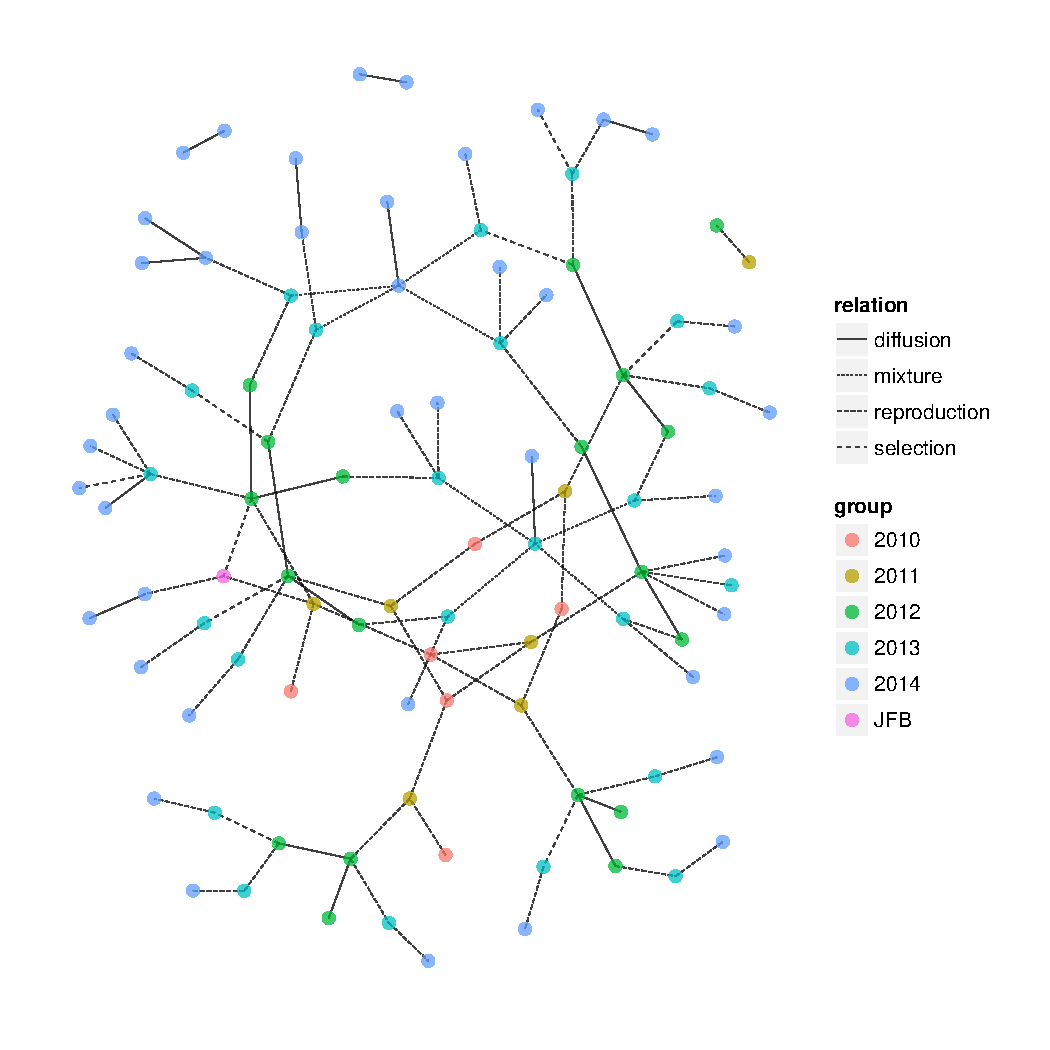
\includegraphics[width=\maxwidth]{figures/shinemas2R_unnamed-chunk-26-1} 

}



\end{knitrout}


Regarding the argument \texttt{fill.diffusion.gap} in the function \texttt{get.data}:

\begin{knitrout}
\definecolor{shadecolor}{rgb}{0.969, 0.969, 0.969}\color{fgcolor}\begin{kframe}
\begin{alltt}
\hlstd{p_OLR} \hlkwb{=} \hlkwd{get.ggplot}\hlstd{(}
        \hlstd{data_network_OLR,}
        \hlkwc{ggplot.type} \hlstd{=} \hlstr{"network-network"}\hlstd{,}
        \hlkwc{vertex.color} \hlstd{=} \hlstr{"person"}
        \hlstd{)}
\hlstd{p_OLR} \hlkwb{=} \hlstd{p_OLR}\hlopt{$}\hlstd{`network-network`}

\hlstd{p_OLR_fill_gap} \hlkwb{=} \hlkwd{get.ggplot}\hlstd{(}
        \hlstd{data_network_OLR_fill_gap,}
        \hlkwc{ggplot.type} \hlstd{=} \hlstr{"network-network"}\hlstd{,}
        \hlkwc{vertex.color} \hlstd{=} \hlstr{"person"}
        \hlstd{)}
\hlstd{p_OLR_fill_gap} \hlkwb{=} \hlstd{p_OLR_fill_gap}\hlopt{$}\hlstd{`network-network`}
\end{alltt}
\end{kframe}
\end{knitrout}

We can see that extra information are added to know from where the seed-lots come from.

\begin{center}
\begin{tabular}{cc}
\texttt{p\_OLR} & \texttt{p\_OLR\_fill\_OLR} \\
\begin{knitrout}
\definecolor{shadecolor}{rgb}{0.969, 0.969, 0.969}\color{fgcolor}

{\centering 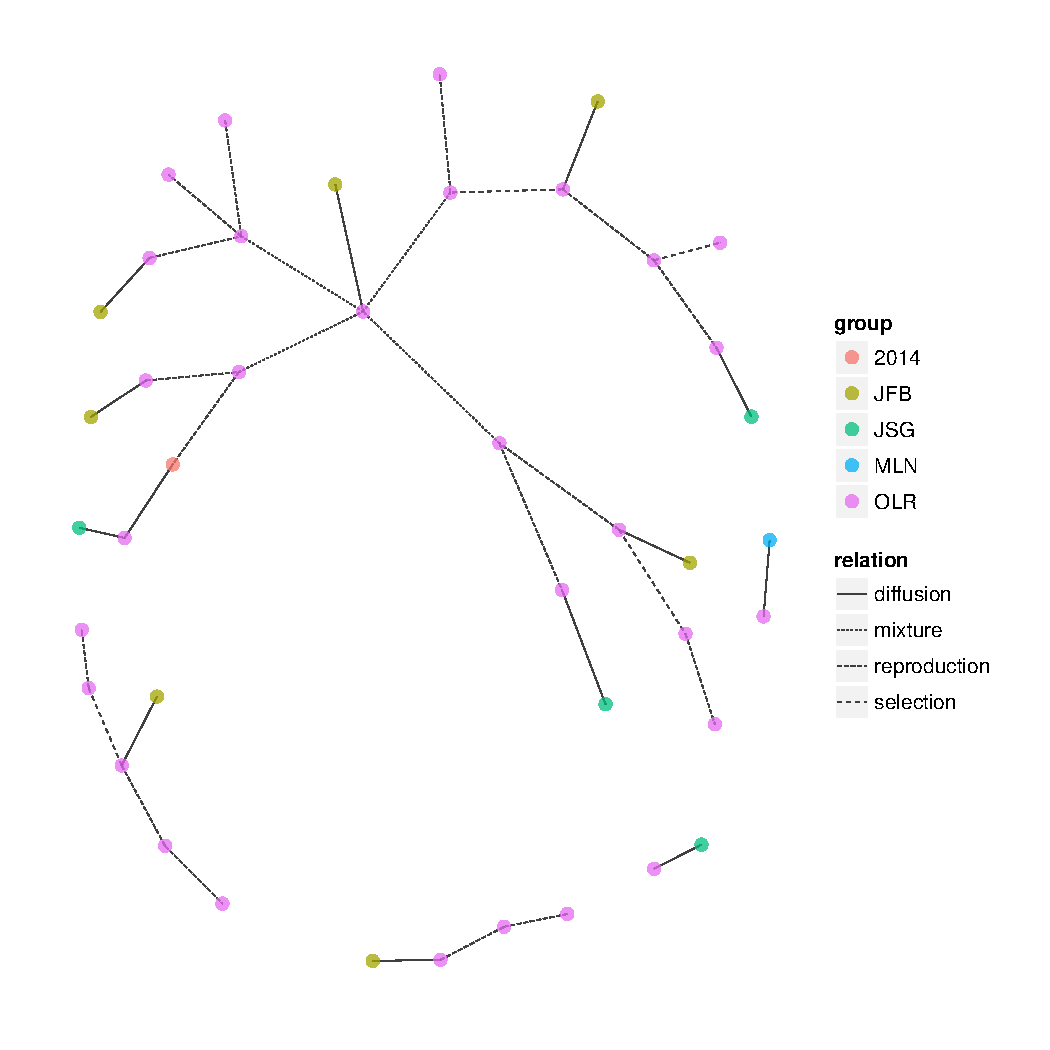
\includegraphics[width=.5\textwidth]{figures/shinemas2R_unnamed-chunk-28-1} 

}



\end{knitrout}
&
\begin{knitrout}
\definecolor{shadecolor}{rgb}{0.969, 0.969, 0.969}\color{fgcolor}

{\centering 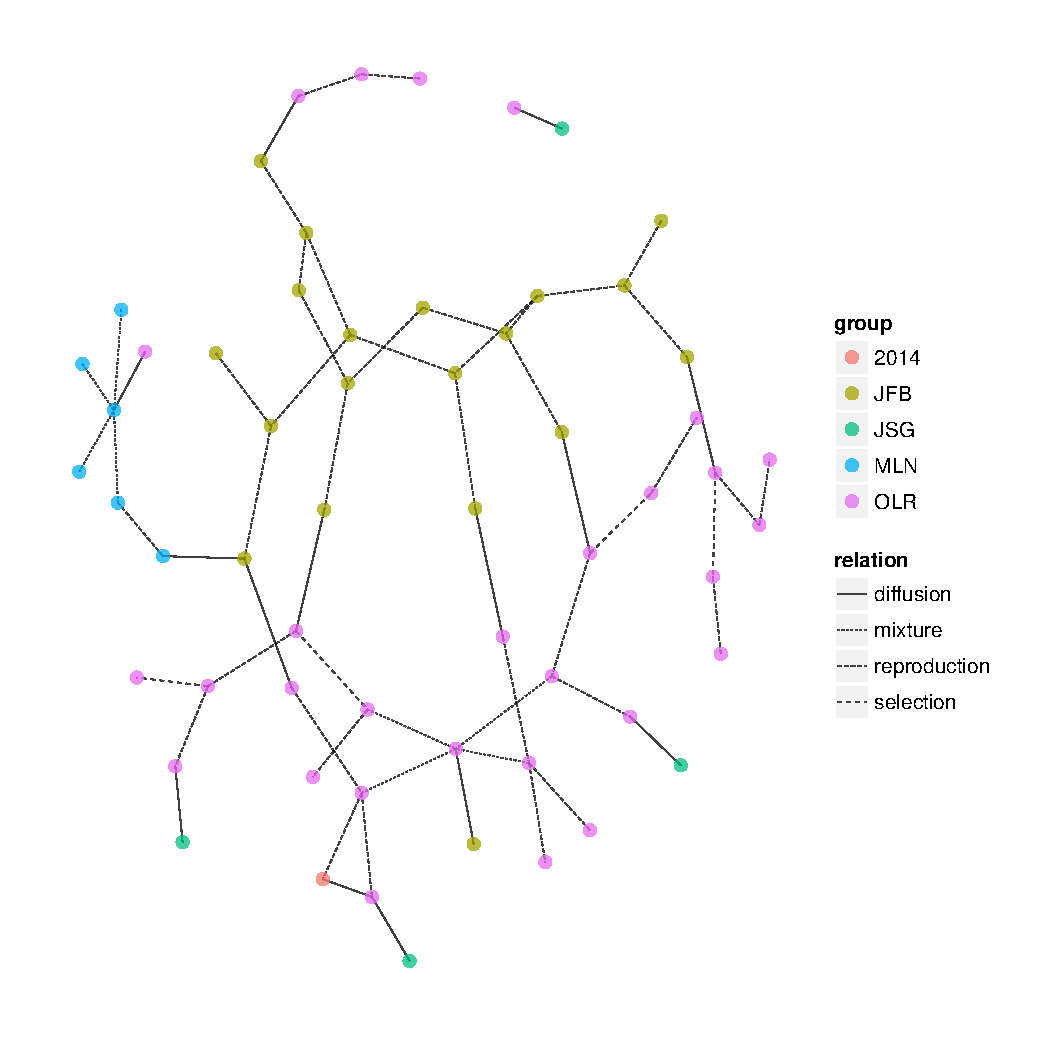
\includegraphics[width=.5\textwidth]{figures/shinemas2R_unnamed-chunk-29-1} 

}



\end{knitrout}
\\
\end{tabular}
\end{center}



\paragraph{Custom arguments}

It is possible to tune the following arguments (Table \ref{custom.network}):


\begin{center}
\begin{table}[H]
\begin{tabular}{ p{.2\textwidth} p{.15\textwidth} p{.6\textwidth} }
\hline
\texttt{argument} & \texttt{default value} & description \\
\hline

\texttt{vertex.size} & \texttt{3} &  size of the vertex \\

\texttt{vertex.color} & \texttt{"year"} & color of the vertex. 
It can be chosen according to  \texttt{"person"}, \texttt{"germplasm"} or \texttt{"year"}. 
If \texttt{NULL}, it is in black. \\

\texttt{organise.sl} & \texttt{FALSE} & organize seed-lots for an easier visualization \\

\texttt{hide.labels.parts} & \texttt{"all"} & parts of the label hidden: \texttt{"germplasm"}, \texttt{"person"}, \texttt{"year"}, \texttt{"person:germplasm"}, \texttt{"year:germplasm"}, \texttt{"person:year"}, \texttt{"all"}. 
\texttt{"all"} means that no label is dispayed. 
If \texttt{NULL} labels are displayed. Labels are based on seed-lots names under the form \texttt{germplasm\_year\_person\_digit}.
For easier visualisation, digit is never display unless you choose \texttt{NULL}.
\\

\texttt{labels.sex} & \texttt{TRUE} & if \texttt{TRUE}, display the sex of the seed-lot if it has been used in a cross. Nothing is displayed if hide.labels.parts = \texttt{"all"}. \\

\texttt{labels.generation} & \texttt{TRUE} & if TRUE, display generation for each reproduction. \\

\texttt{labels.size} & \texttt{3} & size of the labels \\
\hline
\end{tabular}
\caption{Possible arguments to custom arguments regarding network.}
\label{custom.network}
\end{table}
\end{center}


For example,

\begin{knitrout}
\definecolor{shadecolor}{rgb}{0.969, 0.969, 0.969}\color{fgcolor}\begin{kframe}
\begin{alltt}
\hlkwd{get.ggplot}\hlstd{(}
        \hlstd{data_network,}
        \hlkwc{ggplot.type} \hlstd{=} \hlstr{"network-network"}\hlstd{,}
        \hlkwc{organise.sl} \hlstd{=} \hlnum{TRUE}\hlstd{,}
        \hlkwc{hide.labels.parts} \hlstd{=} \hlstr{"year:germplasm"}\hlstd{,}
        \hlkwc{vertex.color} \hlstd{=} \hlstr{"year"}
        \hlstd{)}
\end{alltt}
\begin{verbatim}
## $`network-network`
\end{verbatim}
\end{kframe}


{\centering 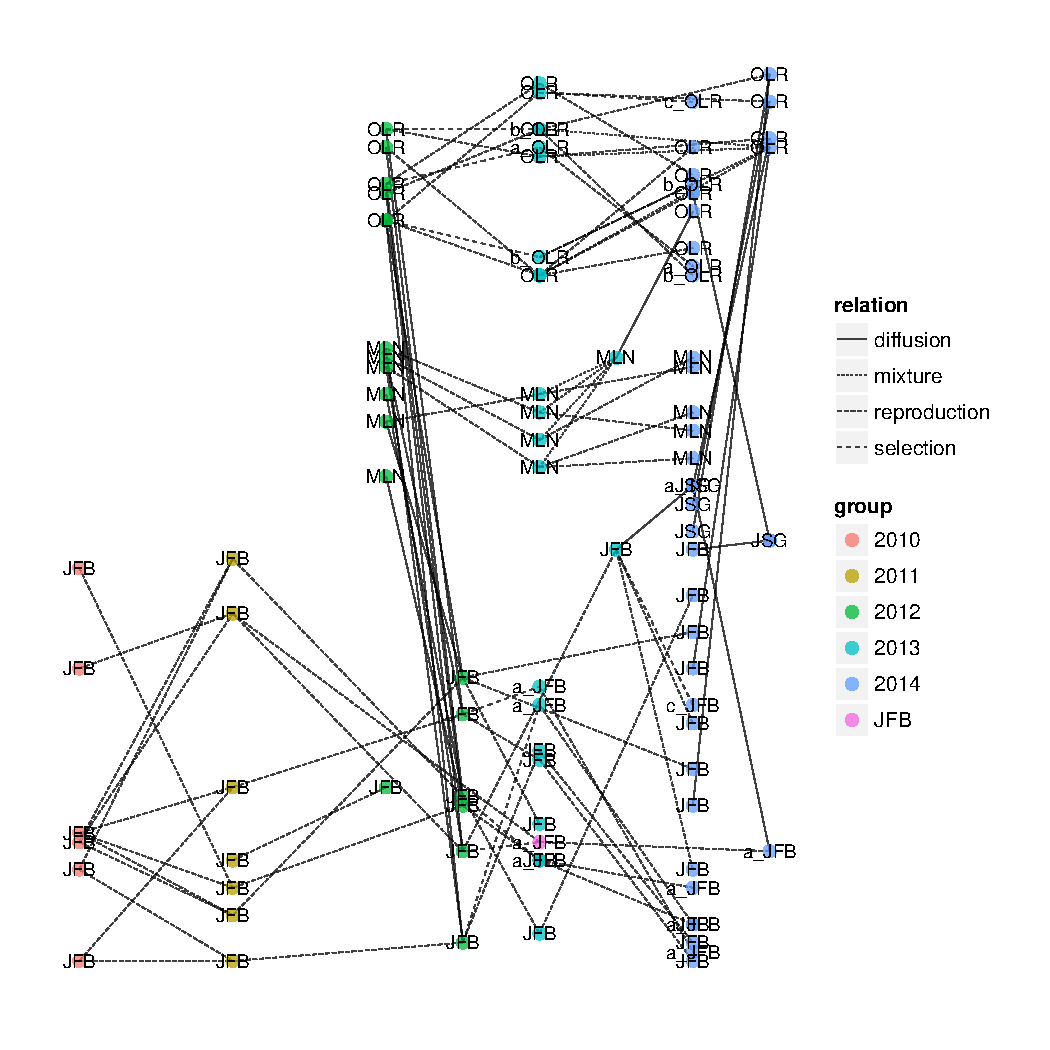
\includegraphics[width=\maxwidth]{figures/shinemas2R_unnamed-chunk-30-1} 

}



\end{knitrout}

\subsubsection{\texttt{ggplot.type = "network-reproduction-harvested"}}


\texttt{ggplot.type = "network-reproduction-harvested"} corresponds to seed-lots that have been harvested after a reproduction.


Two plots are possible regarding \texttt{ggplot.display}.

\begin{center}
\begin{tabular}{ p{.2\textwidth} p{.15\textwidth} p{.6\textwidth} }
\hline
argument & default value & description \\
\hline
\texttt{ggplot.display} & \texttt{NULL} & \texttt{"barplot"} or  \texttt{"map"}.
It can be a vector of several elements i.e. \texttt{c("barplot", "map")}. 
\texttt{NULL} by default: both are done. \\
\hline
\end{tabular}
\end{center}


\paragraph{\texttt{ggplot.display = barplot}}

For \texttt{ggplot.display = "barplot"}, you may chose what you want in the x axis (\texttt{x.axis} argument) and in color (\texttt{in.col} argument).
The possible values for \texttt{x.axis} and \texttt{in.col} are: \texttt{germplasm}, \texttt{year}, \texttt{person}.
By default all combinaisons of \texttt{x.axis} and \texttt{in.col} are done with default argument settings.
The name of the plot is under the form \texttt{x.axis}-\texttt{in.col}.


\begin{itemize}

\item Default arguments

\begin{knitrout}
\definecolor{shadecolor}{rgb}{0.969, 0.969, 0.969}\color{fgcolor}\begin{kframe}
\begin{alltt}
\hlstd{p_slh} \hlkwb{=} \hlstd{default_network_ggplot}\hlopt{$}\hlstd{`network-reproduction-harvested`}\hlopt{$}\hlstd{barplot}
\hlstd{p1_slh} \hlkwb{=} \hlstd{p_slh}\hlopt{$}\hlstd{`germplasm-year`}\hlopt{$}\hlstd{`x.axis-1|in.col-1`}
\hlstd{p2_slh} \hlkwb{=} \hlstd{p_slh}\hlopt{$}\hlstd{`germplasm-person`}\hlopt{$}\hlstd{`x.axis-1|in.col-1`}
\hlstd{p3_slh} \hlkwb{=} \hlstd{p_slh}\hlopt{$}\hlstd{`person-year`}\hlopt{$}\hlstd{`x.axis-1|in.col-1`}
\hlstd{p4_slh} \hlkwb{=} \hlstd{p_slh}\hlopt{$}\hlstd{`person-germplasm`}\hlopt{$}\hlstd{`x.axis-1|in.col-1`}
\hlstd{p5_slh} \hlkwb{=} \hlstd{p_slh}\hlopt{$}\hlstd{`year-person`}\hlopt{$}\hlstd{`x.axis-1|in.col-1`}
\hlstd{p6_slh} \hlkwb{=} \hlstd{p_slh}\hlopt{$}\hlstd{`year-germplasm`}\hlopt{$}\hlstd{`x.axis-1|in.col-1`}
\end{alltt}
\end{kframe}
\end{knitrout}

with

\begin{center}
\begin{tabular}{ccc}
\hline
plot & \texttt{x.axis} & \texttt{in.col} \\
\hline
\texttt{p1\_slh} & \texttt{"germplasm"} & \texttt{"year"} \\
\texttt{p2\_slh} & \texttt{"germplasm"} & \texttt{"person"} \\
\texttt{p3\_slh} & \texttt{"person"} & \texttt{"year"} \\
\texttt{p4\_slh} & \texttt{"person"} & \texttt{"germplasm"} \\
\texttt{p5\_slh} & \texttt{"year"} & \texttt{"person"} \\
\texttt{p6\_slh} & \texttt{"year"} & \texttt{"germplasm"} \\
\hline
\end{tabular}
\end{center}


\begin{center}
\begin{tabular}{cc}
\texttt{p1\_slh} & \texttt{p2\_slh} \\
\begin{knitrout}
\definecolor{shadecolor}{rgb}{0.969, 0.969, 0.969}\color{fgcolor}

{\centering 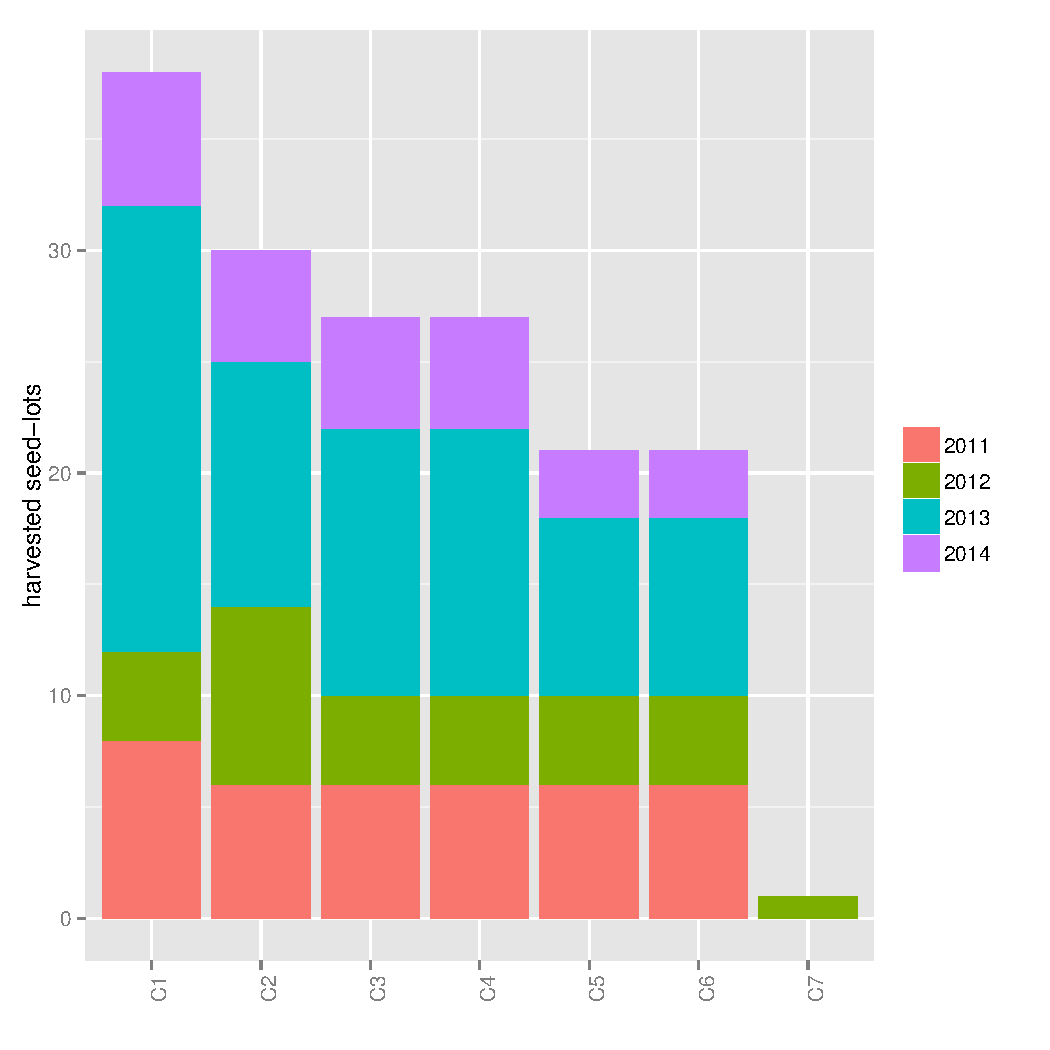
\includegraphics[width=.4\textwidth]{figures/shinemas2R_unnamed-chunk-32-1} 

}



\end{knitrout}
&
\begin{knitrout}
\definecolor{shadecolor}{rgb}{0.969, 0.969, 0.969}\color{fgcolor}

{\centering 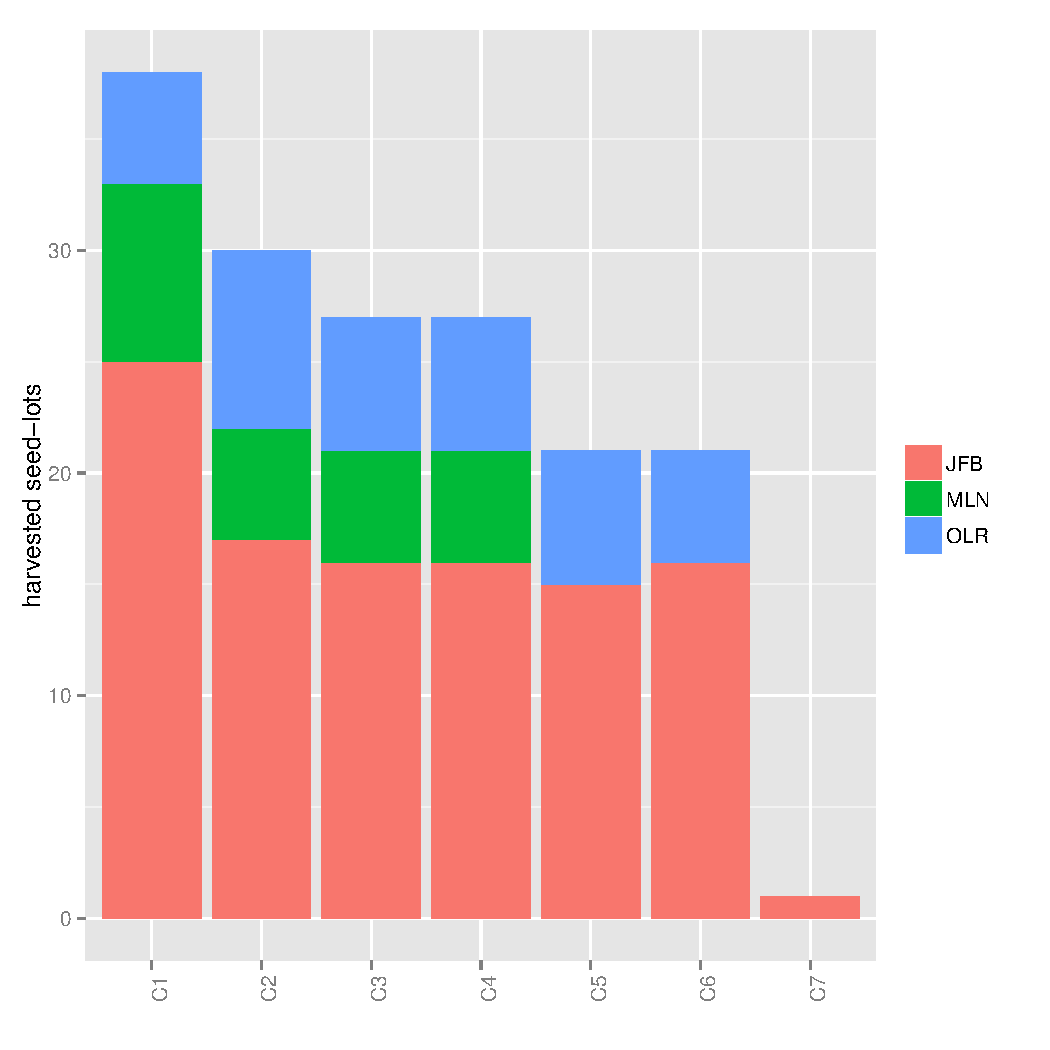
\includegraphics[width=.4\textwidth]{figures/shinemas2R_unnamed-chunk-33-1} 

}



\end{knitrout}
\\
\texttt{p3\_slh} & \texttt{p4\_slh} \\
\begin{knitrout}
\definecolor{shadecolor}{rgb}{0.969, 0.969, 0.969}\color{fgcolor}

{\centering 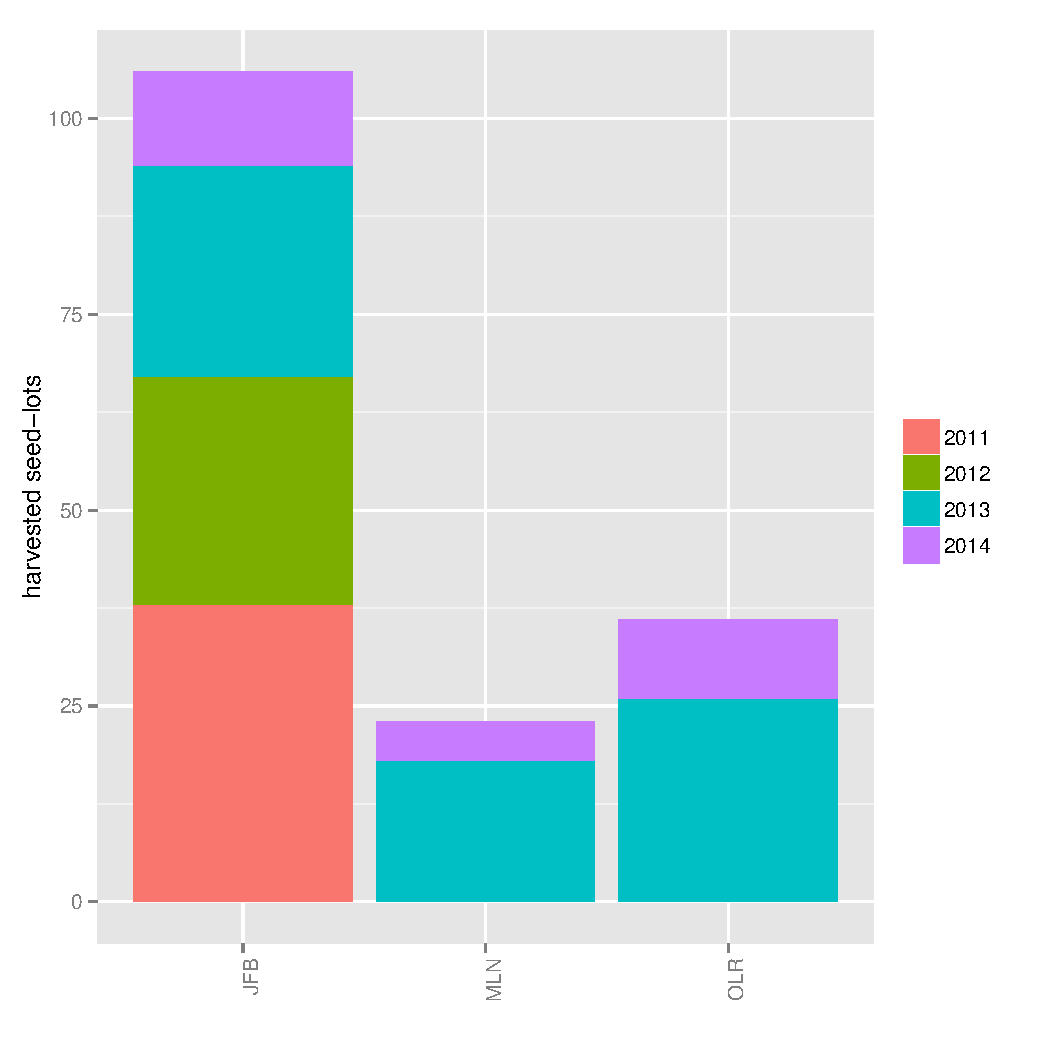
\includegraphics[width=.4\textwidth]{figures/shinemas2R_unnamed-chunk-34-1} 

}



\end{knitrout}
&
\begin{knitrout}
\definecolor{shadecolor}{rgb}{0.969, 0.969, 0.969}\color{fgcolor}

{\centering 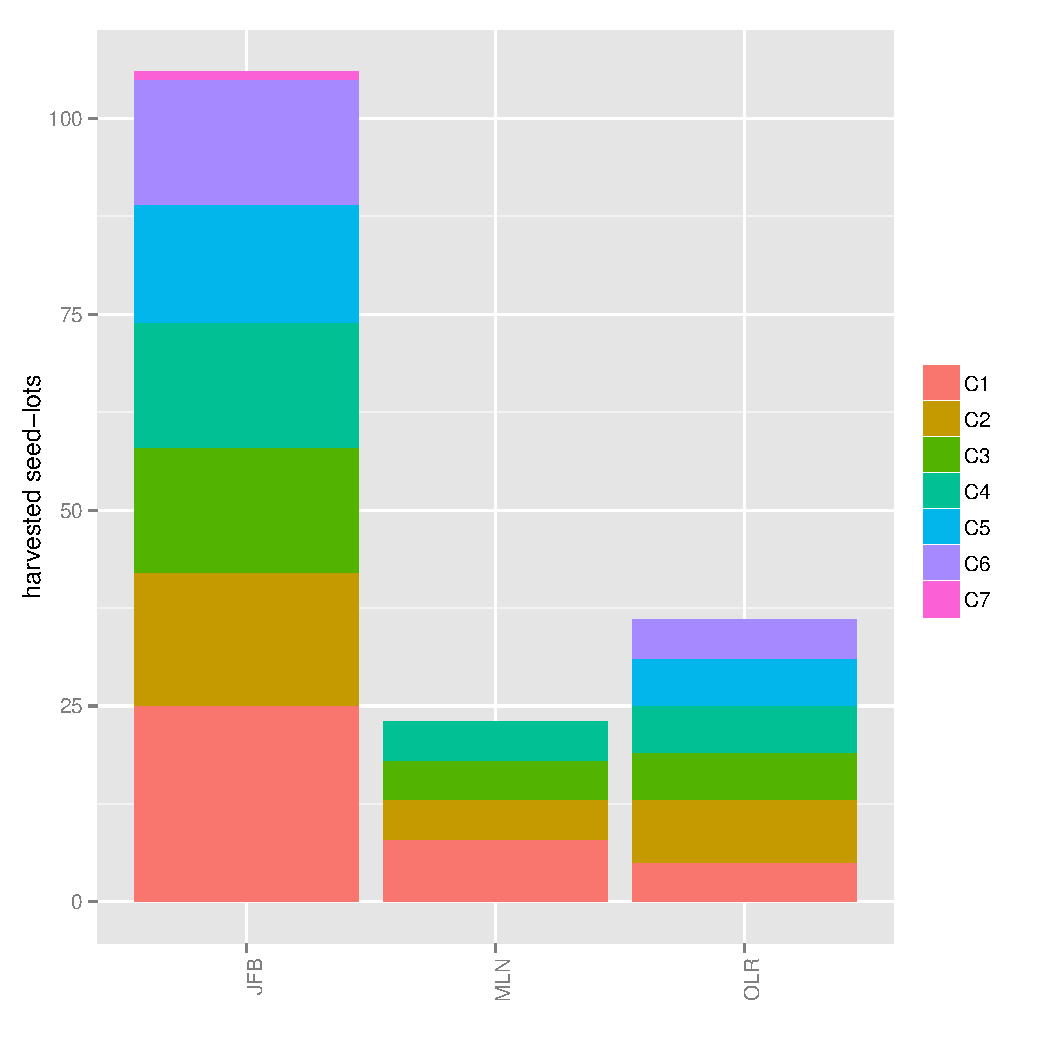
\includegraphics[width=.4\textwidth]{figures/shinemas2R_unnamed-chunk-35-1} 

}



\end{knitrout}
\\
\texttt{p5\_slh} & \texttt{p6\_slh} \\
\begin{knitrout}
\definecolor{shadecolor}{rgb}{0.969, 0.969, 0.969}\color{fgcolor}

{\centering 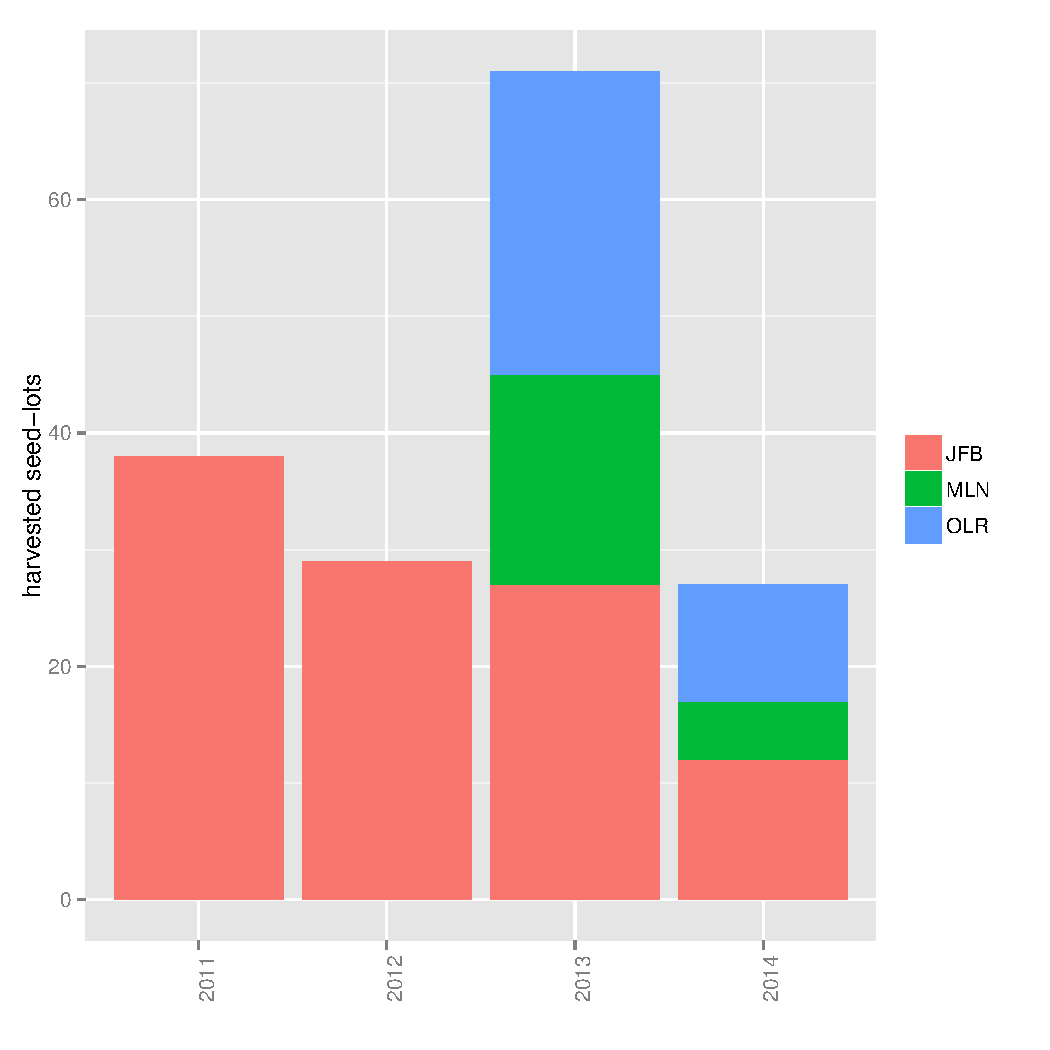
\includegraphics[width=.4\textwidth]{figures/shinemas2R_unnamed-chunk-36-1} 

}



\end{knitrout}
&
\begin{knitrout}
\definecolor{shadecolor}{rgb}{0.969, 0.969, 0.969}\color{fgcolor}

{\centering 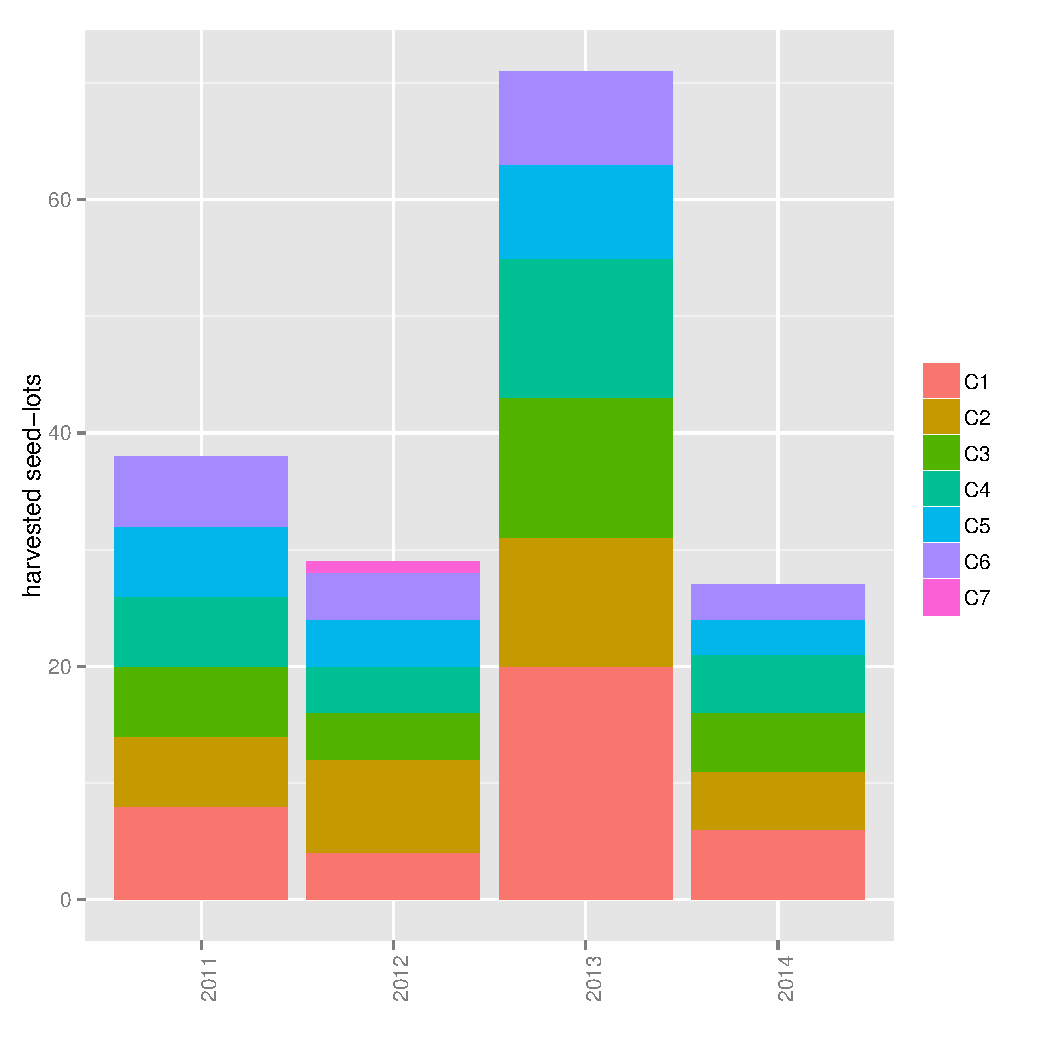
\includegraphics[width=.4\textwidth]{figures/shinemas2R_unnamed-chunk-37-1} 

}



\end{knitrout}
\\
\end{tabular}
\end{center}

\item Custom arguments

It is possible to tune the following arguments:

\begin{center}
\begin{table}[H]
\begin{tabular}{ p{.35\textwidth} p{.15\textwidth} p{.45\textwidth} }
\hline
argument & default value & description \\
\hline

\texttt{x.axis} & \texttt{NULL} & factor displayed on the x.axis of a plot: \texttt{"germplasm"}, \texttt{"year"} or \texttt{"person"} referring to the attributes of a seed-lots. If NULL, all the combinaison are done for \texttt{x.axis} and \texttt{in.col}. \\
\hline

\texttt{in.col} & \texttt{NULL} & display in color of a plot: \texttt{"germplasm"}, \texttt{"year"} or \texttt{"person"} referring to the attributes of a seed-lots. If \texttt{NULL}, \texttt{in.col} is not displayed. \\
\hline

\texttt{nb\_parameters\_per\_plot\_x.axis} & \texttt{NULL} & the number of parameters per plot on \texttt{x.axis} argument \\
\hline

\texttt{nb\_parameters\_per\_plot\_in.col} & \texttt{NULL} & the number of parameters per plot for \texttt{in.col} argument \\

\hline
\end{tabular}
\caption{Possible arguments to custom arguments regarding barplot.}
\label{custom.barplot}
\end{table}
\end{center}



For example, for a given \texttt{x.axis} and a given \texttt{in.col}:
\begin{knitrout}
\definecolor{shadecolor}{rgb}{0.969, 0.969, 0.969}\color{fgcolor}\begin{kframe}
\begin{alltt}
\hlstd{p_slh} \hlkwb{=} \hlkwd{get.ggplot}\hlstd{(}
        \hlstd{data_network,}
        \hlkwc{ggplot.type} \hlstd{=} \hlstr{"network-reproduction-harvested"}\hlstd{,}
        \hlkwc{ggplot.display} \hlstd{=} \hlstr{"barplot"}\hlstd{,}
        \hlkwc{x.axis} \hlstd{=} \hlstr{"person"}\hlstd{,}
        \hlkwc{in.col} \hlstd{=} \hlstr{"year"}
        \hlstd{)}
\end{alltt}
\end{kframe}
\end{knitrout}

It can be useful to separate the plot in several plots regarding \texttt{x.axis}:
\begin{knitrout}
\definecolor{shadecolor}{rgb}{0.969, 0.969, 0.969}\color{fgcolor}\begin{kframe}
\begin{alltt}
\hlstd{p1_slh} \hlkwb{=} \hlkwd{get.ggplot}\hlstd{(}
        \hlstd{data_network,}
        \hlkwc{ggplot.type} \hlstd{=} \hlstr{"network-reproduction-harvested"}\hlstd{,}
        \hlkwc{ggplot.display} \hlstd{=} \hlstr{"barplot"}\hlstd{,}
        \hlkwc{x.axis} \hlstd{=} \hlstr{"person"}\hlstd{,}
        \hlkwc{in.col} \hlstd{=} \hlstr{"year"}\hlstd{,}
        \hlkwc{nb_parameters_per_plot_x.axis} \hlstd{=} \hlnum{2}
        \hlstd{)}

\hlstd{p11_slh} \hlkwb{=} \hlstd{p1_slh}\hlopt{$}\hlstd{`network-reproduction-harvested`}\hlopt{$}\hlstd{barplot}\hlopt{$}\hlstd{`person-year`}\hlopt{$}\hlstd{`x.axis-1|in.col-1`}
\hlstd{p12_slh} \hlkwb{=} \hlstd{p1_slh}\hlopt{$}\hlstd{`network-reproduction-harvested`}\hlopt{$}\hlstd{barplot}\hlopt{$}\hlstd{`person-year`}\hlopt{$}\hlstd{`x.axis-2|in.col-1`}
\end{alltt}
\end{kframe}
\end{knitrout}


Note that you can easily change settings of the plot as it is a ggplot object, for example
\begin{knitrout}
\definecolor{shadecolor}{rgb}{0.969, 0.969, 0.969}\color{fgcolor}\begin{kframe}
\begin{alltt}
\hlstd{p12_slh_bw} \hlkwb{=} \hlstd{p12_slh} \hlopt{+} \hlkwd{theme_bw}\hlstd{()}
\end{alltt}
\end{kframe}
\end{knitrout}


\begin{center}
\begin{tabular}{cc}
\texttt{p11\_slh} & \texttt{p12\_slh} \\
\begin{knitrout}
\definecolor{shadecolor}{rgb}{0.969, 0.969, 0.969}\color{fgcolor}

{\centering 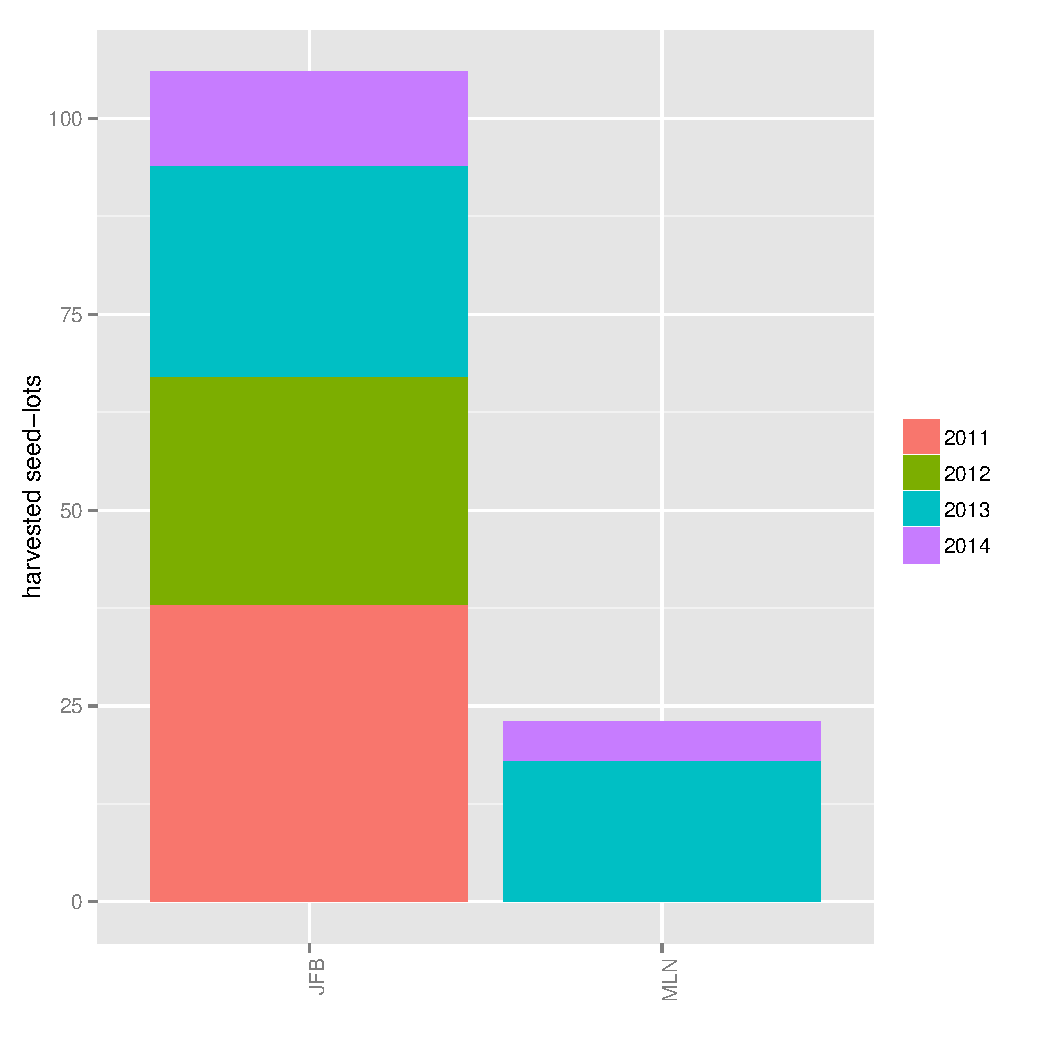
\includegraphics[width=.4\textwidth]{figures/shinemas2R_unnamed-chunk-41-1} 

}



\end{knitrout}
&
\begin{knitrout}
\definecolor{shadecolor}{rgb}{0.969, 0.969, 0.969}\color{fgcolor}

{\centering 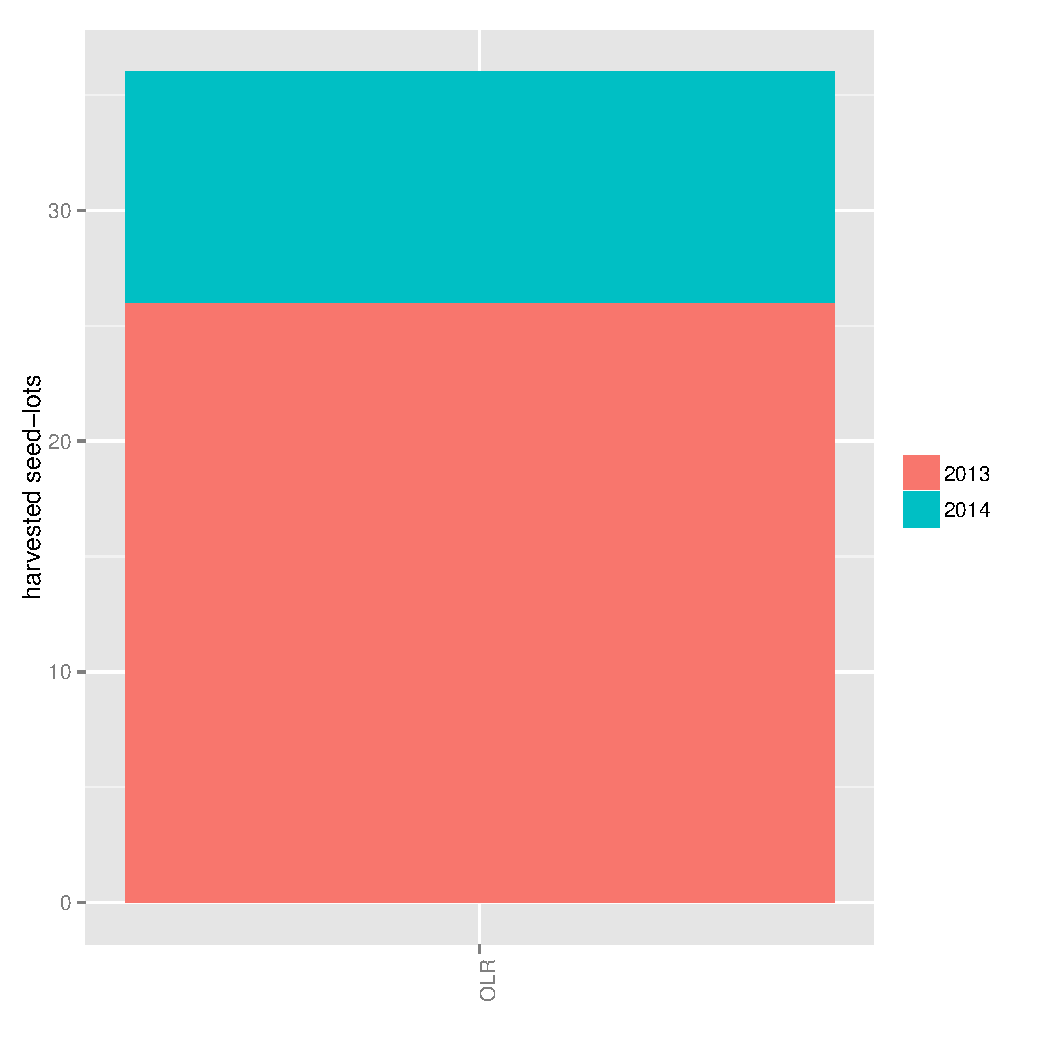
\includegraphics[width=.4\textwidth]{figures/shinemas2R_unnamed-chunk-42-1} 

}



\end{knitrout}
\\
\texttt{p12\_slh\_bw} &  \\
\begin{knitrout}
\definecolor{shadecolor}{rgb}{0.969, 0.969, 0.969}\color{fgcolor}

{\centering 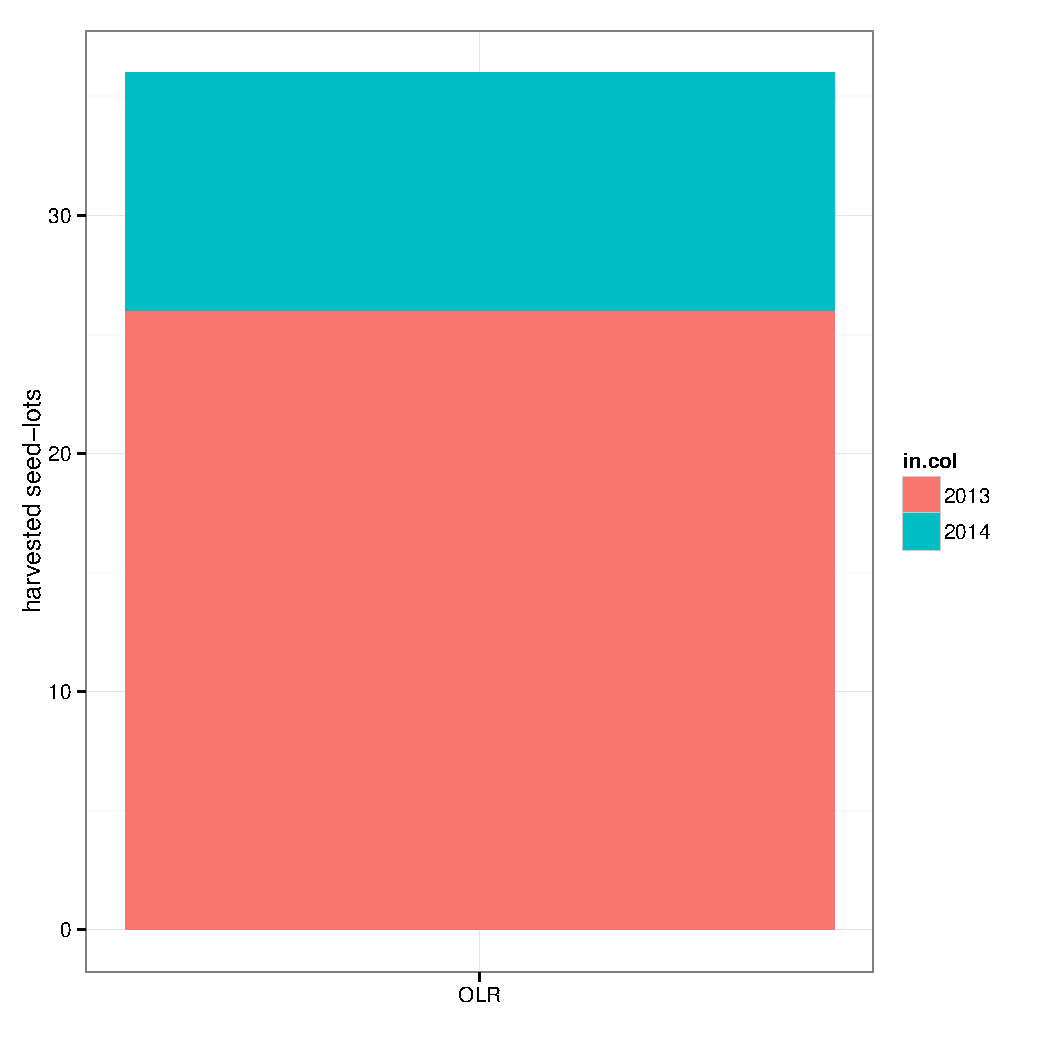
\includegraphics[width=.4\textwidth]{figures/shinemas2R_unnamed-chunk-43-1} 

}



\end{knitrout}
&
\\
\end{tabular}
\end{center}



Or for \texttt{in.col}:
\begin{knitrout}
\definecolor{shadecolor}{rgb}{0.969, 0.969, 0.969}\color{fgcolor}\begin{kframe}
\begin{alltt}
\hlstd{p2_slh} \hlkwb{=} \hlkwd{get.ggplot}\hlstd{(}
        \hlstd{data_network,}
        \hlkwc{ggplot.type} \hlstd{=} \hlstr{"network-reproduction-harvested"}\hlstd{,}
        \hlkwc{ggplot.display} \hlstd{=} \hlstr{"barplot"}\hlstd{,}
        \hlkwc{x.axis} \hlstd{=} \hlstr{"person"}\hlstd{,}
        \hlkwc{in.col} \hlstd{=} \hlstr{"year"}\hlstd{,}
        \hlkwc{nb_parameters_per_plot_in.col} \hlstd{=} \hlnum{2}
        \hlstd{)}

\hlstd{p21_slh} \hlkwb{=} \hlstd{p2_slh}\hlopt{$}\hlstd{`network-reproduction-harvested`}\hlopt{$}\hlstd{barplot}\hlopt{$}\hlstd{`person-year`}\hlopt{$}\hlstd{`x.axis-1|in.col-1`}
\hlstd{p22_slh} \hlkwb{=} \hlstd{p2_slh}\hlopt{$}\hlstd{`network-reproduction-harvested`}\hlopt{$}\hlstd{barplot}\hlopt{$}\hlstd{`person-year`}\hlopt{$}\hlstd{`x.axis-1|in.col-2`}
\end{alltt}
\end{kframe}
\end{knitrout}

\begin{center}
\begin{tabular}{cc}
\texttt{p21\_slh} & \texttt{p22\_slh} \\
\begin{knitrout}
\definecolor{shadecolor}{rgb}{0.969, 0.969, 0.969}\color{fgcolor}

{\centering 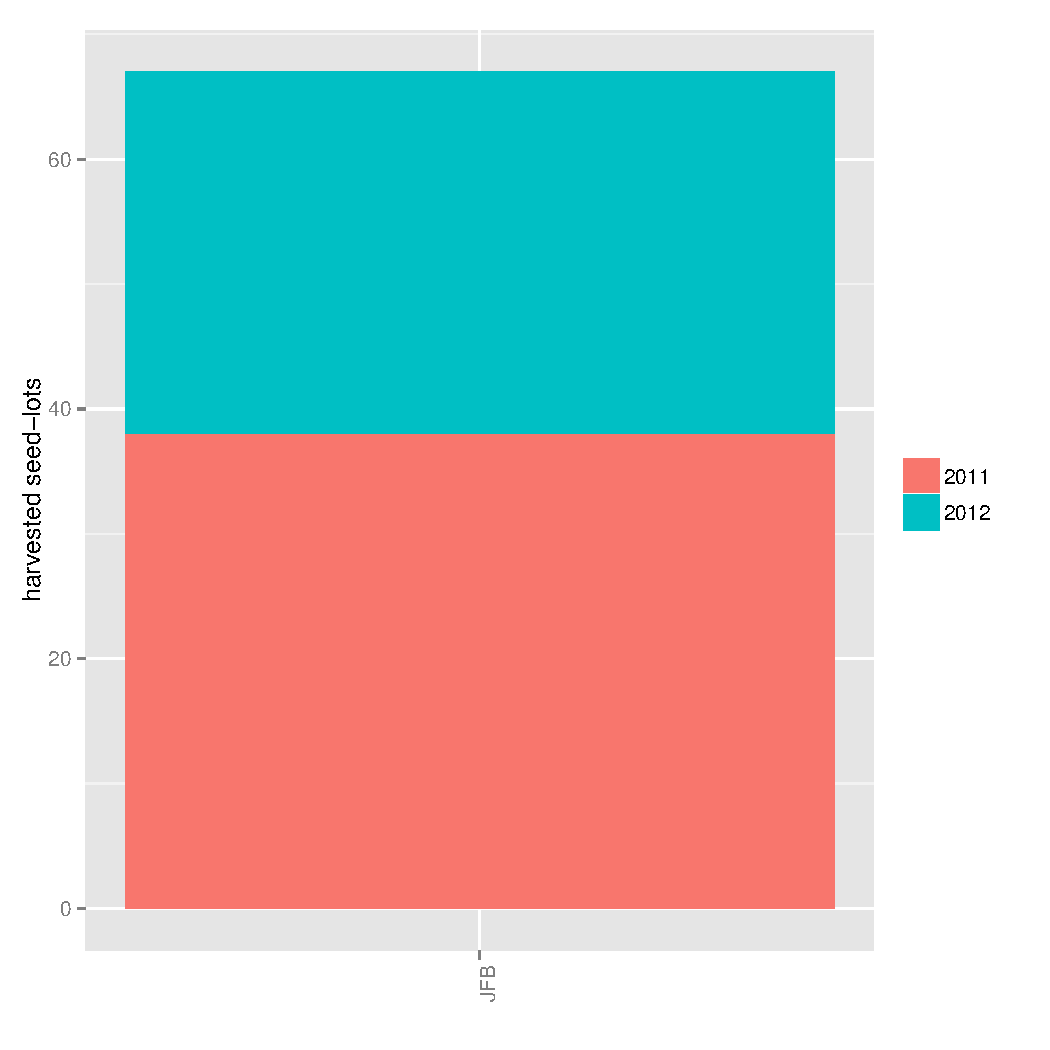
\includegraphics[width=.4\textwidth]{figures/shinemas2R_unnamed-chunk-45-1} 

}



\end{knitrout}
&
\begin{knitrout}
\definecolor{shadecolor}{rgb}{0.969, 0.969, 0.969}\color{fgcolor}

{\centering 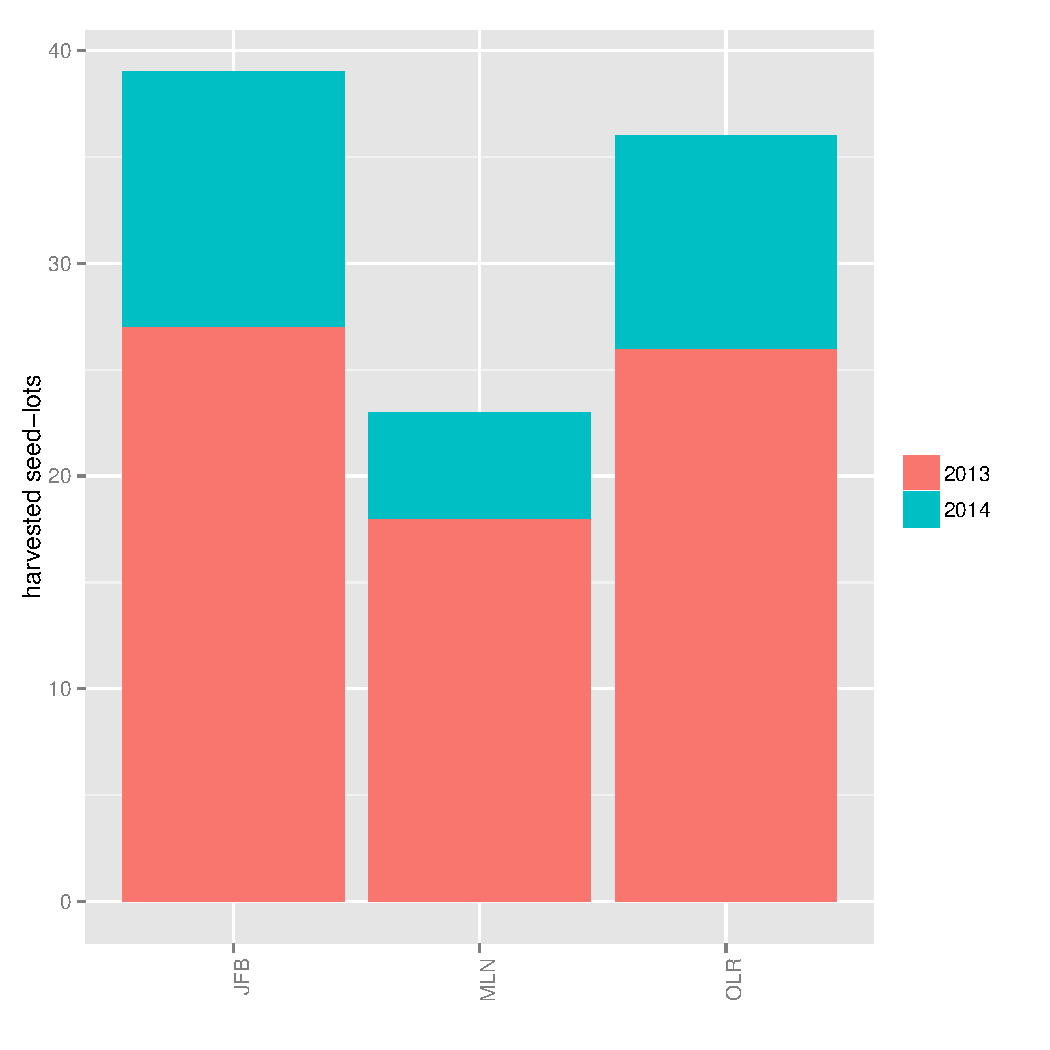
\includegraphics[width=.4\textwidth]{figures/shinemas2R_unnamed-chunk-46-1} 

}



\end{knitrout}
\\
\end{tabular}
\end{center}


Or for both, for each subset of \texttt{x.axis}, you have the set of \texttt{in.col}.

\end{itemize}


\paragraph{\texttt{ggplot.display = map}}

There are as many maps as years and a map with all the years mixed.
The scale represent the number of seed-lots harvested.

\begin{itemize}

\item Default arguments

\begin{knitrout}
\definecolor{shadecolor}{rgb}{0.969, 0.969, 0.969}\color{fgcolor}\begin{kframe}
\begin{alltt}
\hlstd{m_slh} \hlkwb{=} \hlstd{default_network_ggplot}\hlopt{$}\hlstd{`network-reproduction-harvested`}\hlopt{$}\hlstd{map}
\hlkwd{names}\hlstd{(m_slh)}
\end{alltt}
\begin{verbatim}
## [1] "map-[2011]"                   "map-[2012]"                  
## [3] "map-[2013]"                   "map-[2014]"                  
## [5] "map-[2011, 2012, 2013, 2014]"
\end{verbatim}
\begin{alltt}
\hlstd{m1_slh} \hlkwb{=} \hlstd{m_slh}\hlopt{$}\hlstd{`map-[2011]`}
\hlstd{m5_slh} \hlkwb{=} \hlstd{m_slh}\hlopt{$}\hlstd{`map-[2011, 2012, 2013, 2014]`}
\end{alltt}
\end{kframe}
\end{knitrout}

\begin{center}
\begin{tabular}{cc}
\texttt{m1\_slh} & \texttt{m5\_slh} \\
\begin{knitrout}
\definecolor{shadecolor}{rgb}{0.969, 0.969, 0.969}\color{fgcolor}

{\centering 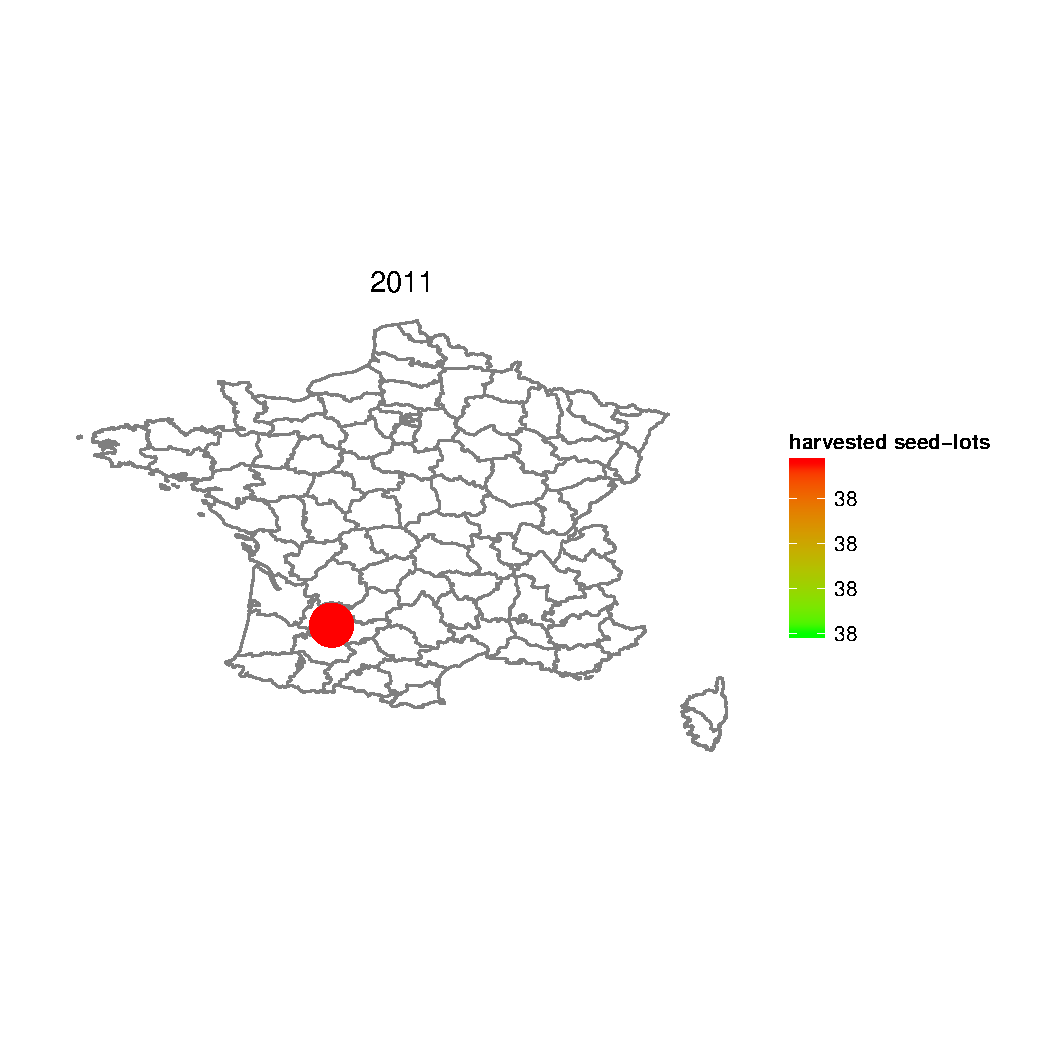
\includegraphics[width=.4\textwidth]{figures/shinemas2R_unnamed-chunk-48-1} 

}



\end{knitrout}
&
\begin{knitrout}
\definecolor{shadecolor}{rgb}{0.969, 0.969, 0.969}\color{fgcolor}

{\centering 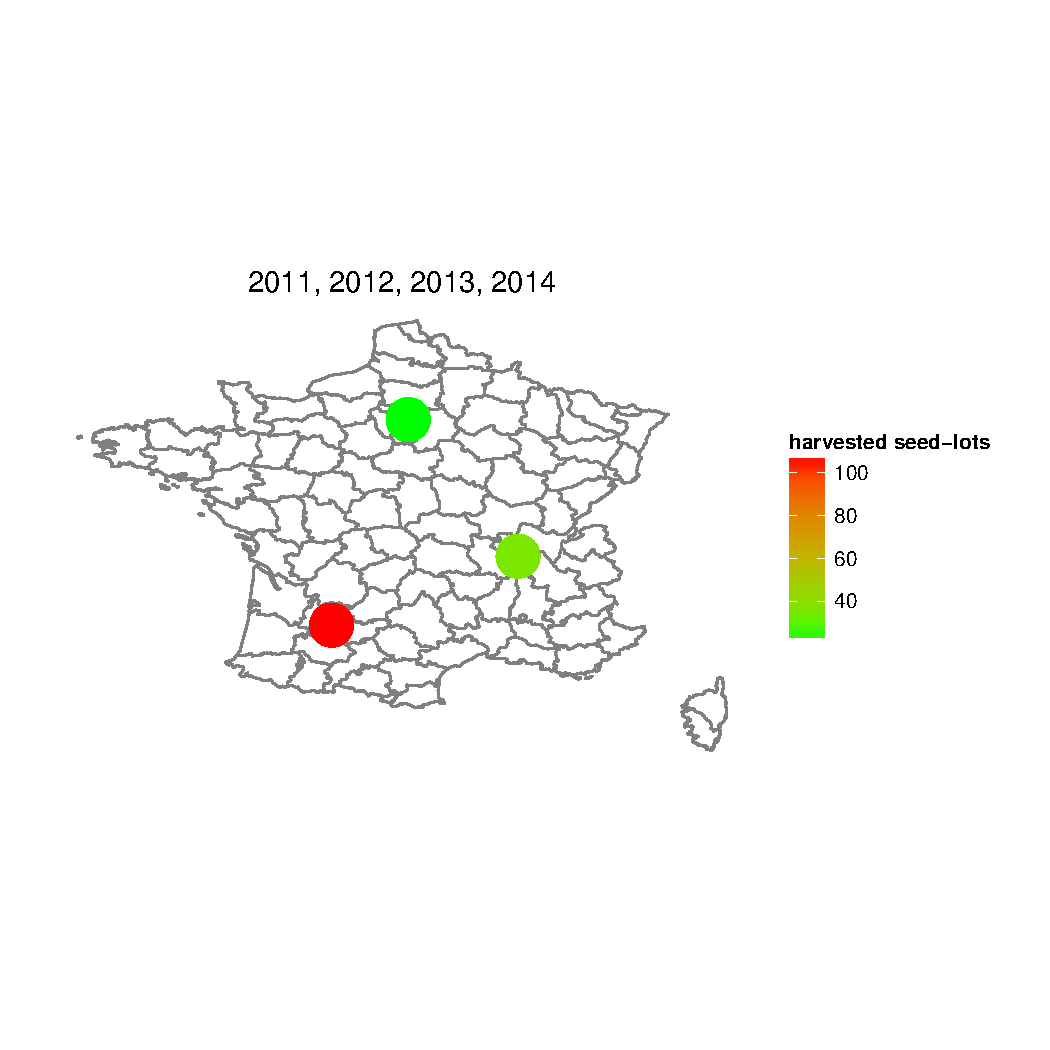
\includegraphics[width=.4\textwidth]{figures/shinemas2R_unnamed-chunk-49-1} 

}



\end{knitrout}
\\
\end{tabular}
\end{center}


\item Custom arguments

It is possible to tune the following arguments (Table \ref{custom.map}):

\begin{center}
\begin{table}[H]
\begin{tabular}{ p{.2\textwidth} p{.15\textwidth} p{.5\textwidth} }
\hline
argument & default value & description \\
\hline

\texttt{hide.labels.parts} & \texttt{NULL} & can be NULL or "all" as only person can be display. \texttt{NULL} by default \\
\hline

\texttt{labels.size} & \texttt{3} & size of the labels \\
\hline

\texttt{location.map} & \texttt{"france"} & location of the map see \texttt{?map} for more details \\
\hline

\texttt{pie.size} & \texttt{.5} & size of the pie when using pies \\

\hline
\end{tabular}
\caption{Possible arguments to custom arguments regarding maps.}
\label{custom.map}
\end{table}
\end{center}

For example,

\begin{knitrout}
\definecolor{shadecolor}{rgb}{0.969, 0.969, 0.969}\color{fgcolor}\begin{kframe}
\begin{alltt}
\hlstd{p_slh} \hlkwb{=} \hlkwd{get.ggplot}\hlstd{(}
        \hlstd{data_network,}
        \hlkwc{ggplot.type} \hlstd{=} \hlstr{"network-reproduction-harvested"}\hlstd{,}
        \hlkwc{ggplot.display} \hlstd{=} \hlstr{"map"}\hlstd{,}
        \hlkwc{hide.labels.parts} \hlstd{=} \hlkwa{NULL}
        \hlstd{)}

\hlstd{p_slh}\hlopt{$}\hlstd{`network-reproduction-harvested`}\hlopt{$}\hlstd{map}\hlopt{$}\hlstd{`map-[2014]`}
\end{alltt}
\end{kframe}

{\centering 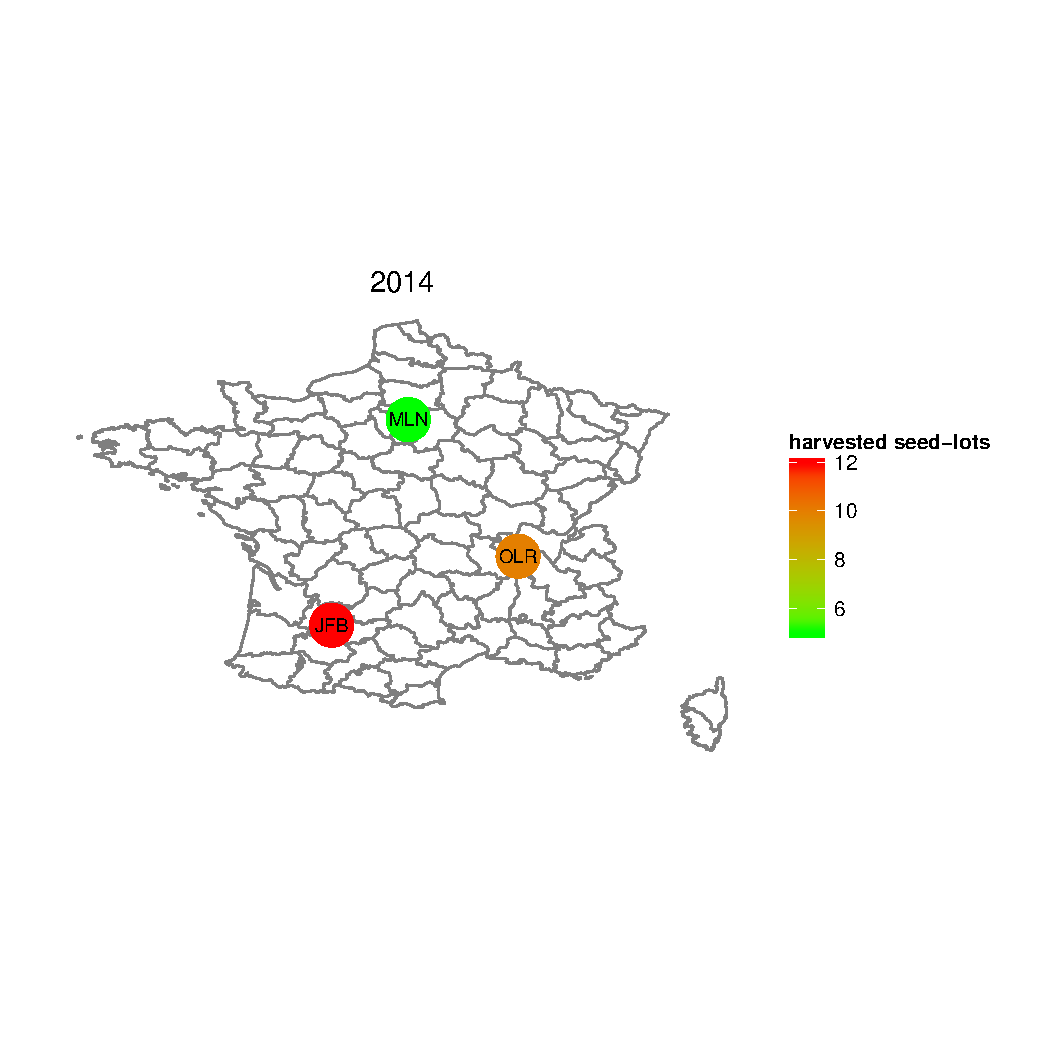
\includegraphics[width=.6\textwidth]{figures/shinemas2R_unnamed-chunk-50-1} 

}



\end{knitrout}

\end{itemize}

\subsubsection{\texttt{ggplot.type = "network-diffusion-relation"}}

\texttt{ggplot.type = "network-diffusion-relation"} corresponds to diffusion of seed-lots on a map.
Note that \texttt{ggplot.display} is useless here.

There are as many maps as years and a map with all the years mixed.
The size of the arrows is proprotionnal to the number of diffusions (\texttt{nb\_diffusions}).

\begin{itemize}

\item Default arguments

\begin{knitrout}
\definecolor{shadecolor}{rgb}{0.969, 0.969, 0.969}\color{fgcolor}\begin{kframe}
\begin{alltt}
\hlstd{m_dr} \hlkwb{=} \hlstd{default_network_ggplot}\hlopt{$}\hlstd{`network-diffusion-relation`}\hlopt{$}\hlstd{map}
\hlkwd{names}\hlstd{(m_dr)}
\end{alltt}
\begin{verbatim}
## [1] "map-[2012]"       "map-[2014]"       "map-[2012, 2014]"
\end{verbatim}
\begin{alltt}
\hlstd{m1_dr} \hlkwb{=} \hlstd{m_dr}\hlopt{$}\hlstd{`map-[2012]`}
\hlstd{m3_dr} \hlkwb{=} \hlstd{m_dr}\hlopt{$}\hlstd{`map-[2012, 2014]`}
\end{alltt}
\end{kframe}
\end{knitrout}

\begin{center}
\begin{tabular}{cc}
\texttt{m1\_dr} & \texttt{m3\_dr} \\
\begin{knitrout}
\definecolor{shadecolor}{rgb}{0.969, 0.969, 0.969}\color{fgcolor}

{\centering 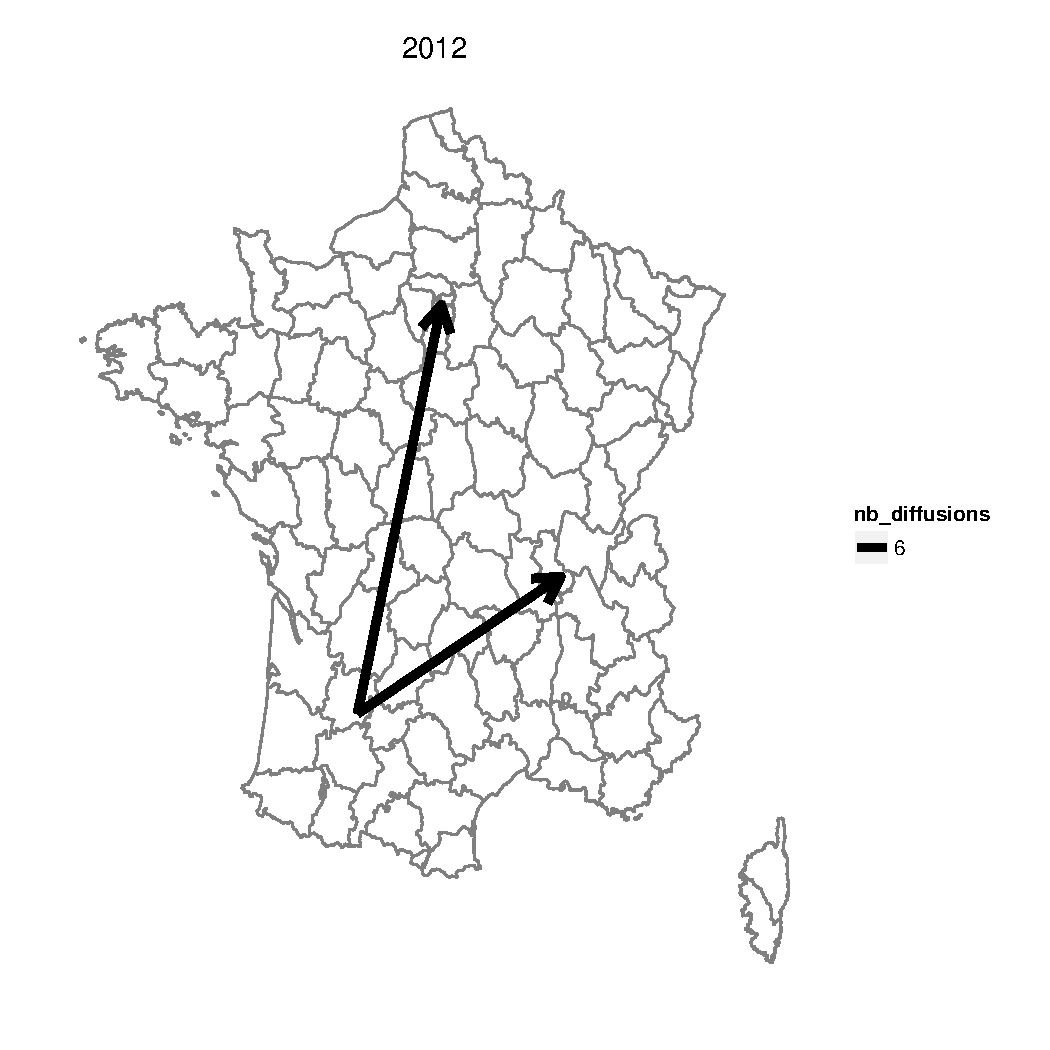
\includegraphics[width=.4\textwidth]{figures/shinemas2R_unnamed-chunk-52-1} 

}



\end{knitrout}
&
\begin{knitrout}
\definecolor{shadecolor}{rgb}{0.969, 0.969, 0.969}\color{fgcolor}

{\centering 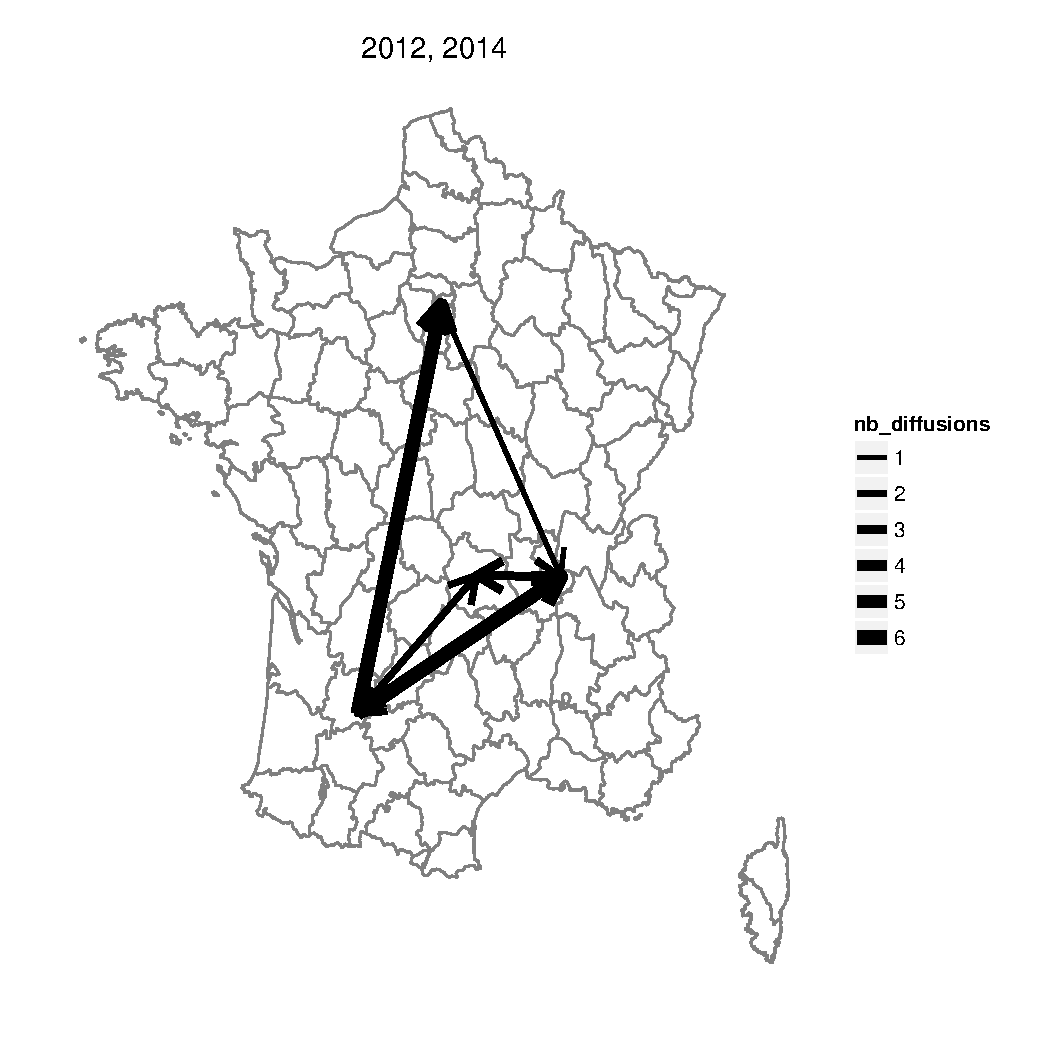
\includegraphics[width=.4\textwidth]{figures/shinemas2R_unnamed-chunk-53-1} 

}



\end{knitrout}
\\
\end{tabular}
\end{center}


\item Custom arguments

Arguments can be customized related to maps. See Table \ref{custom.map}.

\end{itemize}


\subsubsection{\texttt{ggplot.type = "network-reproduction-crossed"}}

Information on the crosses, their parents (mother and father) and grandparents (grandmother and grandfather).
It may be useful to know information on grandparents, especially location, if the cross have been done on another location.

Note that in this example, it represents all the cross where \texttt{Rouge-du-Roc} is involved as \texttt{"father"} or \texttt{"son"} in relation.
This is because in \texttt{get.data}, the following arguments were set: \texttt{germplasm.in = Rouge-du-Roc} and \texttt{filter.on = "father-son"}.


\begin{itemize}

\item Default arguments

\begin{knitrout}
\definecolor{shadecolor}{rgb}{0.969, 0.969, 0.969}\color{fgcolor}\begin{kframe}
\begin{alltt}
\hlstd{cb} \hlkwb{=} \hlstd{default_network_ggplot}\hlopt{$}\hlstd{`network-reproduction-crossed`}\hlopt{$}\hlstd{barplot}
\hlkwd{names}\hlstd{(cb)}
\end{alltt}
\begin{verbatim}
## [1] "cross"       "father"      "grandfather" "mother"     
## [5] "grandmother"
\end{verbatim}
\begin{alltt}
\hlstd{cm} \hlkwb{=} \hlstd{default_network_ggplot}\hlopt{$}\hlstd{`network-reproduction-crossed`}\hlopt{$}\hlstd{map}
\hlkwd{names}\hlstd{(cm)}
\end{alltt}
\begin{verbatim}
## [1] "cross"       "father"      "grandfather" "mother"     
## [5] "grandmother"
\end{verbatim}
\end{kframe}
\end{knitrout}

For example:

\begin{knitrout}
\definecolor{shadecolor}{rgb}{0.969, 0.969, 0.969}\color{fgcolor}\begin{kframe}
\begin{alltt}
\hlstd{cb}\hlopt{$}\hlstd{cross}\hlopt{$}\hlstd{barplot}\hlopt{$}\hlstd{`year-germplasm`}\hlopt{$}\hlstd{`x.axis-1|in.col-1`}
\end{alltt}
\end{kframe}

{\centering 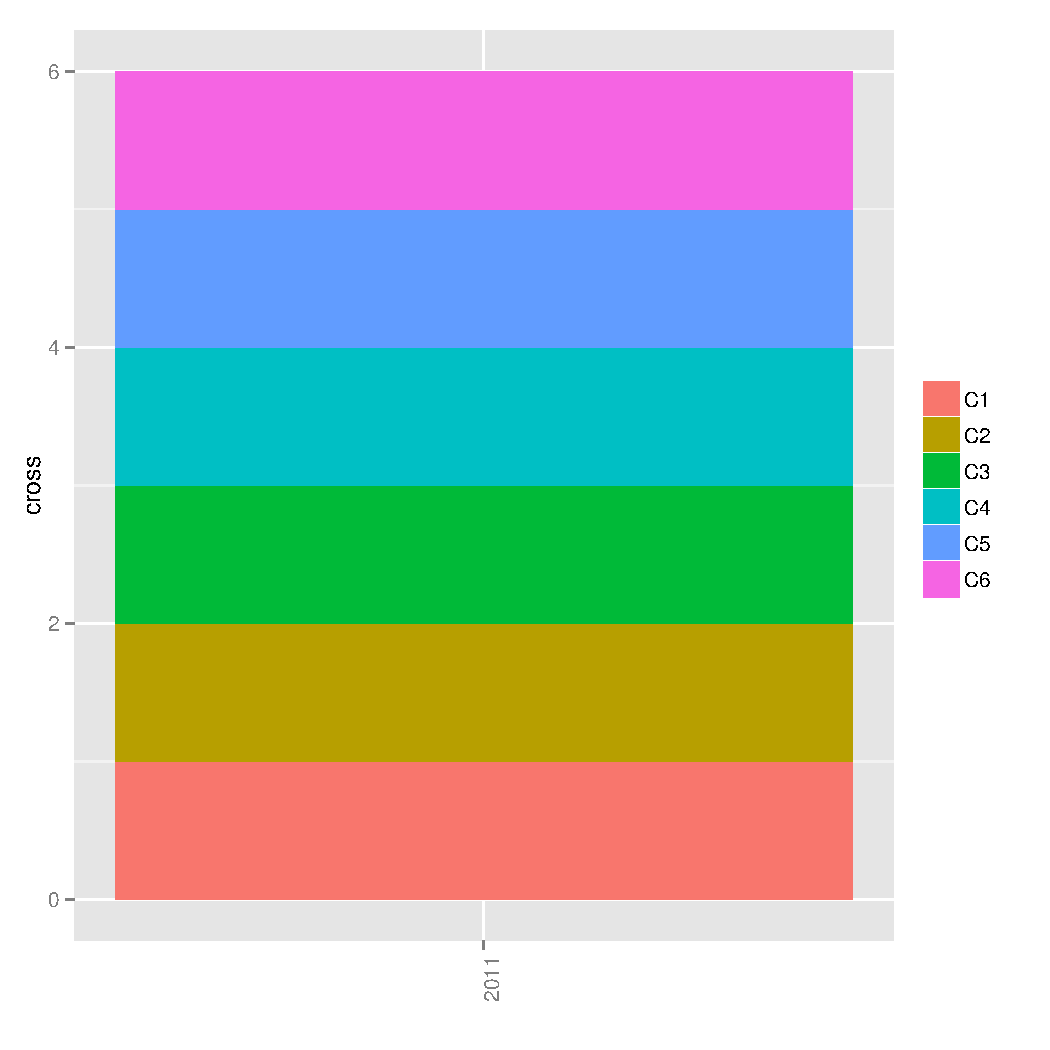
\includegraphics[width=.6\textwidth]{figures/shinemas2R_unnamed-chunk-55-1} 

}



\end{knitrout}

\begin{knitrout}
\definecolor{shadecolor}{rgb}{0.969, 0.969, 0.969}\color{fgcolor}\begin{kframe}
\begin{alltt}
\hlstd{cm}\hlopt{$}\hlstd{cross}\hlopt{$}\hlstd{map}\hlopt{$}\hlstd{`map-[2011]`}
\end{alltt}
\end{kframe}

{\centering 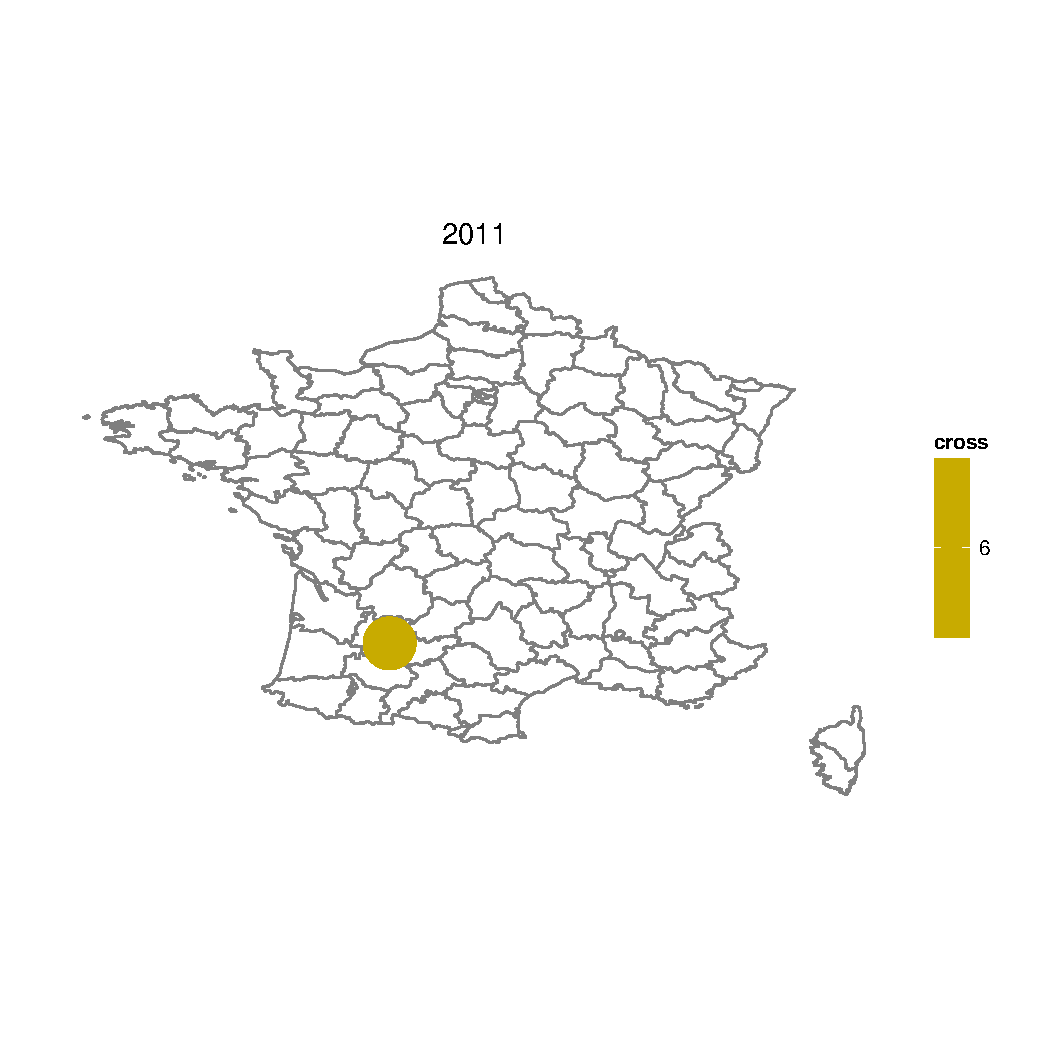
\includegraphics[width=.6\textwidth]{figures/shinemas2R_unnamed-chunk-56-1} 

}



\end{knitrout}

\item Custom arguments

Arguments can be customed related to barplots (Table \ref{custom.barplot}) or maps (Table \ref{custom.map}).

\end{itemize}

\subsubsection{Others \texttt{ggplot.type}}

For the other \texttt{ggplot.type}, as it is exactly the same type of plots than for
\texttt{ggplot.type = "network-reproduction-harvested"}, no example is displayed in this vignette.

The following table describe the different \texttt{ggplot.type}:

\begin{center}
\begin{tabular}{ p{.5\textwidth} p{.5\textwidth} }
\hline
\texttt{ggplot.type} & description \\
\hline

\texttt{"network-reproduction-sown"} & seed-lots that have been sown. \\

\texttt{"network-reproduction-positive-inter-selected"} & seed-lots that have been harvested after a reproduction and have been sown the next season.
It corresponds to positive inter selection. \\

\texttt{"network-reproduction-negative-inter-selected"} & seed-lots that have been harvested after a reproduction and have NOT been sown the next season.
It corresponds to negative inter selection. \\

\texttt{"network-diffusion-sent"} & seed-lots that have been sent to another location. \\

\texttt{"network-diffusion-received"} & seed-lots that have been received in a given location. \\

\texttt{"network-mixture-real"} & seed-lots that have been 'really' mixed into a mixture. \\

\texttt{"network-mixture-rep"} & seed-lots coming from replication that have been mixed into a mixture. Note that it is \texttt{NULL} when the argument \texttt{mixrep\_to\_repro} in \texttt{get.data} is \texttt{TRUE} (default argument).\\

\texttt{"network-mixture-all"} & seed-lots that have been mixed into a mixture (i.e. \texttt{"network-mixture-real"} + \texttt{"network-mixture-rep"}. \\

\texttt{"network-positive-intra-selected"} & seed-lots where intra germplasm selection have been done.
It corresponds to mass selection. \\

\hline
\end{tabular}
\end{center}


\subsection{Get the tables}

It is possible to get the table from the data used for the plot.
For example,

\begin{knitrout}
\definecolor{shadecolor}{rgb}{0.969, 0.969, 0.969}\color{fgcolor}\begin{kframe}
\begin{alltt}
\hlstd{p} \hlkwb{=} \hlstd{default_network_ggplot}\hlopt{$}\hlstd{`network-reproduction-crossed`}\hlopt{$}\hlstd{barplot}\hlopt{$}\hlstd{cross}\hlopt{$}\hlstd{barplot}
\hlstd{p} \hlkwb{=} \hlstd{p}\hlopt{$}\hlstd{`year-germplasm`}\hlopt{$}\hlstd{`x.axis-1|in.col-1`}
\hlstd{tab_p} \hlkwb{=} \hlkwd{get.table}\hlstd{(p)}
\hlstd{tab_p}
\end{alltt}
\begin{verbatim}
##   mean germplasm year
## 1    1        C1 2011
## 2    1        C2 2011
## 3    1        C3 2011
## 4    1        C4 2011
## 5    1        C5 2011
## 6    1        C6 2011
\end{verbatim}
\end{kframe}
\end{knitrout}



\newpage


% version 0.9.2
\section{Data linked to the \sl~and to the relations between \sl}
\label{data}


\subsection{Get the data set}

Three types of queries are possible:
\begin{itemize}
\item \texttt{query.type = "data-classic"} to study classic variables for each seed-lot or relation between seed-lots (subsection \ref{data-classic})
\item \texttt{query.type = "data-S"} to study selection differential (subsection \ref{data-S-and-SR})
\item \texttt{query.type = "data-SR"} to study response to selection (subsection \ref{data-S-and-SR})
\end{itemize}

You can set filters to the query with the following argument :

\begin{itemize}
\item \texttt{filter.in} to choose nothing except \texttt{filter.in}
\item \texttt{filter.out} to choose everything except \texttt{filter.out}
\end{itemize}

values of filters can be \texttt{germplasm}, \texttt{germplasm.type}, \texttt{year}, \texttt{person}, \texttt{project}, \texttt{\sl}, \texttt{relation}, \texttt{reproduction.type} or \texttt{variable}.


It is important to choose if you apply the filter on the \texttt{father} or the \texttt{son} of a relation.
This can be done with the argument \texttt{filter.on}.
Possible values are \texttt{"father"}, \texttt{"son"} or \texttt{"father-son"}.


You can either query information on relation between \sl~or on \sl.
This is set with the argument \texttt{data.type}.
Possibles values are 

\begin{itemize}
\item \texttt{"relation"} for data linked to relation between seed lots and 
\item \texttt{"seed-lots"} for data linked to seed lots
\end{itemize}


The function returns a list with
\begin{itemize}
\item a data frame with the data set
\item a list with data set with individuals that are correlated for a set of variables
\item the description of methods used for each variable with its description and units
\end{itemize}

Note that for data linked to seed-lots, all the data are correlated as there is one measure for a given seed-lot. 
Therefore the element of the list for correlated data is always NULL.
For data linked to relations, as it can be linked to individual within a seed-lot, data may be correlated (data taken on ther same individual) or not.

A data set with only correlated variables for each individual is useful when doing multivariate analysis such as PCA.

The names of the variables in the output of the function are under the form \texttt{variable\_name---methods}.

\vspace{.5cm}

In the following examples, three variables are studied:

\begin{knitrout}
\definecolor{shadecolor}{rgb}{0.969, 0.969, 0.969}\color{fgcolor}\begin{kframe}
\begin{alltt}
\hlstd{vec_variables} \hlkwb{=} \hlkwd{c}\hlstd{(}\hlstr{"hauteur"}\hlstd{,} \hlstr{"pmg"}\hlstd{,} \hlstr{"poids_epis"}\hlstd{)}
\end{alltt}
\end{kframe}
\end{knitrout}

\subsubsection{\texttt{query.type = "data-classic"}}
\label{data-classic}
\begin{knitrout}
\definecolor{shadecolor}{rgb}{0.969, 0.969, 0.969}\color{fgcolor}\begin{kframe}
\begin{alltt}
\hlkwa{if}\hlstd{(use.get.data)\{}
        \hlstd{data_classic} \hlkwb{=} \hlkwd{get.data}\hlstd{(}
                \hlkwc{db_user} \hlstd{= info_db}\hlopt{$}\hlstd{db_user,} \hlkwc{db_host} \hlstd{= info_db}\hlopt{$}\hlstd{db_host,} \hlcom{# db infos}
                \hlkwc{db_name} \hlstd{= info_db}\hlopt{$}\hlstd{db_name,} \hlkwc{db_password} \hlstd{= info_db}\hlopt{$}\hlstd{db_password,} \hlcom{# db infos}
                \hlkwc{query.type} \hlstd{=} \hlstr{"data-classic"}\hlstd{,} \hlcom{# data-classic query}
                \hlkwc{person.in} \hlstd{=} \hlstr{"JFB"}\hlstd{,} \hlcom{# person to keep}
                \hlkwc{filter.on} \hlstd{=} \hlstr{"father-son"}\hlstd{,} \hlcom{# filters on father AND son}
                \hlkwc{data.type} \hlstd{=} \hlstr{"relation"}\hlstd{,} \hlcom{# data linked to relation between seed-lots}
                \hlkwc{variable} \hlstd{= vec_variables,} \hlcom{# the variables to display}
                \hlkwc{project.in} \hlstd{=} \hlstr{"DEMO"} \hlcom{# the project }
                \hlstd{)}
\hlstd{\}} \hlkwa{else} \hlstd{\{}
        \hlcom{# 1. Query SHiNeMaS ...}
        \hlcom{# 2. Set up data set ...}
        \hlcom{# |==========================================================| 100%}

        \hlkwd{load}\hlstd{(}\hlstr{"./data/data_classic.RData"}\hlstd{)}
\hlstd{\}}

\hlkwd{names}\hlstd{(data_classic}\hlopt{$}\hlstd{data)}
\end{alltt}
\begin{verbatim}
## [1] "data"                          
## [2] "data.with.correlated.variables"
## [3] "methods"
\end{verbatim}
\begin{alltt}
\hlkwd{colnames}\hlstd{(data_classic}\hlopt{$}\hlstd{data}\hlopt{$}\hlstd{data)}
\end{alltt}
\begin{verbatim}
##  [1] "son_species"                  "son_project"                 
##  [3] "son"                          "son_ind"                     
##  [5] "son_year"                     "son_germplasm"               
##  [7] "son_germplasm_type"           "son_person"                  
##  [9] "son_alt"                      "son_long"                    
## [11] "son_lat"                      "son_total_generation_nb"     
## [13] "son_local_generation_nb"      "son_generation_confidence"   
## [15] "son_comments"                 "father_species"              
## [17] "father_project"               "father"                      
## [19] "father_year"                  "father_germplasm"            
## [21] "father_germplasm_type"        "father_person"               
## [23] "father_alt"                   "father_long"                 
## [25] "father_lat"                   "father_total_generation_nb"  
## [27] "father_local_generation_nb"   "father_generation_confidence"
## [29] "father_comments"              "reproduction_id"             
## [31] "reproduction_method_name"     "selection_id"                
## [33] "selection_person"             "mixture_id"                  
## [35] "diffusion_id"                 "relation_year_start"         
## [37] "relation_year_end"            "X"                           
## [39] "Y"                            "block"                       
## [41] "hauteur---hauteur_tige"       "hauteur---hauteur_tige$date" 
## [43] "pmg---pmg"                    "pmg---pmg-2"                 
## [45] "pmg---pmg-2$date"             "pmg---pmg$date"              
## [47] "poids_epis---poids_epis"      "poids_epis---poids_epis$date"
\end{verbatim}
\begin{alltt}
\hlkwd{head}\hlstd{(data_classic}\hlopt{$}\hlstd{data}\hlopt{$}\hlstd{methods)}
\end{alltt}
\begin{verbatim}
##    method_name variable_name method_description unit
## 1 hauteur_tige       hauteur                        
## 2   poids_epis    poids_epis                        
## 3          pmg           pmg                        
## 4        pmg-2           pmg                        
##        variable---methods
## 1  hauteur---hauteur_tige
## 2 poids_epis---poids_epis
## 3               pmg---pmg
## 4             pmg---pmg-2
\end{verbatim}
\end{kframe}
\end{knitrout}

The data with correlated variables :

\begin{knitrout}
\definecolor{shadecolor}{rgb}{0.969, 0.969, 0.969}\color{fgcolor}\begin{kframe}
\begin{alltt}
\hlkwd{names}\hlstd{(data_classic}\hlopt{$}\hlstd{data}\hlopt{$}\hlstd{data.with.correlated.variables)}
\end{alltt}
\begin{verbatim}
## [1] "A_2013" "B_2013" "A_2014" "B_2014"
\end{verbatim}
\end{kframe}
\end{knitrout}

The methods related to each variable :

\begin{knitrout}
\definecolor{shadecolor}{rgb}{0.969, 0.969, 0.969}\color{fgcolor}\begin{kframe}
\begin{alltt}
\hlstd{data_classic}\hlopt{$}\hlstd{data}\hlopt{$}\hlstd{methods}
\end{alltt}
\begin{verbatim}
##    method_name variable_name method_description unit
## 1 hauteur_tige       hauteur                        
## 2   poids_epis    poids_epis                        
## 3          pmg           pmg                        
## 4        pmg-2           pmg                        
##        variable---methods
## 1  hauteur---hauteur_tige
## 2 poids_epis---poids_epis
## 3               pmg---pmg
## 4             pmg---pmg-2
\end{verbatim}
\end{kframe}
\end{knitrout}

\subsubsection{Selection differential (\texttt{query.type = "data-S"}), response to selection (\texttt{query.type = "data-SR"}) and heritability}
\label{data-S-and-SR}

For a given trait, selection differential corresponds to the difference between mean of the selected spikes and mean of the bulk (i.e. spikes that have not been selected).
Response to selection correponds to the difference between mean of spikes coming from the selected spikes and the spikes coming from the bulk (Figure \ref{SandR}).

Selection differential ($S$) and response to selection ($R$) are linked with the realized heritability ($h_{r}^2$):

\begin{displaymath}
R = h_{r}^2 \times S
\end{displaymath}

See appendix \ref{text_SandR} for more details on the theory behind this.

\begin{figure}[H]
\begin{center}
\includegraphics[page=8, width=.8\textwidth]{SandR_EN.pdf}
\caption{Seletion differential ($S$) in 2014-2015 and response to selection ($R$) in 2015-2016. Circles and arrows in gray represent the seed-lots that have been sown in 2015 after harvest in 2015.}
\label{SandR}
\end{center}
\end{figure}



\paragraph{\texttt{query.type = "data-S"}}

The data frame returned has a column \texttt{"expe"} which corresponds to an id of one selection differential.

\begin{knitrout}
\definecolor{shadecolor}{rgb}{0.969, 0.969, 0.969}\color{fgcolor}\begin{kframe}
\begin{alltt}
\hlkwa{if}\hlstd{(use.get.data)\{}
        \hlstd{data_S} \hlkwb{=} \hlkwd{get.data}\hlstd{(}
                \hlkwc{db_user} \hlstd{= info_db}\hlopt{$}\hlstd{db_user,} \hlkwc{db_host} \hlstd{= info_db}\hlopt{$}\hlstd{db_host,}
                \hlkwc{db_name} \hlstd{= info_db}\hlopt{$}\hlstd{db_name,} \hlkwc{db_password} \hlstd{= info_db}\hlopt{$}\hlstd{db_password,}
                \hlkwc{query.type} \hlstd{=} \hlstr{"data-S"}\hlstd{,}
                \hlkwc{person.in} \hlstd{=} \hlstr{"JFB"}\hlstd{,}
                \hlkwc{filter.on} \hlstd{=} \hlstr{"father-son"}\hlstd{,}
                \hlkwc{data.type} \hlstd{=} \hlstr{"relation"}\hlstd{,}
                \hlkwc{variable} \hlstd{= vec_variables,}
                \hlkwc{project.in} \hlstd{=} \hlstr{"DEMO"}
                \hlstd{)}
\hlstd{\}} \hlkwa{else} \hlstd{\{}
        \hlcom{# 1. Query SHiNeMaS ...}
        \hlcom{# 2. Set up data set ...}
        \hlcom{# |==========================================================| 100%}

        \hlkwd{load}\hlstd{(}\hlstr{"./data/data_S.RData"}\hlstd{)}
\hlstd{\}}

\hlkwd{colnames}\hlstd{(data_S}\hlopt{$}\hlstd{data}\hlopt{$}\hlstd{data)}
\end{alltt}
\begin{verbatim}
##  [1] "son"                          "expe"                        
##  [3] "sl_statut"                    "expe_name"                   
##  [5] "expe_name_2"                  "son_species"                 
##  [7] "son_project"                  "son_ind"                     
##  [9] "son_year"                     "son_germplasm"               
## [11] "son_germplasm_type"           "son_person"                  
## [13] "son_alt"                      "son_long"                    
## [15] "son_lat"                      "son_total_generation_nb"     
## [17] "son_local_generation_nb"      "son_generation_confidence"   
## [19] "son_comments"                 "father_species"              
## [21] "father_project"               "father"                      
## [23] "father_year"                  "father_germplasm"            
## [25] "father_germplasm_type"        "father_person"               
## [27] "father_alt"                   "father_long"                 
## [29] "father_lat"                   "father_total_generation_nb"  
## [31] "father_local_generation_nb"   "father_generation_confidence"
## [33] "father_comments"              "reproduction_id"             
## [35] "reproduction_method_name"     "selection_id"                
## [37] "selection_person"             "mixture_id"                  
## [39] "diffusion_id"                 "relation_year_start"         
## [41] "relation_year_end"            "X"                           
## [43] "Y"                            "block"                       
## [45] "hauteur---hauteur_tige"       "hauteur---hauteur_tige$date" 
## [47] "pmg---pmg"                    "pmg---pmg-2"                 
## [49] "pmg---pmg-2$date"             "pmg---pmg$date"              
## [51] "poids_epis---poids_epis"      "poids_epis---poids_epis$date"
\end{verbatim}
\end{kframe}
\end{knitrout}



\paragraph{\texttt{query.type = "data-SR"}}

The data frame returned has a column \texttt{"expe"} which corresponds to an id of one selection differential and the corresponding response to selection

The query takes into account when selection have been done in a seed lot, that this seed lot have been merged and then have been sown. 
It is the case when selection have been carried out in a replication that have been merge afterwards. 
Even if this case should not arise, it might happen.

\begin{knitrout}
\definecolor{shadecolor}{rgb}{0.969, 0.969, 0.969}\color{fgcolor}\begin{kframe}
\begin{alltt}
\hlkwa{if}\hlstd{(use.get.data)\{}
        \hlstd{data_SR} \hlkwb{=} \hlkwd{get.data}\hlstd{(}
                \hlkwc{db_user} \hlstd{= info_db}\hlopt{$}\hlstd{db_user,} \hlkwc{db_host} \hlstd{= info_db}\hlopt{$}\hlstd{db_host,}
                \hlkwc{db_name} \hlstd{= info_db}\hlopt{$}\hlstd{db_name,} \hlkwc{db_password} \hlstd{= info_db}\hlopt{$}\hlstd{db_password,}
                \hlkwc{query.type} \hlstd{=} \hlstr{"data-SR"}\hlstd{,}
                \hlkwc{person.in} \hlstd{=} \hlstr{"JFB"}\hlstd{,}
                \hlkwc{filter.on} \hlstd{=} \hlstr{"father-son"}\hlstd{,}
                \hlkwc{data.type} \hlstd{=} \hlstr{"relation"}\hlstd{,}
                \hlkwc{variable} \hlstd{= vec_variables,}
                \hlkwc{project.in} \hlstd{=} \hlstr{"DEMO"}
                \hlstd{)}
\hlstd{\}} \hlkwa{else} \hlstd{\{}
        \hlcom{# 1. Query SHiNeMaS ...}
        \hlcom{# 2. Set up data set ...}
        \hlcom{# |==========================================================| 100%}

        \hlkwd{load}\hlstd{(}\hlstr{"./data/data_SR.RData"}\hlstd{)}
\hlstd{\}}

\hlkwd{colnames}\hlstd{(data_SR}\hlopt{$}\hlstd{data}\hlopt{$}\hlstd{data)}
\end{alltt}
\begin{verbatim}
##  [1] "son"                          "expe"                        
##  [3] "sl_statut"                    "expe_name"                   
##  [5] "expe_name_2"                  "son_species"                 
##  [7] "son_project"                  "son_ind"                     
##  [9] "son_year"                     "son_germplasm"               
## [11] "son_germplasm_type"           "son_person"                  
## [13] "son_alt"                      "son_long"                    
## [15] "son_lat"                      "son_total_generation_nb"     
## [17] "son_local_generation_nb"      "son_generation_confidence"   
## [19] "son_comments"                 "father_species"              
## [21] "father_project"               "father"                      
## [23] "father_year"                  "father_germplasm"            
## [25] "father_germplasm_type"        "father_person"               
## [27] "father_alt"                   "father_long"                 
## [29] "father_lat"                   "father_total_generation_nb"  
## [31] "father_local_generation_nb"   "father_generation_confidence"
## [33] "father_comments"              "reproduction_id"             
## [35] "reproduction_method_name"     "selection_id"                
## [37] "selection_person"             "mixture_id"                  
## [39] "diffusion_id"                 "relation_year_start"         
## [41] "relation_year_end"            "X"                           
## [43] "Y"                            "block"                       
## [45] "hauteur---hauteur_tige"       "hauteur---hauteur_tige$date" 
## [47] "pmg---pmg"                    "pmg---pmg-2"                 
## [49] "pmg---pmg-2$date"             "pmg---pmg$date"              
## [51] "poids_epis---poids_epis"      "poids_epis---poids_epis$date"
\end{verbatim}
\end{kframe}
\end{knitrout}


\subsection{Get the ggplots}

To get the plots, use the function \texttt{get.ggplot}.

First of all ,you need to choose

\begin{itemize}
\item on which data set you get the ggplots.
This can be done on \texttt{correlated\_group} having the following argument:
\begin{itemize}
\item \texttt{NULL}, the default argument (\texttt{shinemas2R::get.data()\$data\$data})
\item the name of a given \texttt{correlation\_group} (\texttt{shinemas2R::get.data()\$data\$data.with.correlated.variables})
\end{itemize}

\item if you want to merge germplasm name and selection name with the argument \texttt{merge\_g\_and\_s} which is \texttt{TRUE} by default
\end{itemize}


The names of the variables are under the form \texttt{variable\_name---methods}:
\begin{knitrout}
\definecolor{shadecolor}{rgb}{0.969, 0.969, 0.969}\color{fgcolor}\begin{kframe}
\begin{alltt}
\hlstd{plot_vec_variables} \hlkwb{=} \hlkwd{c}\hlstd{(}
        \hlstr{"hauteur---hauteur_tige"}\hlstd{,}
        \hlstr{"pmg---pmg"}\hlstd{,}
        \hlstr{"poids_epis---poids_epis"}
        \hlstd{)}
\end{alltt}
\end{kframe}
\end{knitrout}

\subsubsection{ggplots for \texttt{data-classic} }

\begin{itemize}

\item barplot, boxplot, interaction, radar and biplot

\begin{itemize}

\item Default arguments
\begin{knitrout}
\definecolor{shadecolor}{rgb}{0.969, 0.969, 0.969}\color{fgcolor}\begin{kframe}
\begin{alltt}
\hlstd{default_data_classic_ggplot} \hlkwb{=} \hlkwd{get.ggplot}\hlstd{(}
        \hlstd{data_classic,}
        \hlkwc{vec_variables} \hlstd{= plot_vec_variables}
        \hlstd{)}
\end{alltt}


{\ttfamily\noindent\itshape\color{messagecolor}{\#\# As ggplot.type is NULL, ggplot.Type is set to data-barplot, data-boxplot, data-interaction, data-radar, data-biplot\\\#\# As x.axis and in.col are NULL, all the combinaisons of x.axis and in.col are done for data-barplot, data-boxplot and data-interaction.\\\#\# As in.col is NULL, each in.col are done for data-radar and data-biplot.}}\begin{verbatim}
## [1] "A Virer quand les données seront propres dans get.data"
## [1] "A Virer quand les données seront propres dans get.data"
## [1] "A Virer quand les données seront propres dans get.data"
\end{verbatim}


{\ttfamily\noindent\itshape\color{messagecolor}{\#\# For data-biplot, hide.labels.parts has been set to NULL instead of "{}all"{}.}}\end{kframe}
\end{knitrout}

By default, the following plots are done:
\begin{knitrout}
\definecolor{shadecolor}{rgb}{0.969, 0.969, 0.969}\color{fgcolor}\begin{kframe}
\begin{alltt}
\hlkwd{names}\hlstd{(default_data_classic_ggplot)}
\end{alltt}
\begin{verbatim}
## [1] "data-barplot"     "data-boxplot"     "data-interaction"
## [4] "data-radar"       "data-biplot"
\end{verbatim}
\end{kframe}
\end{knitrout}

which correpond to \texttt{ggplot.type} arguments:

\begin{center}
\begin{tabular}{ p{.3\textwidth} p{.6\textwidth} }
\hline
\texttt{ggplot.type} & description \\
\hline

\texttt{"data-barplot"} &  barplot, there is one barplot per variable \\

\texttt{"data-boxplot"} &  boxplot, there is one boxplot per variable \\

\texttt{"data-interaction"} &  interaction, there is one interation plot per variable \\

\texttt{"data-radar"} &  radar, there is one radar per set of variables (i.e. the whole \texttt{vec\_variables}). It is the mean that is represented. \\

\texttt{"data-biplot"} &  biplot, there is one biplot per pairs of variables.
Note that no plots are possible for between raw data linked to individuals and raw data linked to relation. \\

\hline
\end{tabular}
\end{center}

For \texttt{ggplot.type = } \texttt{data-barplot}, \texttt{data-boxplot} and \texttt{data-interaction}, you may chose what you want in the x axis (\texttt{x.axis} argument) and in color (\texttt{in.col} argument).
The possible values for \texttt{x.axis} and \texttt{in.col} are: \texttt{germplasm}, \texttt{year}, \texttt{person}.
By default all combinaisons of \texttt{x.axis} and \texttt{in.col} are done with default argument settings.
The name of the plot is under the form \texttt{x.axis}-\texttt{in.col}.

\begin{knitrout}
\definecolor{shadecolor}{rgb}{0.969, 0.969, 0.969}\color{fgcolor}\begin{kframe}
\begin{alltt}
\hlkwd{names}\hlstd{(default_data_classic_ggplot}\hlopt{$}\hlstd{`data-barplot`)}
\end{alltt}
\begin{verbatim}
## [1] "germplasm-year"   "germplasm-person" "person-year"     
## [4] "person-germplasm" "year-person"      "year-germplasm"
\end{verbatim}
\end{kframe}
\end{knitrout}

Knowing a combinaison of \texttt{x.axis} and \texttt{in.col}, choose the variable you want to get.
For example:

\begin{itemize}
\item For barplot:
\begin{knitrout}
\definecolor{shadecolor}{rgb}{0.969, 0.969, 0.969}\color{fgcolor}\begin{kframe}
\begin{alltt}
\hlstd{p_cal_ph_bar_all} \hlkwb{=} \hlstd{default_data_classic_ggplot}\hlopt{$}\hlstd{`data-barplot`}\hlopt{$}\hlstd{`germplasm-year`}
\hlstd{p_cal_ph_bar} \hlkwb{=} \hlstd{p_cal_ph_bar_all}\hlopt{$}\hlstd{`hauteur---hauteur_tige`}\hlopt{$}\hlstd{`x.axis-1|in.col-1`}
\end{alltt}
\end{kframe}
\end{knitrout}

\item For boxplot:
\begin{knitrout}
\definecolor{shadecolor}{rgb}{0.969, 0.969, 0.969}\color{fgcolor}\begin{kframe}
\begin{alltt}
\hlstd{p_cal_ph_box_all} \hlkwb{=} \hlstd{default_data_classic_ggplot}\hlopt{$}\hlstd{`data-boxplot`}\hlopt{$}\hlstd{`germplasm-year`}
\hlstd{p_cal_ph_box} \hlkwb{=} \hlstd{p_cal_ph_box_all}\hlopt{$}\hlstd{`hauteur---hauteur_tige`}\hlopt{$}\hlstd{`x.axis-1|in.col-1`}
\end{alltt}
\end{kframe}
\end{knitrout}

\item For interaction plot:
\begin{knitrout}
\definecolor{shadecolor}{rgb}{0.969, 0.969, 0.969}\color{fgcolor}\begin{kframe}
\begin{alltt}
\hlstd{p_cal_ph_int_all} \hlkwb{=} \hlstd{default_data_classic_ggplot}\hlopt{$}\hlstd{`data-interaction`}\hlopt{$}\hlstd{`year-germplasm`}
\hlstd{p_cal_ph_int} \hlkwb{=} \hlstd{p_cal_ph_int_all}\hlopt{$}\hlstd{`hauteur---hauteur_tige`}\hlopt{$}\hlstd{`x.axis-1|in.col-1`}
\end{alltt}
\end{kframe}
\end{knitrout}
\end{itemize}


\begin{center}
\begin{tabular}{cc}
\texttt{p\_cal\_ph\_bar} & \texttt{p\_cal\_ph\_box} \\
\begin{knitrout}
\definecolor{shadecolor}{rgb}{0.969, 0.969, 0.969}\color{fgcolor}

{\centering 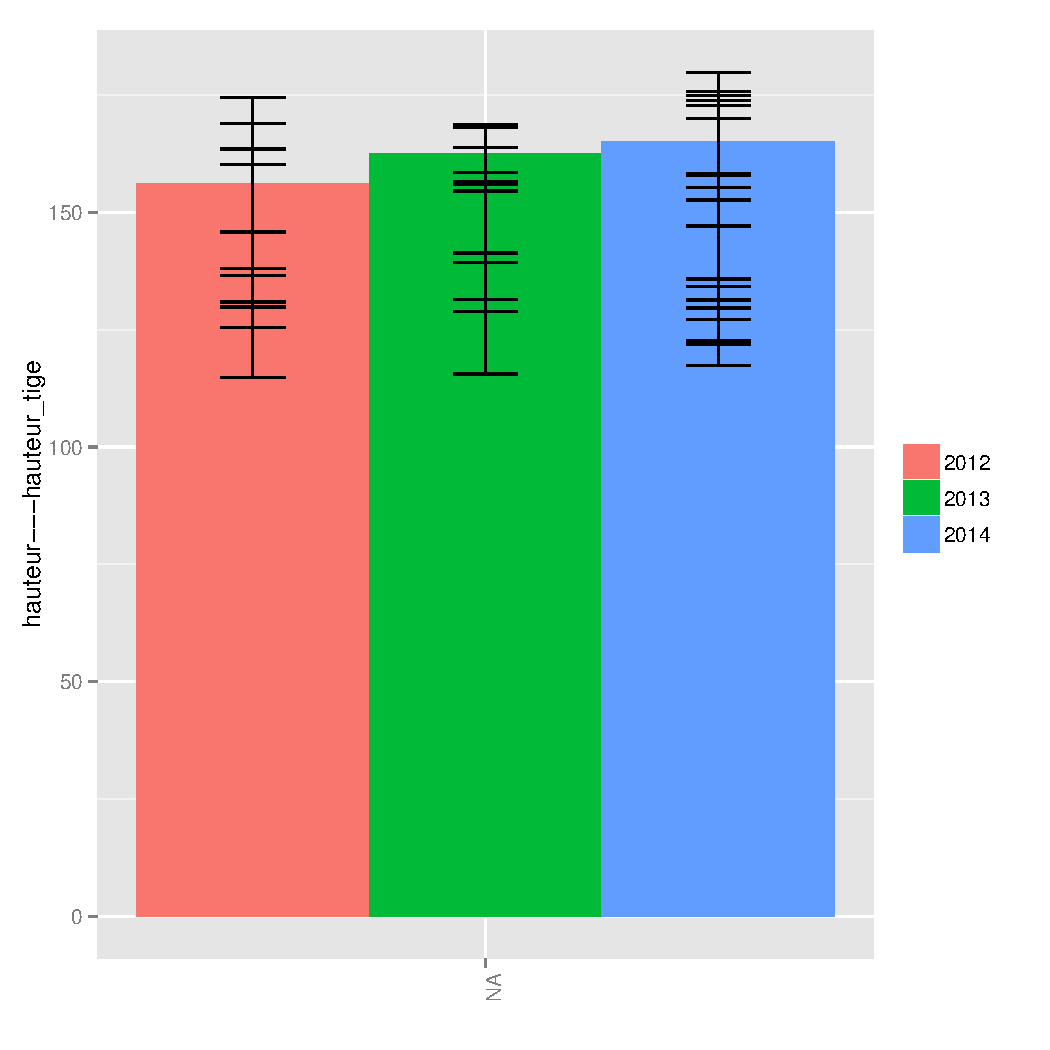
\includegraphics[width=.4\textwidth]{figures/shinemas2R_unnamed-chunk-71-1} 

}



\end{knitrout}
&
\begin{knitrout}
\definecolor{shadecolor}{rgb}{0.969, 0.969, 0.969}\color{fgcolor}

{\centering 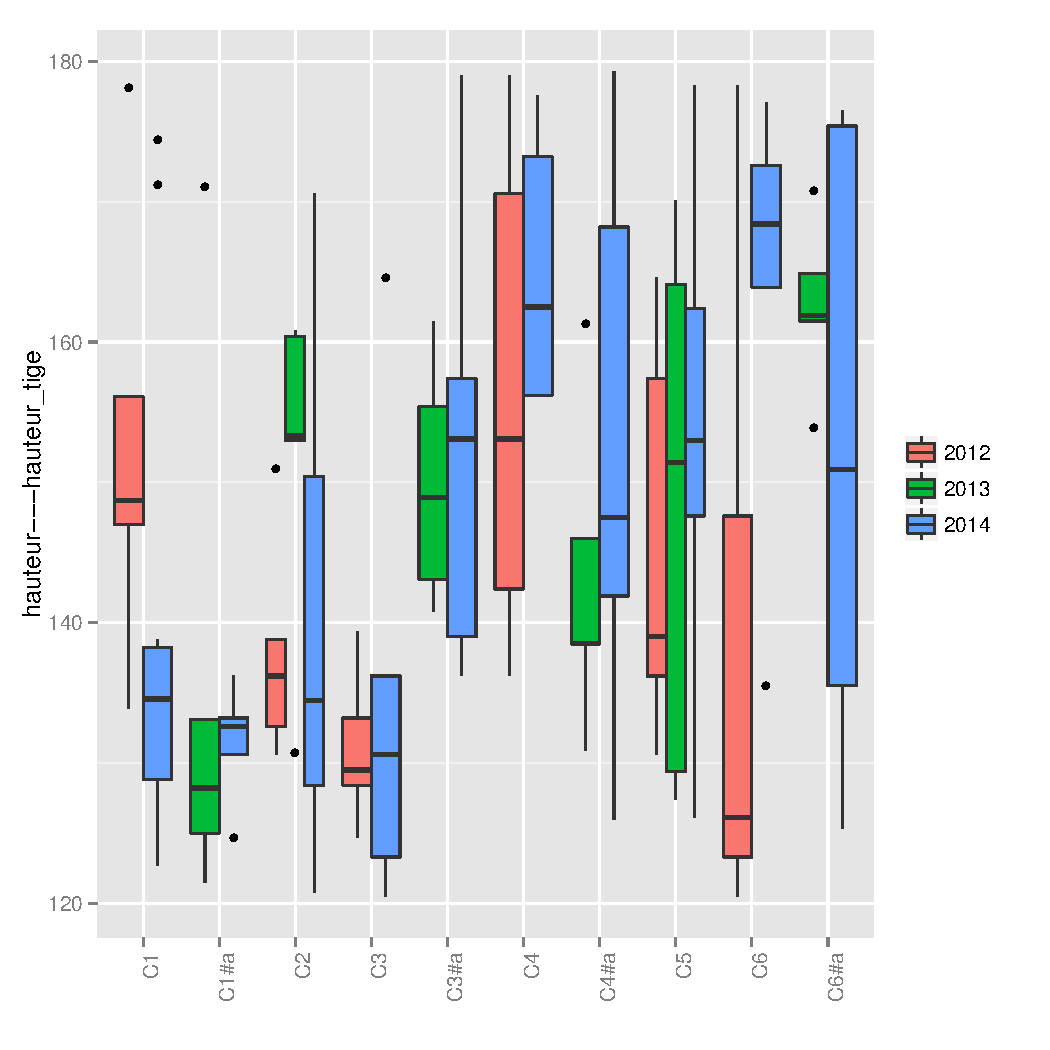
\includegraphics[width=.4\textwidth]{figures/shinemas2R_unnamed-chunk-72-1} 

}



\end{knitrout}
\\
\texttt{p\_cal\_ph\_int} & \\
\begin{knitrout}
\definecolor{shadecolor}{rgb}{0.969, 0.969, 0.969}\color{fgcolor}

{\centering 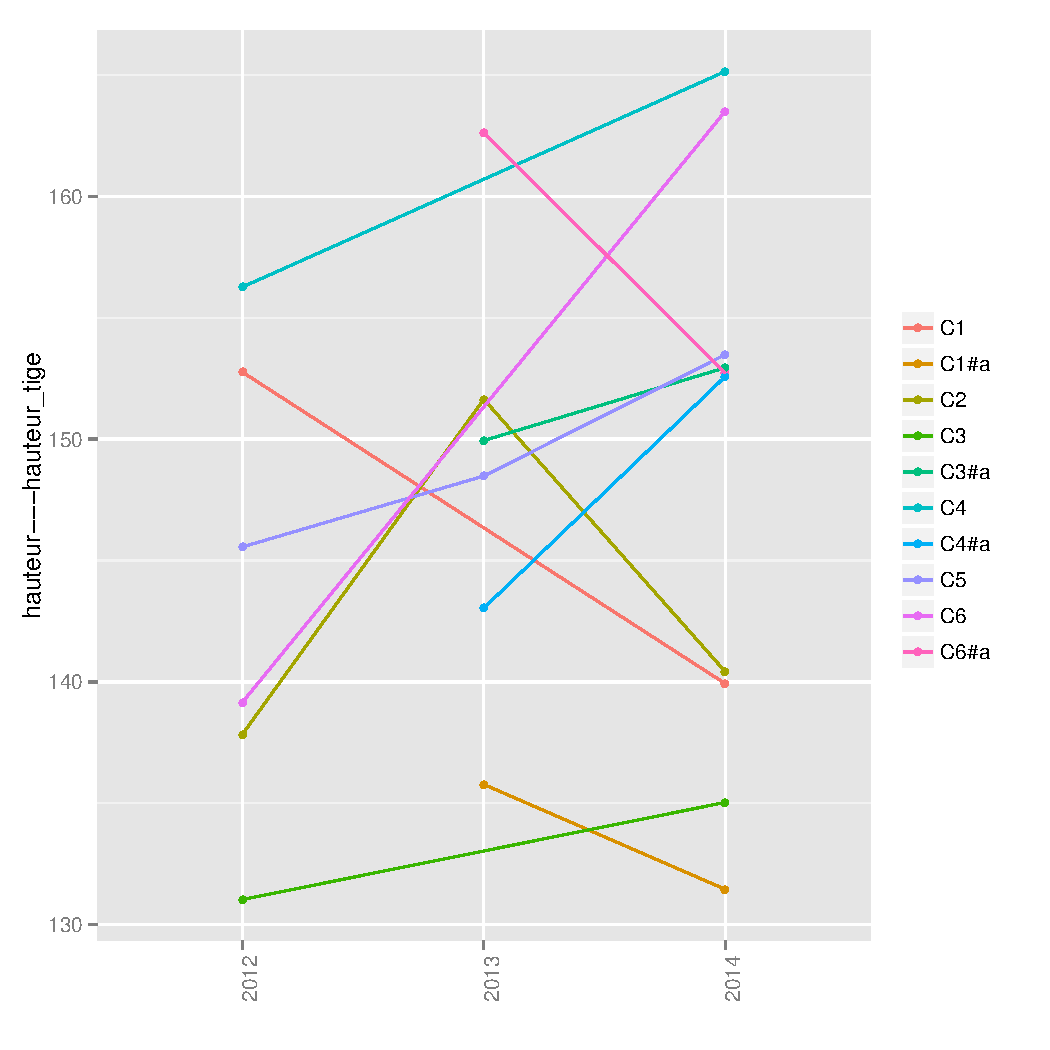
\includegraphics[width=.4\textwidth]{figures/shinemas2R_unnamed-chunk-73-1} 

}



\end{knitrout}
&
\\
\end{tabular}
\end{center}



For \texttt{ggplot.type = } \texttt{data-radar}, \texttt{data-biplot}, you may choose what you want in color (\texttt{in.col} argument).
The possible values for \texttt{in.col} are: \texttt{germplasm}, \texttt{year} and \texttt{person}.

\begin{knitrout}
\definecolor{shadecolor}{rgb}{0.969, 0.969, 0.969}\color{fgcolor}\begin{kframe}
\begin{alltt}
\hlkwd{names}\hlstd{(default_data_classic_ggplot}\hlopt{$}\hlstd{`data-radar`)}
\end{alltt}
\begin{verbatim}
## [1] "NA-year"      "NA-person"    "NA-germplasm"
\end{verbatim}
\end{kframe}
\end{knitrout}

For example,
\begin{knitrout}
\definecolor{shadecolor}{rgb}{0.969, 0.969, 0.969}\color{fgcolor}\begin{kframe}
\begin{alltt}
\hlstd{p_cal_rad_all} \hlkwb{=} \hlstd{default_data_classic_ggplot}\hlopt{$}\hlstd{`data-radar`}
\hlstd{p_cal_rad} \hlkwb{=} \hlstd{p_cal_rad_all}\hlopt{$}\hlstd{`NA-germplasm`}\hlopt{$}\hlstd{`x.axis-1|in.col-1`}
\end{alltt}
\end{kframe}
\end{knitrout}

For biplot, you must choose the pair of variables you wish, for example,
\begin{knitrout}
\definecolor{shadecolor}{rgb}{0.969, 0.969, 0.969}\color{fgcolor}\begin{kframe}
\begin{alltt}
\hlstd{p_cal_ph_sl_bip_all} \hlkwb{=} \hlstd{default_data_classic_ggplot}\hlopt{$}\hlstd{`data-biplot`}
\hlstd{p_cal_ph_sl_bip} \hlkwb{=} \hlstd{p_cal_ph_sl_bip_all}\hlopt{$}\hlstd{`NA-year`}
\hlstd{p_cal_ph_sl_bip} \hlkwb{=} \hlstd{p_cal_ph_sl_bip}\hlopt{$}\hlstd{`hauteur---hauteur_tige - poids_epis---poids_epis`}
\hlstd{p_cal_ph_sl_bip} \hlkwb{=} \hlstd{p_cal_ph_sl_bip}\hlopt{$}\hlstd{`x.axis-1|in.col-1`}
\end{alltt}
\end{kframe}
\end{knitrout}

\begin{center}
\begin{tabular}{cc}
\texttt{p\_cal\_rad} & \texttt{p\_cal\_ph\_sl\_bip} \\
\begin{knitrout}
\definecolor{shadecolor}{rgb}{0.969, 0.969, 0.969}\color{fgcolor}

{\centering 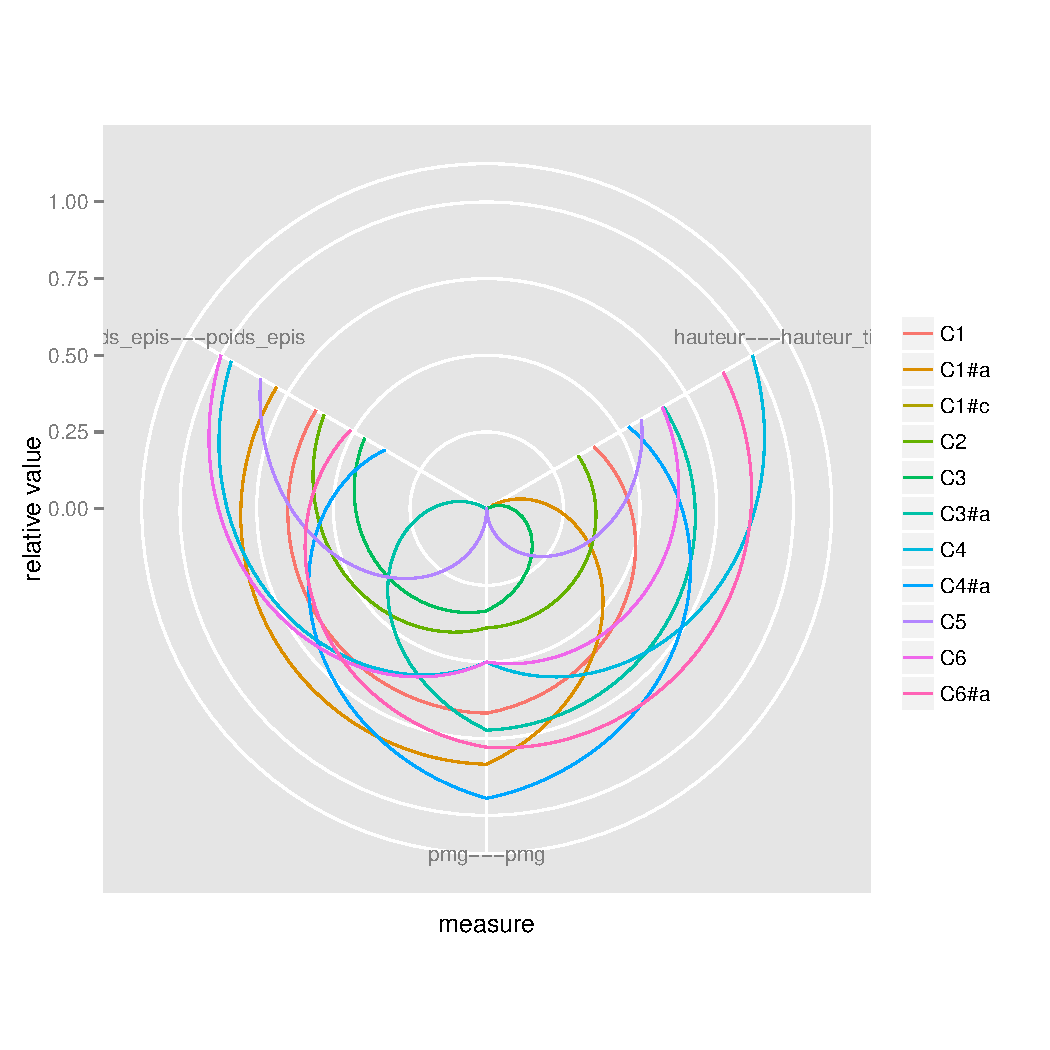
\includegraphics[width=.4\textwidth]{figures/shinemas2R_unnamed-chunk-77-1} 

}



\end{knitrout}
&
\begin{knitrout}
\definecolor{shadecolor}{rgb}{0.969, 0.969, 0.969}\color{fgcolor}

{\centering 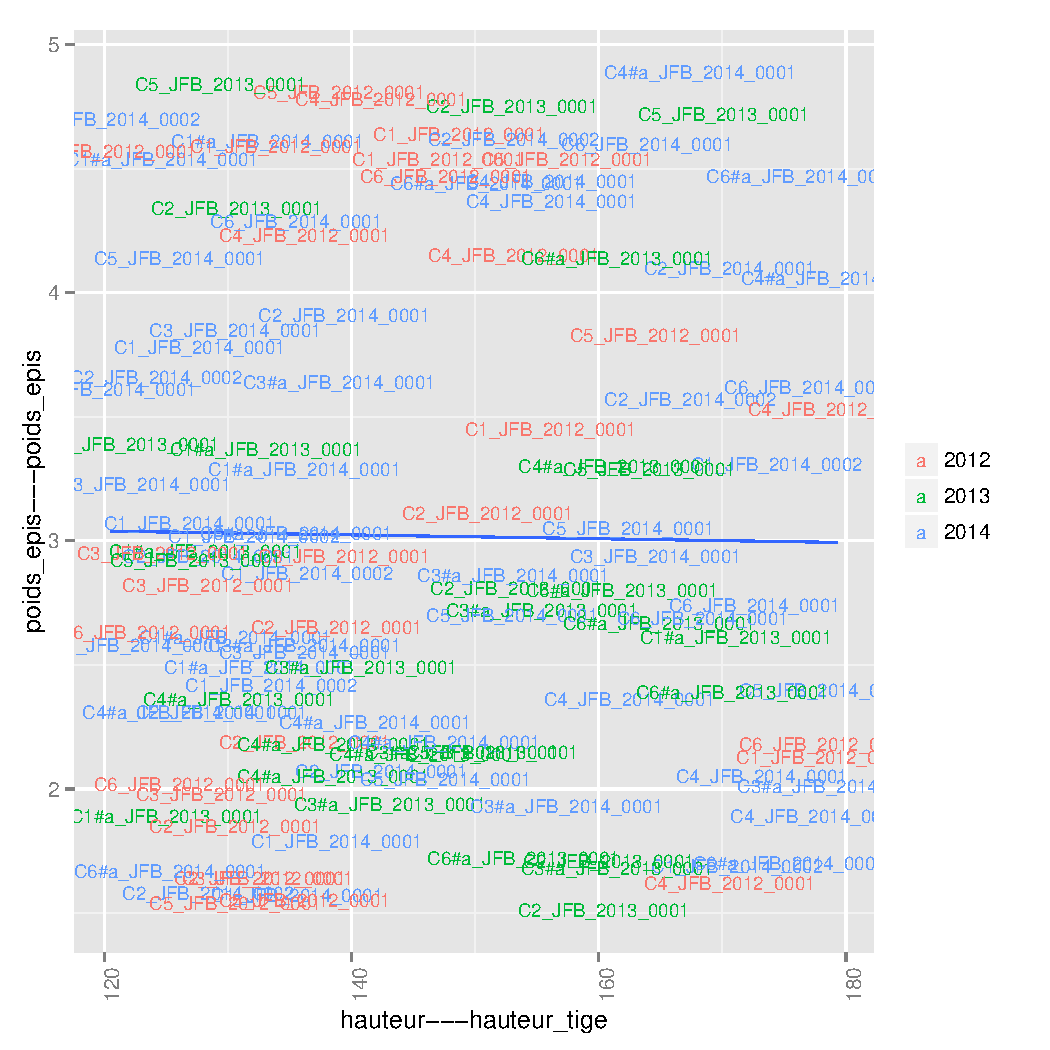
\includegraphics[width=.4\textwidth]{figures/shinemas2R_unnamed-chunk-78-1} 

}



\end{knitrout}
\\
\end{tabular}
\end{center}


\item Custom arguments 

According to \texttt{ggplot.type}, arguments can be customized:


\begin{center}
\begin{table}[H]
\begin{tabular}{ 
p{.2\textwidth} 
p{.1\textwidth} 
p{.4\textwidth}
ccccc 
}
\hline
argument & 
default value & 
description & 
\rotatebox{90}{\texttt{data-barplot}} &
\rotatebox{90}{\texttt{data-boxplot}} & 
\rotatebox{90}{\texttt{data-interaction}} & 
\rotatebox{90}{\texttt{data-radar}} & 
\rotatebox{90}{\texttt{data-biplot}} \\
\hline

\texttt{ggplot.on} & 
\texttt{"son"} & 
\texttt{"father"} or \texttt{"son"} depending on which seed-lot you want to plot.. &
X &
X &
X &
X &
X \\
\hline

\texttt{x.axis} & 
\texttt{NULL} & 
factor displayed on the \texttt{x.axis}	 of a plot: \texttt{"germplasm"}, \texttt{"year"} or \texttt{"person"} referring to the attributes of a seed-lots. If \texttt{NULL}, all the combinaison are done for \texttt{x.axis} and \texttt{in.col}. &
X &
X &
X &
  &
\\
\hline

\texttt{in.col} & 
\texttt{NULL} & 
display in color of a plot: \texttt{"germplasm"}, \texttt{"year"} or \texttt{"person"} referring to the attributes of a seed-lots. If \texttt{NULL}, \texttt{in.col} is not displayed. Note it is compulsory for data-biplot and data-radar as in these cases \texttt{x.axis} is not used. &
X &
X &
X &
X &
X \\
\hline

\texttt{nb\_parameters\_per} \texttt{\_plot\_x.axis} & 
\texttt{NULL} & 
the number of parameters per plot on \texttt{x.axis} argument &
X &
X &
X &
  &
\\
\hline

\texttt{nb\_parameters\_per} \texttt{\_plot\_in.col} & 
\texttt{NULL} & 
the number of parameters per plot for \texttt{in.col} argument &
X &
X &
X &
X &
X \\
\hline

\texttt{hide.labels.parts} & 
\texttt{"all"} & 
parts of the label hidden: \texttt{"germplasm"}, \texttt{"person"}, \texttt{"year"}, \texttt{"person:germplasm"}, \texttt{"year:germplasm"}, \texttt{"person:year"}, \texttt{"all"}. 
\texttt{"all"} means that no label is dispayed. 
If \texttt{NULL} labels are displayed. Labels are based on seed-lots names under the form \texttt{germplasm\_year\_person\_digit}.
For \texttt{"data-biplot"}, the default value is \texttt{NULL}.
For easier visualisation, digit is never displayed unless you choose \texttt{NULL}. &
  &
  &
  &
  &
X \\

\hline
\end{tabular}
\caption{Possible arguments regarding \texttt{ggplot.type}.
A cross (X) means that for a given \texttt{ggplot.type}, a given argument can be used.}
\label{custom.plot}
\end{table}
\end{center}

\end{itemize}

\item pies on network

\begin{itemize}

\item Default arguments

It is possible to add pies on seed-lots represented on a network.
The pie represent the distribution of a given variable for a given seed-lot.

In the following example, as we're working with encrypted data, \texttt{get.ggplot} reverse the transcription to query \BD~and encrypt again.

Note that this example is done on a little data set.
Indeed, the pies are drawn with a polygon which needs lots of points that take memory.

\begin{knitrout}
\definecolor{shadecolor}{rgb}{0.969, 0.969, 0.969}\color{fgcolor}\begin{kframe}
\begin{alltt}
\hlkwa{if}\hlstd{(use.get.data)\{}
        \hlstd{data_classic_bis} \hlkwb{=} \hlkwd{get.data}\hlstd{(}
                \hlkwc{db_user} \hlstd{= info_db}\hlopt{$}\hlstd{db_user,} \hlkwc{db_host} \hlstd{= info_db}\hlopt{$}\hlstd{db_host,} \hlcom{# db infos}
                \hlkwc{db_name} \hlstd{= info_db}\hlopt{$}\hlstd{db_name,} \hlkwc{db_password} \hlstd{= info_db}\hlopt{$}\hlstd{db_password,} \hlcom{# db infos}
                \hlkwc{query.type} \hlstd{=} \hlstr{"data-classic"}\hlstd{,} \hlcom{# data-classic query}
                \hlkwc{person.in} \hlstd{=} \hlstr{"OLR"}\hlstd{,} \hlcom{# person to keep}
                \hlkwc{filter.on} \hlstd{=} \hlstr{"father-son"}\hlstd{,} \hlcom{# filters on father AND son}
                \hlkwc{data.type} \hlstd{=} \hlstr{"relation"}\hlstd{,} \hlcom{# data linked to relation between seed-lots}
                \hlkwc{variable} \hlstd{=} \hlstr{"poids_epis"}\hlstd{,} \hlcom{# the variables to display}
                \hlkwc{project.in} \hlstd{=} \hlstr{"DEMO"} \hlcom{# the project }
                \hlstd{)}

        \hlstd{pn} \hlkwb{=} \hlkwd{get.ggplot}\hlstd{(}
                \hlstd{data_classic_bis,}
                \hlkwc{ggplot.type} \hlstd{=} \hlstr{"data-pie.on.network"}\hlstd{,}
                \hlkwc{vec_variables} \hlstd{=} \hlstr{"poids_epis---poids_epis"}\hlstd{,}
                \hlkwc{pie.size} \hlstd{=} \hlnum{.25}\hlstd{,}
                \hlkwc{hide.labels.parts} \hlstd{=} \hlstr{"person"}
                \hlstd{)}

\hlstd{\}} \hlkwa{else} \hlstd{\{}
        \hlcom{# 1. Query SHiNeMaS ...}
        \hlcom{# 2. Set up data set ...}
        \hlcom{# |==========================================================| 100%}
        \hlkwd{load}\hlstd{(}\hlstr{"./data/data_classic_bis.RData"}\hlstd{)}

        \hlcom{# 1. Query SHiNeMaS ...}
        \hlcom{# 2. Create network matrix ...}
        \hlcom{# 3. Link information to vertex and edges ...}
        \hlkwd{load}\hlstd{(}\hlstr{"./data/pn.RData"}\hlstd{)}
        \hlstd{\}}
\end{alltt}
\end{kframe}
\end{knitrout}

As we're working on one person, we set \texttt{hide.labels.parts = "person"}.

The result is divided into two plots: the empty network and the network with the pies.

\begin{knitrout}
\definecolor{shadecolor}{rgb}{0.969, 0.969, 0.969}\color{fgcolor}\begin{kframe}
\begin{alltt}
\hlkwd{names}\hlstd{(pn}\hlopt{$}\hlstd{`data-pie.on.network`)}
\end{alltt}
\begin{verbatim}
## [1] "poids_epis---poids_epis"
\end{verbatim}
\begin{alltt}
\hlstd{p1} \hlkwb{=} \hlstd{pn}\hlopt{$}\hlstd{`data-pie.on.network`}\hlopt{$}\hlstd{`poids_epis---poids_epis`}\hlopt{$}\hlstd{network}
\hlstd{p2} \hlkwb{=} \hlstd{pn}\hlopt{$}\hlstd{`data-pie.on.network`}\hlopt{$}\hlstd{`poids_epis---poids_epis`}\hlopt{$}\hlstd{pie.on.network}
\end{alltt}
\end{kframe}
\end{knitrout}

\begin{center}
\begin{tabular}{c}
\texttt{p1}\\
\begin{knitrout}
\definecolor{shadecolor}{rgb}{0.969, 0.969, 0.969}\color{fgcolor}

{\centering 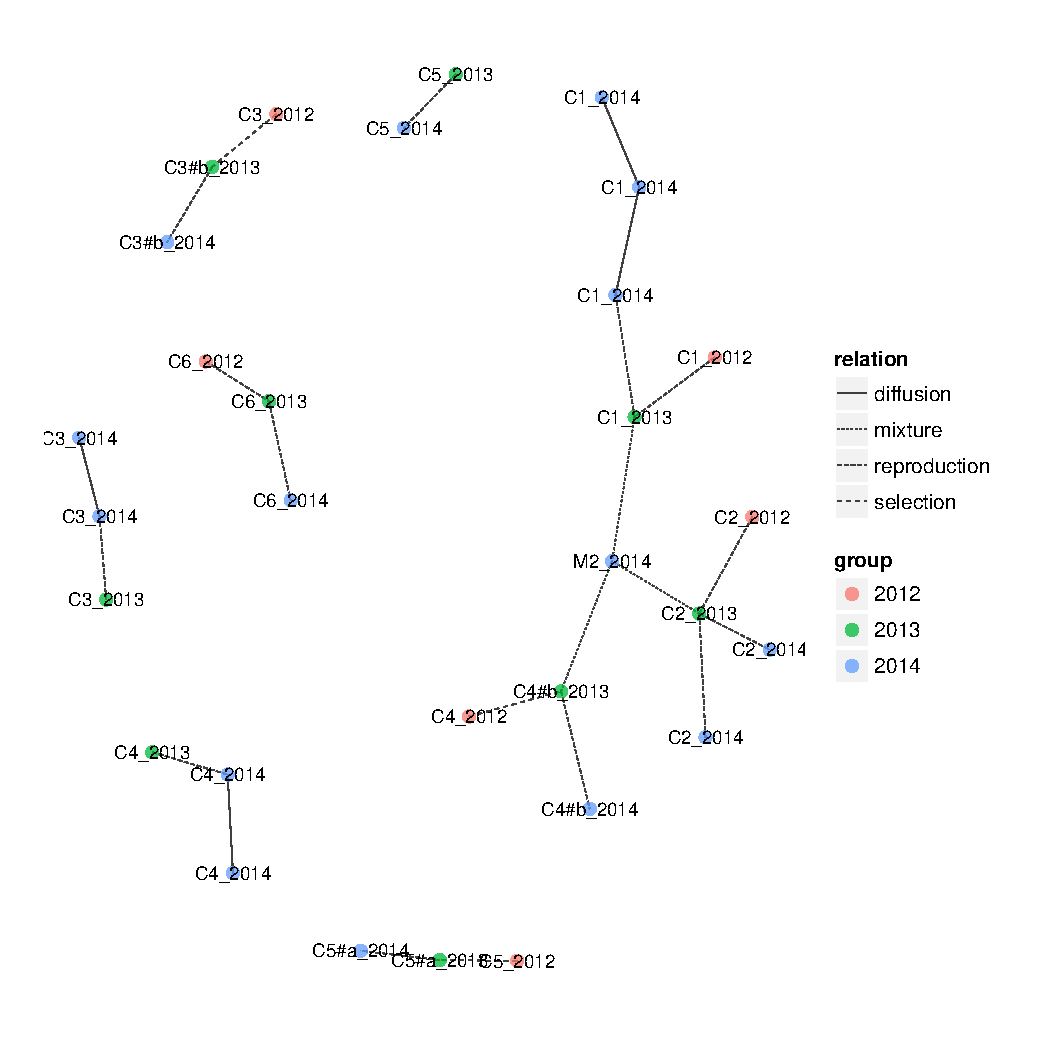
\includegraphics[width=.6\textwidth]{figures/shinemas2R_unnamed-chunk-81-1} 

}



\end{knitrout}
\\
\texttt{p2}\\
\begin{knitrout}
\definecolor{shadecolor}{rgb}{0.969, 0.969, 0.969}\color{fgcolor}

{\centering 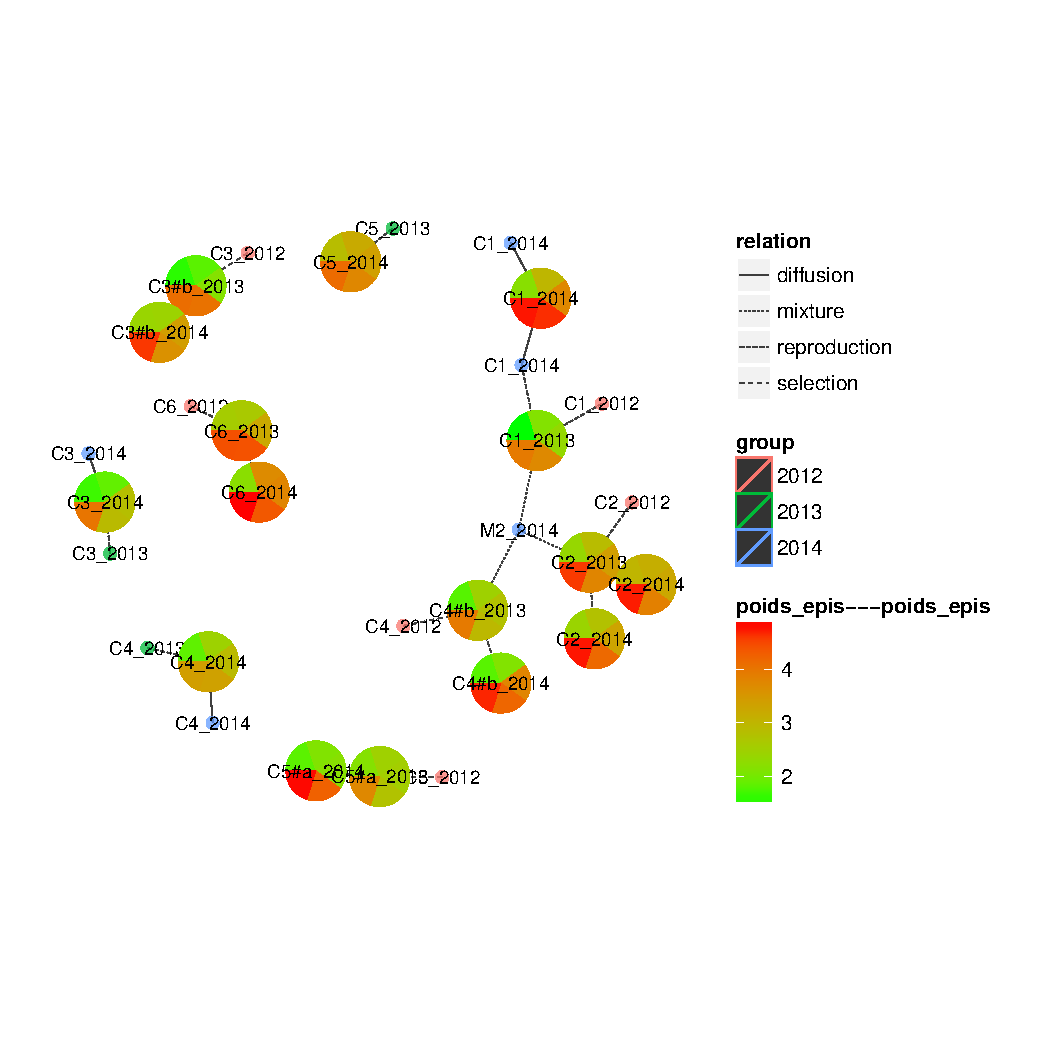
\includegraphics[width=.8\textwidth]{figures/shinemas2R_unnamed-chunk-82-1} 

}



\end{knitrout}
\\
\end{tabular}
\end{center}

\item Custom arguments

Arguments can be customized related to network plots (Table \ref{custom.network}).

\end{itemize}


\item pies on map

\begin{itemize}

\item Default arguments

\texttt{get.data} is called to get the coordinates data.

\begin{knitrout}
\definecolor{shadecolor}{rgb}{0.969, 0.969, 0.969}\color{fgcolor}\begin{kframe}
\begin{alltt}
\hlkwa{if}\hlstd{(use.get.data)\{}
        \hlstd{data_classic_ter} \hlkwb{=} \hlkwd{get.data}\hlstd{(}
                \hlkwc{db_user} \hlstd{= info_db}\hlopt{$}\hlstd{db_user,} \hlkwc{db_host} \hlstd{= info_db}\hlopt{$}\hlstd{db_host,} \hlcom{# db infos}
                \hlkwc{db_name} \hlstd{= info_db}\hlopt{$}\hlstd{db_name,} \hlkwc{db_password} \hlstd{= info_db}\hlopt{$}\hlstd{db_password,} \hlcom{# db infos}
                \hlkwc{query.type} \hlstd{=} \hlstr{"data-classic"}\hlstd{,} \hlcom{# data-classic query}
                \hlkwc{germplasm.in} \hlstd{=} \hlstr{"C1"}\hlstd{,} \hlcom{# germplasm to keep}
                \hlkwc{person.in} \hlstd{=} \hlkwd{c}\hlstd{(}\hlstr{"OLR"}\hlstd{,} \hlstr{"MLN"}\hlstd{,} \hlstr{"JFB"}\hlstd{),} \hlcom{# person to keep}
                \hlkwc{filter.on} \hlstd{=} \hlstr{"father-son"}\hlstd{,} \hlcom{# filters on father AND son}
                \hlkwc{data.type} \hlstd{=} \hlstr{"relation"}\hlstd{,} \hlcom{# data linked to relation between seed-lots}
                \hlkwc{variable} \hlstd{=} \hlstr{"poids_epis"}\hlstd{,} \hlcom{# the variables to display}
                \hlkwc{project.in} \hlstd{=} \hlstr{"DEMO"} \hlcom{# the project}
                \hlstd{)}

        \hlstd{pm} \hlkwb{=} \hlkwd{get.ggplot}\hlstd{(}
                \hlstd{data_classic_ter,}
                \hlkwc{ggplot.type} \hlstd{=} \hlstr{"data-pie.on.map"}\hlstd{,}
                \hlkwc{vec_variables} \hlstd{=} \hlstr{"poids_epis---poids_epis"}
                \hlstd{)}
\hlstd{\}} \hlkwa{else} \hlstd{\{}
        \hlkwd{load}\hlstd{(}\hlstr{"./data/data_classic_ter.RData"}\hlstd{)}
        \hlkwd{load}\hlstd{(}\hlstr{"./data/pm.RData"}\hlstd{)}
        \hlstd{\}}

\hlkwd{names}\hlstd{(pm}\hlopt{$}\hlstd{`data-pie.on.map`)}
\end{alltt}
\begin{verbatim}
## [1] "poids_epis---poids_epis"
\end{verbatim}
\end{kframe}
\end{knitrout}

You can get the default ggplot (\texttt{p}) or customized it (\texttt{p\_bis}):

\begin{knitrout}
\definecolor{shadecolor}{rgb}{0.969, 0.969, 0.969}\color{fgcolor}\begin{kframe}
\begin{alltt}
\hlstd{p} \hlkwb{=} \hlstd{pm}\hlopt{$}\hlstd{`data-pie.on.map`}\hlopt{$}\hlstd{`poids_epis---poids_epis`}\hlopt{$}\hlstd{`map-[2013]`}

\hlstd{p_bis} \hlkwb{=} \hlstd{p} \hlopt{+}
        \hlkwd{ggtitle}\hlstd{(}\hlstr{"spike_weight in 2011"}\hlstd{)} \hlopt{+} \hlcom{# change the title}
        \hlkwd{theme}\hlstd{(}\hlkwc{legend.title}\hlstd{=}\hlkwd{element_blank}\hlstd{())} \hlcom{# delete the name of the legend}
\end{alltt}
\end{kframe}
\end{knitrout}

\begin{center}
\begin{tabular}{cc}
\texttt{p} & \texttt{p\_bis} \\
\begin{knitrout}
\definecolor{shadecolor}{rgb}{0.969, 0.969, 0.969}\color{fgcolor}

{\centering 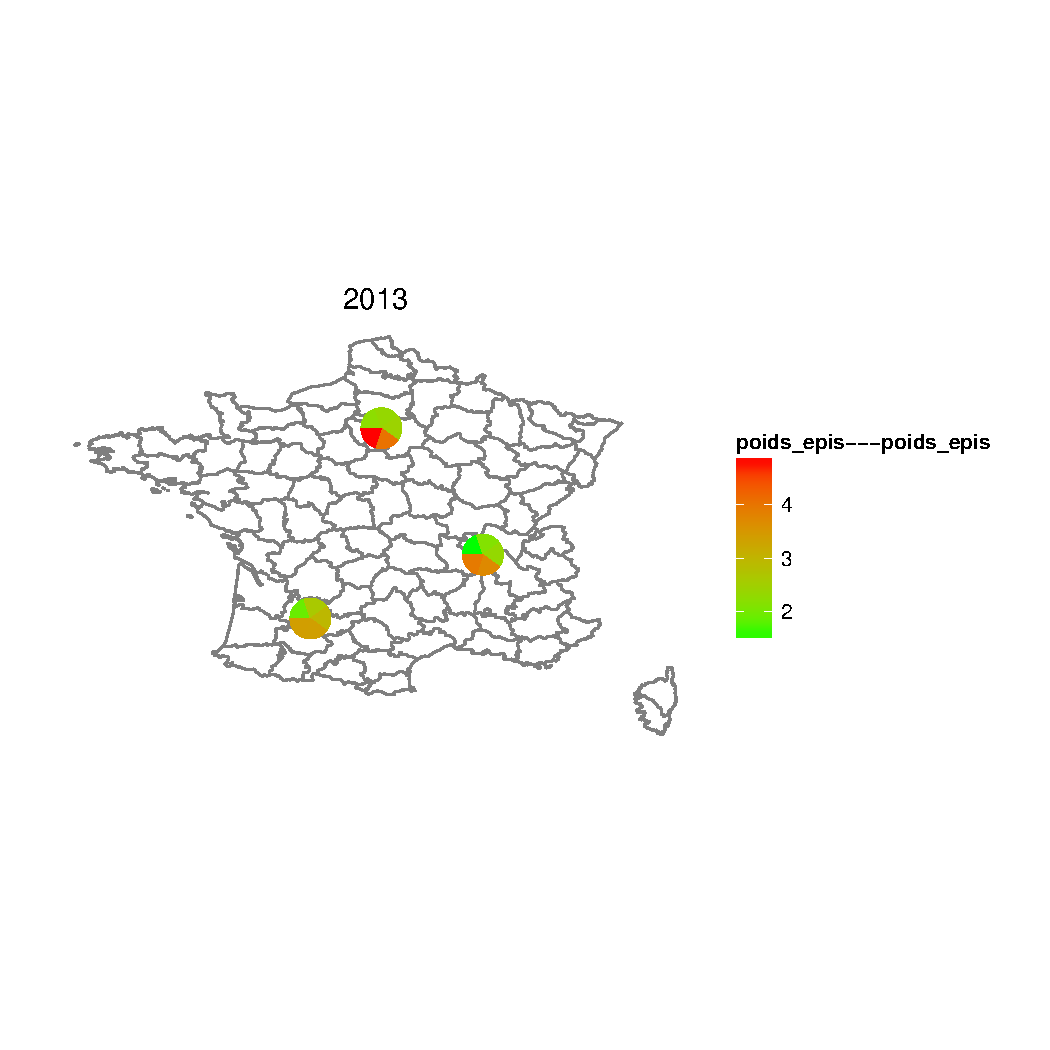
\includegraphics[width=.4\textwidth]{figures/shinemas2R_unnamed-chunk-85-1} 

}



\end{knitrout}
&
\begin{knitrout}
\definecolor{shadecolor}{rgb}{0.969, 0.969, 0.969}\color{fgcolor}

{\centering 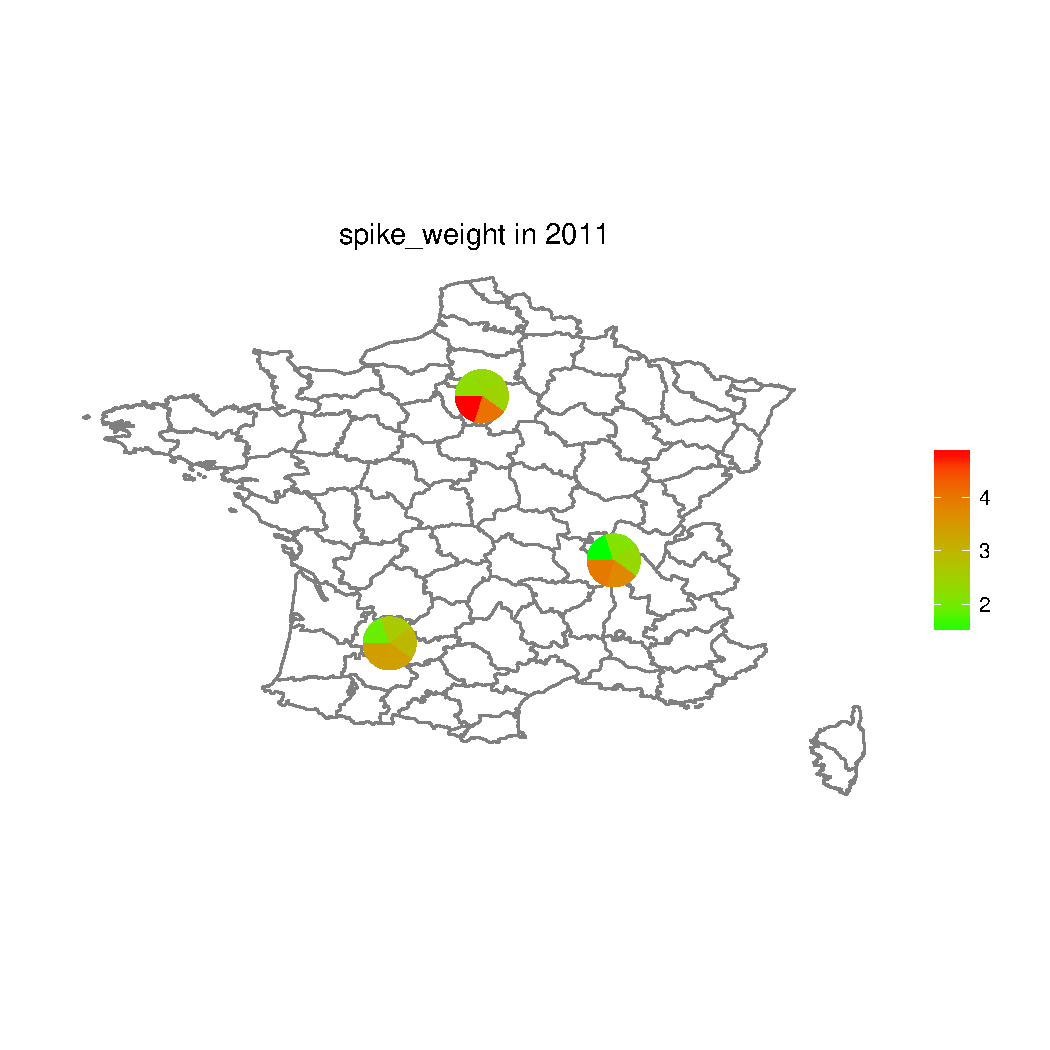
\includegraphics[width=.4\textwidth]{figures/shinemas2R_unnamed-chunk-86-1} 

}



\end{knitrout}
\\
\end{tabular}
\end{center}


\item Custom arguments

Arguments can be customed related to map plots (Table \ref{custom.map}).

For \texttt{data-pie.on.map}, it is also possible to choose \texttt{x.axis} in order to get a map for each \texttt{year} or each \texttt{germplasm}.

In the example, as \texttt{data\_classic} is done on one germplasm (C1), \texttt{x.axis = year} has been chosen (default argument).

\end{itemize}

\end{itemize}

\subsubsection{ggplots for \texttt{data-S} }

\begin{knitrout}
\definecolor{shadecolor}{rgb}{0.969, 0.969, 0.969}\color{fgcolor}\begin{kframe}
\begin{alltt}
\hlstd{default_data_S_ggplot} \hlkwb{=} \hlkwd{get.ggplot}\hlstd{(}
        \hlstd{data_S,}
        \hlkwc{vec_variables} \hlstd{= plot_vec_variables,}
        \hlkwc{nb_parameters_per_plot_x.axis} \hlstd{=} \hlnum{5}
        \hlstd{)}
\end{alltt}


{\ttfamily\noindent\itshape\color{messagecolor}{\#\# As ggplot.type is NULL, ggplot.Type is set to data-barplot, data-boxplot, data-interaction, data-radar, data-biplot\\\#\# As ggplot.type is NULL and data come from "{}data-S"{} or "{}data-SR"{}, ggplot.type is set to "{}data-barplot"{}, "{}data-boxplot"{}, "{}data-interaction"{}.\\\#\# With "{}data-S"{} and "{}data-SR"{}, in.col and x.axis are set automaticaly.}}\begin{verbatim}
## [1] "A Virer quand les données seront propres dans get.data"
## [1] "A Virer quand les données seront propres dans get.data"
## [1] "A Virer quand les données seront propres dans get.data"
\end{verbatim}
\end{kframe}
\end{knitrout}

By default, the following plots are done with \texttt{x.axis} and \texttt{in.col} (you can not change it).
Note that \texttt{NA} are put when there are no data for \texttt{bouquet} AND \texttt{vrac} (i.e. nothing is displayed).

\begin{knitrout}
\definecolor{shadecolor}{rgb}{0.969, 0.969, 0.969}\color{fgcolor}\begin{kframe}
\begin{alltt}
\hlkwd{names}\hlstd{(default_data_S_ggplot)}
\end{alltt}
\begin{verbatim}
## [1] "data-barplot"     "data-boxplot"     "data-interaction"
\end{verbatim}
\end{kframe}
\end{knitrout}

which correpond to ggplot.type arguments as explained in the previous section.

\begin{itemize}

\item For barplot:
\begin{knitrout}
\definecolor{shadecolor}{rgb}{0.969, 0.969, 0.969}\color{fgcolor}\begin{kframe}
\begin{alltt}
\hlstd{p_S_sw_bar_all} \hlkwb{=} \hlstd{default_data_S_ggplot}\hlopt{$}\hlstd{`data-barplot`}
\hlstd{p_S_sw_bar} \hlkwb{=} \hlstd{p_S_sw_bar_all}\hlopt{$}\hlstd{`pmg---pmg`}\hlopt{$}\hlstd{`x.axis-1|in.col-1`}
\end{alltt}
\end{kframe}
\end{knitrout}

\item For boxplot:
\begin{knitrout}
\definecolor{shadecolor}{rgb}{0.969, 0.969, 0.969}\color{fgcolor}\begin{kframe}
\begin{alltt}
\hlstd{p_S_sw_box_all} \hlkwb{=} \hlstd{default_data_S_ggplot}\hlopt{$}\hlstd{`data-boxplot`}
\hlstd{p_S_sw_box} \hlkwb{=} \hlstd{p_S_sw_box_all}\hlopt{$}\hlstd{`pmg---pmg`}\hlopt{$}\hlstd{`x.axis-1|in.col-1`}
\end{alltt}
\end{kframe}
\end{knitrout}

\item For interaction plot:
\begin{knitrout}
\definecolor{shadecolor}{rgb}{0.969, 0.969, 0.969}\color{fgcolor}\begin{kframe}
\begin{alltt}
\hlstd{p_S_sw_int_all} \hlkwb{=} \hlstd{default_data_S_ggplot}\hlopt{$}\hlstd{`data-interaction`}
\hlstd{p_S_sw_int} \hlkwb{=} \hlstd{p_S_sw_int_all}\hlopt{$}\hlstd{`pmg---pmg`}\hlopt{$}\hlstd{`x.axis-1|in.col-1`}
\end{alltt}
\end{kframe}
\end{knitrout}

\end{itemize}



\begin{center}
\begin{tabular}{cc}
\texttt{p\_S\_sw\_bar} & \texttt{p\_S\_sw\_box} \\
\begin{knitrout}
\definecolor{shadecolor}{rgb}{0.969, 0.969, 0.969}\color{fgcolor}

{\centering 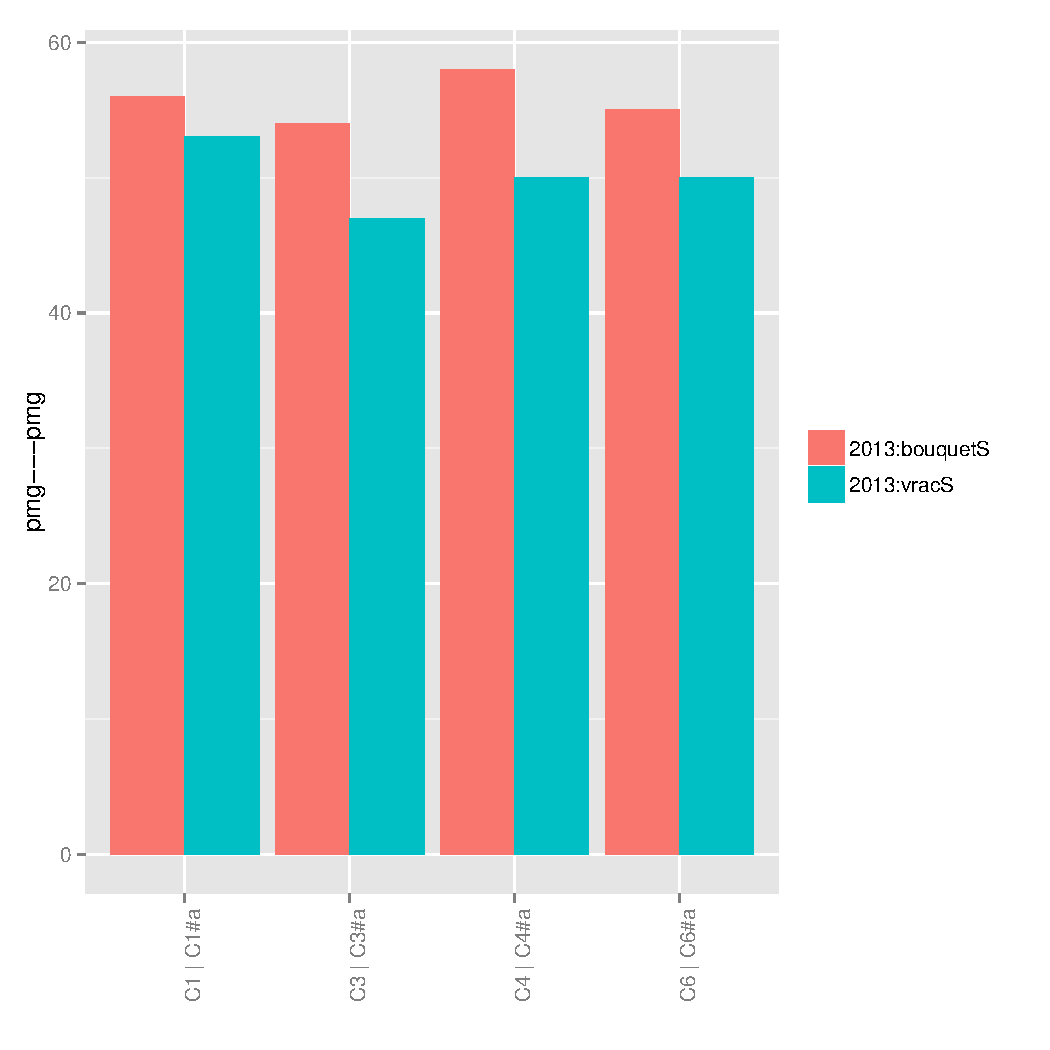
\includegraphics[width=.4\textwidth]{figures/shinemas2R_unnamed-chunk-92-1} 

}



\end{knitrout}
&
\begin{knitrout}
\definecolor{shadecolor}{rgb}{0.969, 0.969, 0.969}\color{fgcolor}

{\centering 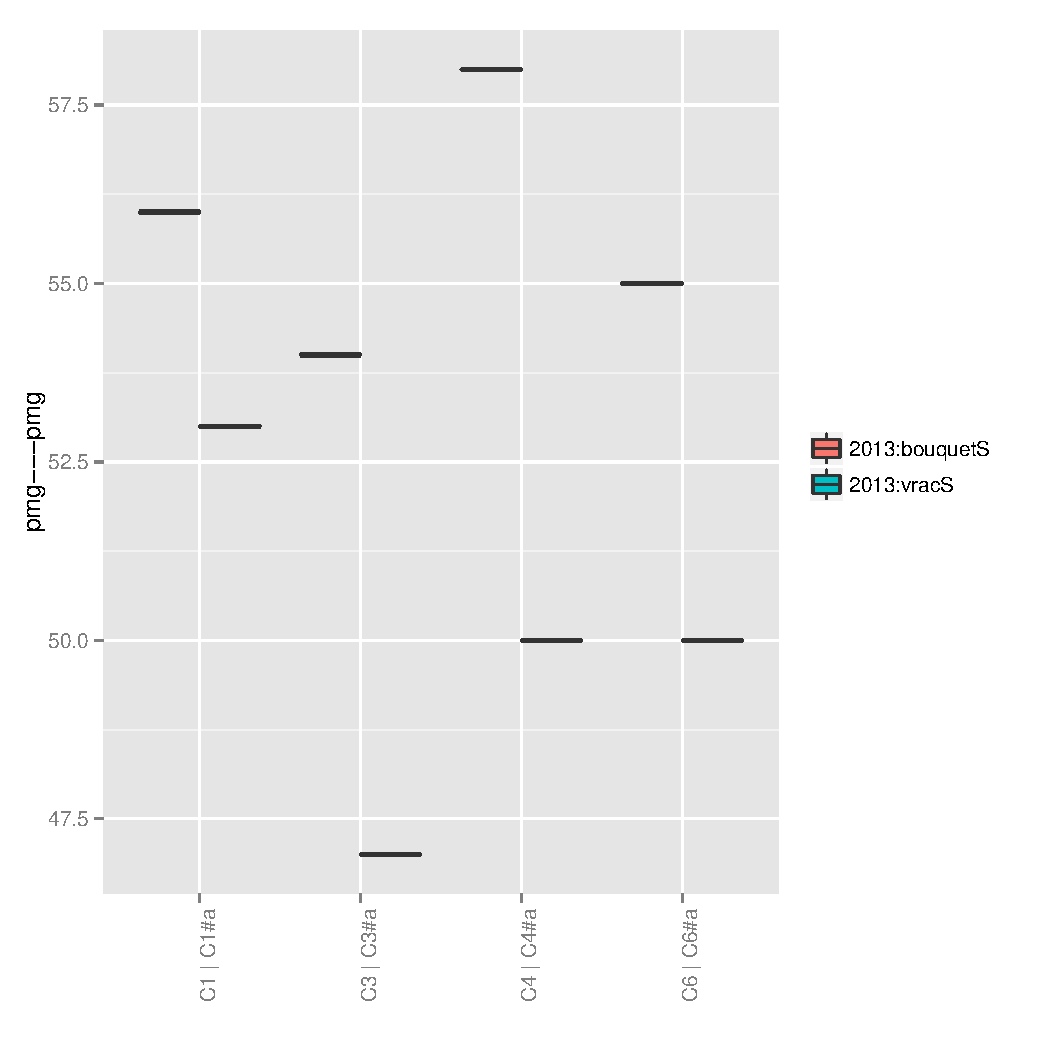
\includegraphics[width=.4\textwidth]{figures/shinemas2R_unnamed-chunk-93-1} 

}



\end{knitrout}
\\
\texttt{p\_S\_sw\_int} & \\
\begin{knitrout}
\definecolor{shadecolor}{rgb}{0.969, 0.969, 0.969}\color{fgcolor}

{\centering 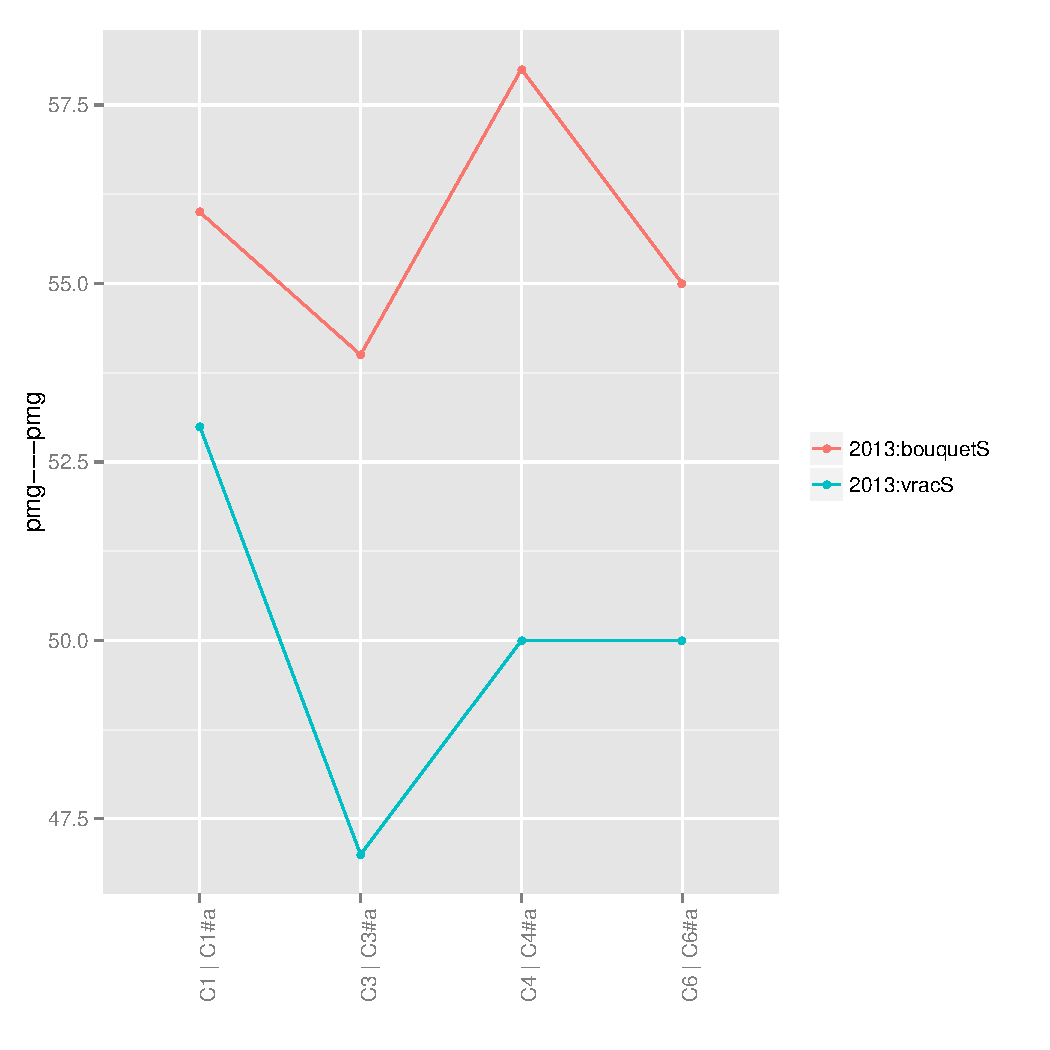
\includegraphics[width=.4\textwidth]{figures/shinemas2R_unnamed-chunk-94-1} 

}



\end{knitrout}
&
\\
\end{tabular}
\end{center}

It is possible to customize the plots as presented in Table \ref{custom.plot}.

\subsubsection{ggplots for \texttt{data-SR} }

\begin{knitrout}
\definecolor{shadecolor}{rgb}{0.969, 0.969, 0.969}\color{fgcolor}\begin{kframe}
\begin{alltt}
\hlstd{default_data_SR_ggplot} \hlkwb{=} \hlkwd{get.ggplot}\hlstd{(}
        \hlstd{data_SR,}
        \hlkwc{vec_variables} \hlstd{= plot_vec_variables,}
        \hlkwc{nb_parameters_per_plot_x.axis} \hlstd{=} \hlnum{5}
        \hlstd{)}
\end{alltt}


{\ttfamily\noindent\itshape\color{messagecolor}{\#\# As ggplot.type is NULL, ggplot.Type is set to data-barplot, data-boxplot, data-interaction, data-radar, data-biplot\\\#\# As ggplot.type is NULL and data come from "{}data-S"{} or "{}data-SR"{}, ggplot.type is set to "{}data-barplot"{}, "{}data-boxplot"{}, "{}data-interaction"{}.\\\#\# With "{}data-S"{} and "{}data-SR"{}, in.col and x.axis are set automaticaly.}}\begin{verbatim}
## [1] "A Virer quand les données seront propres dans get.data"
## [1] "A Virer quand les données seront propres dans get.data"
## [1] "A Virer quand les données seront propres dans get.data"
\end{verbatim}
\end{kframe}
\end{knitrout}

By default, the following plots are done with \texttt{x.axis} and \texttt{in.col} (you can not change it).
Note that \texttt{NA} are put when there are no data for \texttt{bouquet} AND \texttt{vrac} (i.e. nothing is displayed).

\begin{knitrout}
\definecolor{shadecolor}{rgb}{0.969, 0.969, 0.969}\color{fgcolor}\begin{kframe}
\begin{alltt}
\hlkwd{names}\hlstd{(default_data_SR_ggplot)}
\end{alltt}
\begin{verbatim}
## [1] "data-barplot"     "data-boxplot"     "data-interaction"
\end{verbatim}
\end{kframe}
\end{knitrout}

which correpond to ggplot.type arguments as explained in the previsou section.

\begin{itemize}
\item For barplot:
\begin{knitrout}
\definecolor{shadecolor}{rgb}{0.969, 0.969, 0.969}\color{fgcolor}\begin{kframe}
\begin{alltt}
\hlstd{p_SR_sw_bar_all} \hlkwb{=} \hlstd{default_data_SR_ggplot}\hlopt{$}\hlstd{`data-barplot`}
\hlstd{p_SR_sw_bar} \hlkwb{=} \hlstd{p_SR_sw_bar_all}\hlopt{$}\hlstd{`poids_epis---poids_epis`}\hlopt{$}\hlstd{`x.axis-1|in.col-1`}
\end{alltt}
\end{kframe}
\end{knitrout}

\item For boxplot:
\begin{knitrout}
\definecolor{shadecolor}{rgb}{0.969, 0.969, 0.969}\color{fgcolor}\begin{kframe}
\begin{alltt}
\hlstd{p_SR_sw_box_all} \hlkwb{=} \hlstd{default_data_SR_ggplot}\hlopt{$}\hlstd{`data-boxplot`}
\hlstd{p_SR_sw_box} \hlkwb{=} \hlstd{p_SR_sw_box_all}\hlopt{$}\hlstd{`poids_epis---poids_epis`}\hlopt{$}\hlstd{`x.axis-1|in.col-1`}
\end{alltt}
\end{kframe}
\end{knitrout}

\item For interaction plot:
\begin{knitrout}
\definecolor{shadecolor}{rgb}{0.969, 0.969, 0.969}\color{fgcolor}\begin{kframe}
\begin{alltt}
\hlstd{p_SR_sw_int_all} \hlkwb{=} \hlstd{default_data_SR_ggplot}\hlopt{$}\hlstd{`data-interaction`}
\hlstd{p_SR_sw_int} \hlkwb{=} \hlstd{p_SR_sw_int_all}\hlopt{$}\hlstd{`poids_epis---poids_epis`}\hlopt{$}\hlstd{`x.axis-1|in.col-1`}
\end{alltt}
\end{kframe}
\end{knitrout}

\end{itemize}

\begin{center}
\begin{tabular}{cc}
\texttt{p\_SR\_sw\_bar} & \texttt{p\_SR\_sw\_box} \\
\begin{knitrout}
\definecolor{shadecolor}{rgb}{0.969, 0.969, 0.969}\color{fgcolor}

{\centering 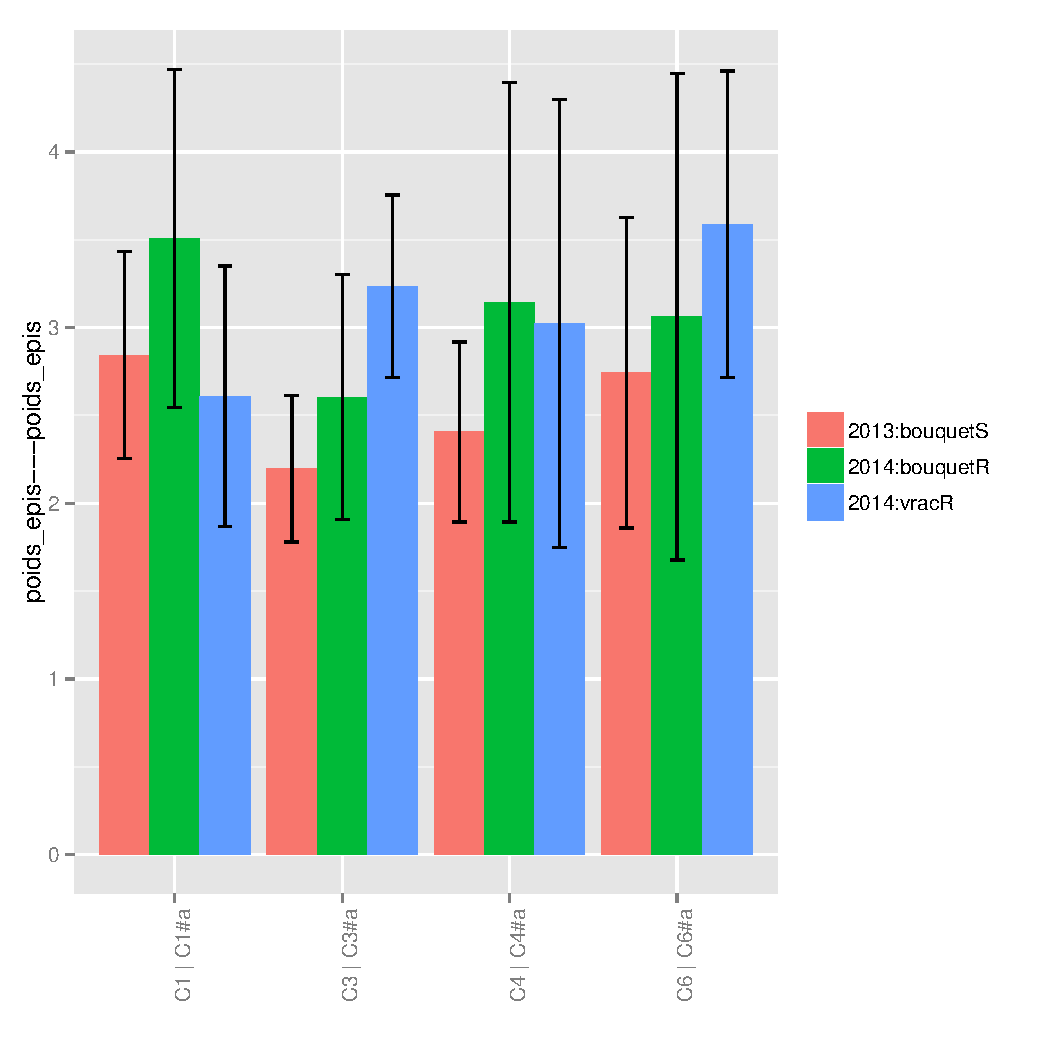
\includegraphics[width=.4\textwidth]{figures/shinemas2R_unnamed-chunk-100-1} 

}



\end{knitrout}
&
\begin{knitrout}
\definecolor{shadecolor}{rgb}{0.969, 0.969, 0.969}\color{fgcolor}

{\centering 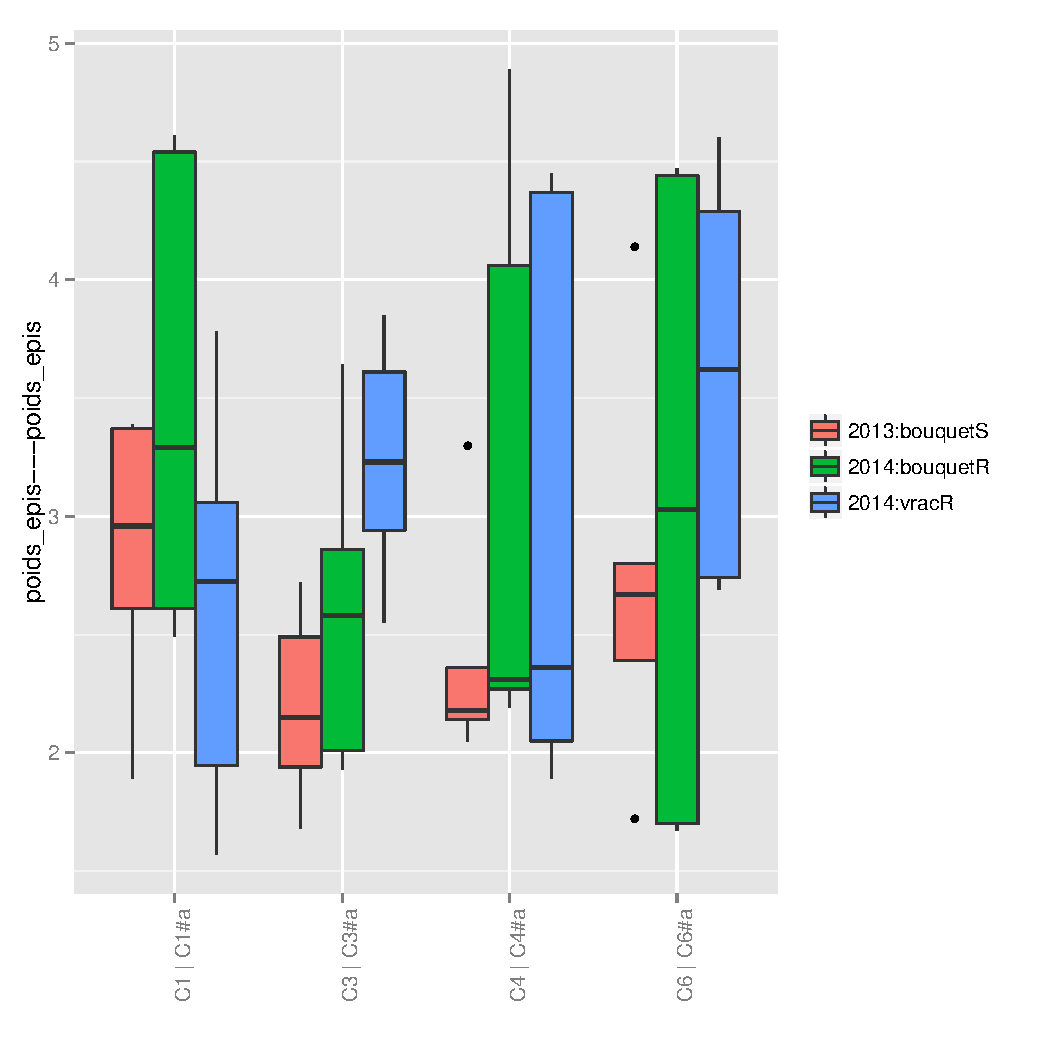
\includegraphics[width=.4\textwidth]{figures/shinemas2R_unnamed-chunk-101-1} 

}



\end{knitrout}
\\
\texttt{p\_SR\_sw\_int} & \\
\begin{knitrout}
\definecolor{shadecolor}{rgb}{0.969, 0.969, 0.969}\color{fgcolor}

{\centering 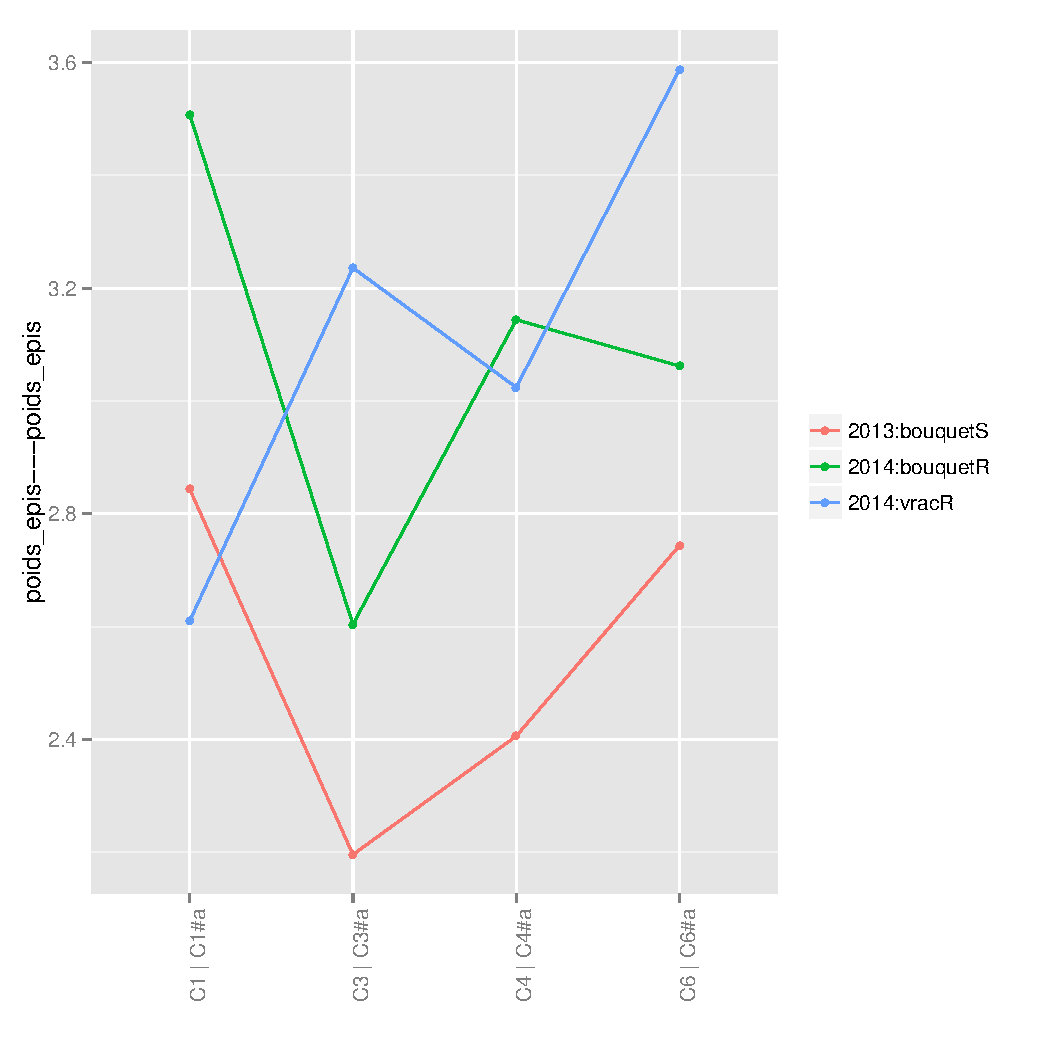
\includegraphics[width=.4\textwidth]{figures/shinemas2R_unnamed-chunk-102-1} 

}



\end{knitrout}
&
\\
\end{tabular}
\end{center}


It is possible to customize the plots as presented in Table \ref{custom.plot}.


\subsection{Get the tables}

From the data, to get the tables, use the function \texttt{get.table}.

First of all ,you need to choose

\begin{itemize}
\item on which data set you get the ggplots.
This can be done with \texttt{correlated\_group} having the following argument:
\begin{itemize}
\item \texttt{NULL}, the default argument (\texttt{shinemas2R::get.data()\$data\$data})
\item the name of a given \texttt{correlation\_group} (\texttt{shinemas2R::get.data()\$data\$data.with.correlated.variables})
\end{itemize}

\item if you want to merge germplasm name and selection name with the argument \texttt{merge\_g\_and\_s} which is \texttt{TRUE} by default
\end{itemize}


Five types of tables can be displayed according to \texttt{table.type} argument :

\begin{center}
\begin{tabular}{ll}
\hline
\texttt{table.type} & description \\
\hline

\texttt{"raw"} & display raw data. Useful with text for example \\
\hline

\texttt{"mean"} & displayed for each variable columns with mean \\
\hline

\texttt{"mean.sd"} & displayed for each variable columns with mean and standard deviation \\
\hline

\texttt{"mean.sd.cv"} & displayed for each variable columns with mean, standard deviation and coefficient of variation \\
\hline

\texttt{"summary"} & display \texttt{"Min."}, \texttt{"1st Qu."}, \texttt{"Median"}, \texttt{"3rd Qu."}, \texttt{"Max."} of the data \\
\hline
\end{tabular}
\end{center}

The table always display information with seed-lots on the left side.
For information on relations, you must choose if the seed-lots displayed in the table are the son or the father with the argument \texttt{table.on}.
For information on seed-lots, there is no problem.

Then you should set \texttt{vec\_variables} with the variables displayed in the table.

\subsubsection{tables for \texttt{data-classic} }

\begin{itemize}

\item Default arguments

\begin{knitrout}
\definecolor{shadecolor}{rgb}{0.969, 0.969, 0.969}\color{fgcolor}\begin{kframe}
\begin{alltt}
\hlstd{tab_class} \hlkwb{=} \hlkwd{get.table}\hlstd{(}
        \hlstd{data_classic,}
        \hlkwc{table.type} \hlstd{=} \hlstr{"raw"}\hlstd{,}
        \hlkwc{vec_variables} \hlstd{= plot_vec_variables}
        \hlstd{)}
\end{alltt}
\end{kframe}
\end{knitrout}


the function returns a list with two elements:
\begin{knitrout}
\definecolor{shadecolor}{rgb}{0.969, 0.969, 0.969}\color{fgcolor}\begin{kframe}
\begin{alltt}
\hlkwd{names}\hlstd{(tab_class)}
\end{alltt}
\begin{verbatim}
## [1] "duplicated_infos"     "not_duplicated_infos"
\end{verbatim}
\end{kframe}
\end{knitrout}

\begin{itemize}
\item \texttt{"duplicated\_infos"}: lists of two elements with seed-lots involved and variable values
\begin{knitrout}
\definecolor{shadecolor}{rgb}{0.969, 0.969, 0.969}\color{fgcolor}\begin{kframe}
\begin{alltt}
\hlstd{tab_class}\hlopt{$}\hlstd{duplicated_infos}\hlopt{$}\hlstd{`set-1`}
\end{alltt}
\begin{verbatim}
## NULL
\end{verbatim}
\end{kframe}
\end{knitrout}

It is \texttt{NULL} as there is no duplicated information here.

An example with duplicated information:

\begin{knitrout}
\definecolor{shadecolor}{rgb}{0.969, 0.969, 0.969}\color{fgcolor}\begin{kframe}
\begin{alltt}
\hlkwa{if}\hlstd{(use.get.data)\{}
        \hlstd{data_classic_4} \hlkwb{=} \hlkwd{get.data}\hlstd{(}
                \hlkwc{db_user} \hlstd{= info_db}\hlopt{$}\hlstd{db_user,} \hlkwc{db_host} \hlstd{= info_db}\hlopt{$}\hlstd{db_host,} \hlcom{# db infos}
                \hlkwc{db_name} \hlstd{= info_db}\hlopt{$}\hlstd{db_name,} \hlkwc{db_password} \hlstd{= info_db}\hlopt{$}\hlstd{db_password,} \hlcom{# db infos}
                \hlkwc{query.type} \hlstd{=} \hlstr{"data-classic"}\hlstd{,} \hlcom{# data-classic query}
                \hlkwc{person.in} \hlstd{=} \hlstr{"JFB"}\hlstd{,} \hlcom{# person to keep}
                \hlkwc{filter.on} \hlstd{=} \hlstr{"father-son"}\hlstd{,} \hlcom{# filters on father AND son}
                \hlkwc{data.type} \hlstd{=} \hlstr{"relation"}\hlstd{,} \hlcom{# data linked to relation between seed-lots}
                \hlkwc{variable} \hlstd{=} \hlstr{"densite_semis"}\hlstd{,} \hlcom{# the variables to display}
                \hlkwc{project.in} \hlstd{=} \hlstr{"DEMO"} \hlcom{# the project}
                \hlstd{)}

\hlstd{\}} \hlkwa{else} \hlstd{\{}
        \hlkwd{load}\hlstd{(}\hlstr{"./data/data_classic_4.RData"}\hlstd{)}
        \hlstd{\}}

\hlstd{tab_class_4} \hlkwb{=} \hlkwd{get.table}\hlstd{(}
        \hlstd{data_classic_4,}
        \hlkwc{table.type} \hlstd{=} \hlstr{"raw"}\hlstd{,}
        \hlkwc{vec_variables} \hlstd{=} \hlstr{"densite_semis---densite_semis"}
        \hlstd{)}
\end{alltt}
\end{kframe}
\end{knitrout}

The information is divided in two:
\begin{knitrout}
\definecolor{shadecolor}{rgb}{0.969, 0.969, 0.969}\color{fgcolor}\begin{kframe}
\begin{alltt}
\hlkwd{names}\hlstd{(tab_class_4}\hlopt{$}\hlstd{duplicated_infos}\hlopt{$}\hlstd{`set-1`)}
\end{alltt}
\begin{verbatim}
## [1] "duplicated_infos_seed-lots" "duplicated_infos_variables"
\end{verbatim}
\end{kframe}
\end{knitrout}

The seed-lots that are concerned.
By default \texttt{col\_to\_display = c("person", "germplasm", "year", "block", "X", "Y")}, therefore, the information is under the form : 
\texttt{person-germplasm-year-block-X-Y}.
\begin{knitrout}
\definecolor{shadecolor}{rgb}{0.969, 0.969, 0.969}\color{fgcolor}\begin{kframe}
\begin{alltt}
\hlstd{tab_class_4}\hlopt{$}\hlstd{duplicated_infos}\hlopt{$}\hlstd{`set-1`}\hlopt{$}\hlstd{`duplicated_infos_seed-lots`}
\end{alltt}
\begin{verbatim}
##                                                                                                                                                                                                                            seed-lots
## 1 JFB-C1-2014-1-A-2, JFB-C1-2014-1-A-1, JFB-C1-2014-2-C-1, JFB-C2-2014-1-A-3, JFB-C2-2014-2-D-1, JFB-C3-2014-1-B-1, JFB-C3-2014-1-B-2, JFB-C4-2014-2-C-3, JFB-C4-2014-2-C-2, JFB-C5-2014-1-B-3, JFB-C6-2014-2-D-2, JFB-C6-2014-2-D-3
\end{verbatim}
\end{kframe}
\end{knitrout}

And the data linked to these seed lots:
\begin{knitrout}
\definecolor{shadecolor}{rgb}{0.969, 0.969, 0.969}\color{fgcolor}\begin{kframe}
\begin{alltt}
\hlstd{tab_class_4}\hlopt{$}\hlstd{duplicated_infos}\hlopt{$}\hlstd{`set-1`}\hlopt{$}\hlstd{`duplicated_infos_variables`}
\end{alltt}
\begin{verbatim}
##   densite_semis---densite_semis densite_semis---densite_semis$date
## 1                           200                         2013-11-01
\end{verbatim}
\end{kframe}
\end{knitrout}


\item \texttt{"not\_duplicated\_infos"}: a list with the table of non duplicated information
\begin{knitrout}
\definecolor{shadecolor}{rgb}{0.969, 0.969, 0.969}\color{fgcolor}\begin{kframe}
\begin{alltt}
\hlkwd{dim}\hlstd{(tab_class}\hlopt{$}\hlstd{not_duplicated_infos}\hlopt{$}\hlstd{`set-1`)}
\end{alltt}
\begin{verbatim}
## [1] 138  14
\end{verbatim}
\end{kframe}
\end{knitrout}
\end{itemize}

Note that the threshold up to which the information are duplicated or not is tuned with the argument \texttt{nb\_duplicated\_rows} (see Custom arguments).


Instead of raw information, some statistics may be useful, for example,
\begin{knitrout}
\definecolor{shadecolor}{rgb}{0.969, 0.969, 0.969}\color{fgcolor}\begin{kframe}
\begin{alltt}
\hlstd{tab_class} \hlkwb{=} \hlkwd{get.table}\hlstd{(}
        \hlstd{data_classic,}
        \hlkwc{table.type} \hlstd{=} \hlstr{"mean.sd.cv"}\hlstd{,}
        \hlkwc{vec_variables} \hlstd{= plot_vec_variables}
        \hlstd{)}
\hlkwd{names}\hlstd{(tab_class}\hlopt{$}\hlstd{not_duplicated_infos)}
\end{alltt}
\begin{verbatim}
## [1] "set-1"
\end{verbatim}
\begin{alltt}
\hlkwd{colnames}\hlstd{(tab_class}\hlopt{$}\hlstd{not_duplicated_infos}\hlopt{$}\hlstd{`set-1`)}
\end{alltt}
\begin{verbatim}
##  [1] "person"                           
##  [2] "germplasm"                        
##  [3] "year"                             
##  [4] "block"                            
##  [5] "X"                                
##  [6] "Y"                                
##  [7] "hauteur---hauteur_tige mean"      
##  [8] "hauteur---hauteur_tige sd"        
##  [9] "hauteur---hauteur_tige cv"        
## [10] "hauteur---hauteur_tige$date mean" 
## [11] "hauteur---hauteur_tige$date sd"   
## [12] "hauteur---hauteur_tige$date cv"   
## [13] "pmg---pmg mean"                   
## [14] "pmg---pmg sd"                     
## [15] "pmg---pmg cv"                     
## [16] "pmg---pmg-2 mean"                 
## [17] "pmg---pmg-2 sd"                   
## [18] "pmg---pmg-2 cv"                   
## [19] "pmg---pmg-2$date mean"            
## [20] "pmg---pmg-2$date sd"              
## [21] "pmg---pmg-2$date cv"              
## [22] "pmg---pmg$date mean"              
## [23] "pmg---pmg$date sd"                
## [24] "pmg---pmg$date cv"                
## [25] "poids_epis---poids_epis mean"     
## [26] "poids_epis---poids_epis sd"       
## [27] "poids_epis---poids_epis cv"       
## [28] "poids_epis---poids_epis$date mean"
## [29] "poids_epis---poids_epis$date sd"  
## [30] "poids_epis---poids_epis$date cv"
\end{verbatim}
\begin{alltt}
\hlkwd{dim}\hlstd{(tab_class}\hlopt{$}\hlstd{not_duplicated_infos}\hlopt{$}\hlstd{`set-1`)}
\end{alltt}
\begin{verbatim}
## [1] 24 30
\end{verbatim}
\end{kframe}
\end{knitrout}


\item Custom arguments

The following arguments can be customized:


\begin{center}
\begin{table}[H]
\begin{tabular}{ p{.2\textwidth} p{.2\textwidth} p{.5\textwidth}}
\hline
argument & default value & description \\
\hline

\texttt{nb\_row} & \texttt{NULL} & the number of rows in the table \\
\hline

\texttt{nb\_col} & \texttt{NULL} & the number of columns for variables in the table. \texttt{col\_to\_display} remains fixed. \\
\hline

\texttt{nb\_duplicated\_rows} & \texttt{NULL} & minimum number of duplicated rows for each variable of a table up to which the information is put in only one row. \\
\hline

\texttt{col\_to\_display} & \texttt{c("person", "germplasm", "year", "block", "X", "Y")} & columns to display in the table. It can be a vector with \texttt{"person"}, \texttt{"year"}, \texttt{"germplasm"}, \texttt{"block"}, \texttt{"X"} and \texttt{"Y"}. 
If \texttt{NULL}, none of these columns is displayed. The variables follow these columns. 
For \texttt{"data-S"} and \texttt{"data-SR"} type, the column \texttt{"expe"} and \texttt{"sl\_statut"} are added by default. \\
\hline

\texttt{invert\_row\_col} & \texttt{FALSE} & if \texttt{TRUE}, invert row and col in the table. This is possible only for \texttt{col\_to\_display = NULL}. \\
\hline
\end{tabular}
\caption{Possible arguments to customize \texttt{get.table}.}
\label{custom.table}
\end{table}
\end{center}


\end{itemize}

For example,

\begin{knitrout}
\definecolor{shadecolor}{rgb}{0.969, 0.969, 0.969}\color{fgcolor}\begin{kframe}
\begin{alltt}
\hlstd{tab_class} \hlkwb{=} \hlkwd{get.table}\hlstd{(}
        \hlstd{data_classic,}
        \hlkwc{table.type} \hlstd{=} \hlstr{"mean.sd.cv"}\hlstd{,}
        \hlkwc{vec_variables} \hlstd{= plot_vec_variables,}
        \hlkwc{nb_row} \hlstd{=} \hlnum{10}
        \hlstd{)}
\hlkwd{names}\hlstd{(tab_class}\hlopt{$}\hlstd{not_duplicated_infos)}
\end{alltt}
\begin{verbatim}
## [1] "set-1" "set-2" "set-3"
\end{verbatim}
\end{kframe}
\end{knitrout}

The information is split into several tables with at least 10 rows.

\begin{knitrout}
\definecolor{shadecolor}{rgb}{0.969, 0.969, 0.969}\color{fgcolor}\begin{kframe}
\begin{alltt}
\hlkwd{dim}\hlstd{(tab_class}\hlopt{$}\hlstd{not_duplicated_infos}\hlopt{$}\hlstd{`set-1`)}
\end{alltt}
\begin{verbatim}
## [1] 10 30
\end{verbatim}
\end{kframe}
\end{knitrout}


\subsubsection{tables for \texttt{data-S} and \texttt{data-SR}}
Tables are the same than for \texttt{classic-data}, there is just the column \texttt{"expe"} and \texttt{"sl\_statut"} added by default.

For example,
\begin{knitrout}
\definecolor{shadecolor}{rgb}{0.969, 0.969, 0.969}\color{fgcolor}\begin{kframe}
\begin{alltt}
\hlstd{tab_S_msc} \hlkwb{=} \hlkwd{get.table}\hlstd{(}
        \hlstd{data_S,}
        \hlkwc{table.type} \hlstd{=} \hlstr{"mean.sd.cv"}\hlstd{,}
        \hlkwc{vec_variables} \hlstd{= plot_vec_variables,}
        \hlkwc{nb_col} \hlstd{=} \hlnum{3} \hlcom{# Otherwise, the table is too large}
        \hlstd{)}

\hlkwd{colnames}\hlstd{(tab_S_msc}\hlopt{$}\hlstd{not_duplicated_infos}\hlopt{$}\hlstd{`set-1`)}
\end{alltt}
\begin{verbatim}
##  [1] "person"                      "germplasm"                  
##  [3] "year"                        "block"                      
##  [5] "X"                           "Y"                          
##  [7] "expe"                        "sl_statut"                  
##  [9] "hauteur---hauteur_tige mean" "hauteur---hauteur_tige sd"  
## [11] "hauteur---hauteur_tige cv"
\end{verbatim}
\end{kframe}
\end{knitrout}


It is possible to customize the tables as presented in Table \ref{custom.table}.

\subsection{Format the data for existing \R~packages}

It is often useful to go beyond descriptive analysis and apply statistical tests to your data.
To do so, you need to use existing \R~packages to perform such analysis.

You need to format your data in order to use these packages. 
This is done with \texttt{format.data} which format your data for the following packages: \listpackformatdata.

For example, if you want to use the \texttt{PPBstats} package:

\begin{knitrout}
\definecolor{shadecolor}{rgb}{0.969, 0.969, 0.969}\color{fgcolor}\begin{kframe}
\begin{alltt}
\hlstd{data_for_PPBstats} \hlkwb{=} \hlkwd{format.data}\hlstd{(}
        \hlstd{data_classic,}
        \hlkwc{format} \hlstd{=} \hlstr{"PPBstats"}
\hlstd{)}

\hlkwd{head}\hlstd{(data_for_PPBstats)}
\end{alltt}
\begin{verbatim}
##    year location germplasm block X Y hauteur---hauteur_tige
## 1  2013      JFB        C1     1 A 1                  171.1
## 5  2013      JFB        C1     1 A 1                  128.2
## 9  2013      JFB        C1     1 A 1                  121.5
## 13 2013      JFB        C1     1 A 1                  125.0
## 17 2013      JFB        C1     1 A 1                  133.1
## 21 2013      JFB        C1     1 A 1                   <NA>
##    hauteur---hauteur_tige$date pmg---pmg pmg---pmg-2
## 1                   2013-07-04      <NA>        <NA>
## 5                   2013-07-04      <NA>        <NA>
## 9                   2013-07-04      <NA>        <NA>
## 13                  2013-07-04      <NA>        <NA>
## 17                  2013-07-04      <NA>        <NA>
## 21                        <NA>        56        <NA>
##    pmg---pmg-2$date pmg---pmg$date poids_epis---poids_epis
## 1              <NA>           <NA>                    2.61
## 5              <NA>           <NA>                    2.96
## 9              <NA>           <NA>                    3.39
## 13             <NA>           <NA>                    1.89
## 17             <NA>           <NA>                    3.37
## 21             <NA>     2013-07-15                    <NA>
##    poids_epis---poids_epis$date
## 1                    2013-07-23
## 5                    2013-07-23
## 9                    2013-07-23
## 13                   2013-07-23
## 17                   2013-07-23
## 21                         <NA>
\end{verbatim}
\end{kframe}
\end{knitrout}



\newpage


% version 0.9.2
\section{Other information in \BD}

For the following \texttt{query.type}, you can set filters to the query with the following argument :
\begin{itemize}
\item \texttt{filter.in} to choose nothing except \texttt{filter.in}
\item \texttt{filter.out} to choose everything except \texttt{filter.out}
\end{itemize}

Values of filter depends on the \texttt{query.type}.

\subsection{\texttt{query.type = "cross"}}
values of filters can be \texttt{germplasm}, \texttt{germplasm.type}, \texttt{year}, \texttt{person} or \texttt{project}.


\subsection{\texttt{query.type = "method"}}
values of filters can be \texttt{variable}.


\subsection{\texttt{query.type = "person-info"}}
values of filters can be \texttt{person}.


\subsection{\texttt{query.type = "grandfather"}}
values of filters can be \texttt{germplasm}, \texttt{germplasm.type}, \texttt{year}, \texttt{person}, \texttt{project}, \texttt{\sl} or \texttt{reproduction.type}.



\newpage


% version 0.9.2
\section{pdf compilation with \LaTeX}
\label{pdf}

\texttt{get.pdf} aggregates texts and outputs from \texttt{get.ggplot} and \texttt{get.table}.
This is particularly useful in participatory research to give feedback to stackholders such as farmers.

\texttt{get.pdf} creates a \texttt{.tex} file that is compiled into a \texttt{.pdf} file.
You need to install \LaTeX~and the following packages : \texttt{longtable}, \texttt{lscape}, \texttt{graphicx}, \texttt{pdfpages}, \texttt{float}, \texttt{hyperref} and \texttt{fancyhdr}. 
To download LaTeX, go to \url{latex-project.org/ftp.html}.


\subsection{Philosophy of \texttt{get.pdf} }

The idea of \texttt{get.pdf} is to create a list (\texttt{LaTeX\_body} argument) with several elements that can be:

\begin{itemize}
\item \texttt{"titlepage"} : a list containing the following elements :
	\begin{itemize}
	\item \texttt{"title"} : the title of the document. Nothing by default.
	\item \texttt{"authors"} : the authors of the document. Nothing by default.
	\item \texttt{"email"} : the corresponding email. Nothing by default.
	\item \texttt{"date"} : the date of the document. Nothing by default.
	\end{itemize}

\item \texttt{"tableofcontents"} : if \texttt{TRUE}, a table of content is displayed.

\item \texttt{"chapter"} : name of a chapter

\item \texttt{"section"} : name of a section

\item \texttt{"subsection"} : name of a subsection

\item \texttt{"subsubsection"} : name of a subsubsection

\item \texttt{"text"} : text to add

\item \texttt{"includepdf"} : path of a .pdf to include

\item \texttt{"input"} : path of a .tex to insert

\item \texttt{"table"} : a list containing the following elements :
	\begin{itemize}
	\item \texttt{"content"} : output from \texttt{get.table}
	\item \texttt{"caption"} : caption of the table
	\item \texttt{"landscape"} : If \texttt{TRUE}, the table is in landscape. \texttt{FALSE} by default.
	\item \texttt{"display.rownames"} : If \texttt{TRUE}, display the row names of the table. \texttt{FALSE} by default.
	\end{itemize}

\item \texttt{"figure"} : a list containing the following elements :
	\begin{itemize}
	\item \texttt{"content"} : output from \texttt{get.ggplot}
	\item \texttt{"caption"} : caption of the figure
	\item \texttt{"layout"} : the layout of the plots. It is a matrix under the form \texttt{layout = matrix(c(1:4), ncol = 2, nrow = 2)}. It is \texttt{layout = matrix(1, ncol = 1, nrow= 1)} by default.
	\item \texttt{"width"} : width of the figure in textwidth unit. 1 means as width as the text. It is 1 by default.
	\item \texttt{"landscape"} : If \texttt{TRUE}, the figure is in landscape. \texttt{FALSE} by default.
	\end{itemize}

\end{itemize}


The elements of this list will be in the same order in the final pdf.

You do not have to know \LaTeX. \texttt{get.pdf} uses it for you.
Nevertheless, if you use \LaTeX~you'll be able to customize the \texttt{.pdf} document by creating the tex structure of the document (\texttt{LaTeX\_head} argument).
It is also possible to add specific tex files (\texttt{input} element of \texttt{LaTeX\_body} argument).
If you use \LaTeX~macro, do not forget to use the escape mode (Table \ref{macros}),

\begin{table}[H]
\begin{center}
\begin{tabular}{ll}
\hline
macro & description \\
\hline
\verb|\\textbf{blod}| & \textbf{blod} \\
\hline
\verb|\\textit{italique}| & \textit{italique} \\
\hline
\verb|\\underline{underline}| & \underline{underline} \\
\hline
\verb|\\texttt{type writer}| & \texttt{type writer} \\
\hline
\end{tabular}
\caption{Basic maros in \LaTeX~to use in \texttt{get.pdf} with escape mode.}
\label{macros}
\end{center}
\end{table}


Tutorials on \LaTeX~can be found here: \url{en.wikibooks.org/wiki/LaTeX}.

See appendix \ref{getpdf_examples} for some examples.

\subsection{Examples}

\subsubsection{First Information}
First, set the directory where you want the pdf to be stored:
\begin{knitrout}
\definecolor{shadecolor}{rgb}{0.969, 0.969, 0.969}\color{fgcolor}\begin{kframe}
\begin{alltt}
\hlstd{dir} \hlkwb{=} \hlstr{"/home/pierre/"}
\end{alltt}
\end{kframe}
\end{knitrout}

Then, choose a name for your pdf (as well as a folder that contain all the raw information to create the pdf) 
\begin{knitrout}
\definecolor{shadecolor}{rgb}{0.969, 0.969, 0.969}\color{fgcolor}\begin{kframe}
\begin{alltt}
\hlstd{form.name} \hlkwb{=} \hlstr{"my_first_pdf"}
\end{alltt}
\end{kframe}
\end{knitrout}

\subsubsection{\LaTeX~body}

Then, create the list with the different elements.
The names of plots and tables are coming from sections \ref{network} and \ref{data}.


\begin{knitrout}
\definecolor{shadecolor}{rgb}{0.969, 0.969, 0.969}\color{fgcolor}\begin{kframe}
\begin{alltt}
\hlstd{OUT} \hlkwb{=} \hlkwa{NULL}

\hlcom{##################################}
\hlcom{# 1. Title page }
\hlcom{##################################}
\hlstd{out} \hlkwb{=} \hlkwd{list}\hlstd{(}
        \hlstr{"titlepage"} \hlstd{=} \hlkwd{list}\hlstd{(}
                \hlstr{"title"} \hlstd{=} \hlstr{"Example of \textbackslash{}\textbackslash{}texttt\{shinemas2R::get.pdf\}"}\hlstd{,}
                \hlstr{"authors"} \hlstd{=} \hlstr{"P. Riviere"}\hlstd{,}
                \hlstr{"date"} \hlstd{=} \hlstr{"\textbackslash{}\textbackslash{}today"}\hlstd{,}
                \hlstr{"email"} \hlstd{=} \hlstr{"pierre@semencespaysannes.org"}\hlstd{)}
        \hlstd{); OUT} \hlkwb{=} \hlkwd{c}\hlstd{(OUT, out)}


\hlcom{##################################}
\hlcom{# 2. Table of contents}
\hlcom{##################################}
\hlstd{out} \hlkwb{=} \hlkwd{list}\hlstd{(}\hlstr{"tableofcontents"} \hlstd{=} \hlnum{TRUE}\hlstd{); OUT} \hlkwb{=} \hlkwd{c}\hlstd{(OUT, out)}


\hlcom{##################################}
\hlcom{# 3. Network relations between seed-lots}
\hlcom{##################################}
\hlstd{out} \hlkwb{=} \hlkwd{list}\hlstd{(}
        \hlstr{"chapter"} \hlstd{=} \hlstr{"Network relations between seed-lots"}
        \hlstd{); OUT} \hlkwb{=} \hlkwd{c}\hlstd{(OUT, out)}

\hlstd{out} \hlkwb{=} \hlkwd{list}\hlstd{(}
        \hlstr{"section"} \hlstd{=} \hlstr{"Network for Rouge du Roc"}
        \hlstd{); OUT} \hlkwb{=} \hlkwd{c}\hlstd{(OUT, out)}

\hlstd{out} \hlkwb{=} \hlkwd{list}\hlstd{(}
        \hlstr{"text"} \hlstd{=} \hlstr{"The following figure display the network for Rouge du Roc"}
        \hlstd{); OUT} \hlkwb{=} \hlkwd{c}\hlstd{(OUT, out)}

\hlstd{out} \hlkwb{=} \hlkwd{list}\hlstd{(}
        \hlstr{"figure"} \hlstd{=} \hlkwd{list}\hlstd{(}
                \hlstr{"caption"} \hlstd{=} \hlstr{"Network for C1"}\hlstd{,}
                \hlstr{"content"} \hlstd{= p_net_C1,}
                \hlstr{"width"} \hlstd{=} \hlnum{1}\hlstd{)}
        \hlstd{); OUT} \hlkwb{=} \hlkwd{c}\hlstd{(OUT, out)}

\hlstd{out} \hlkwb{=} \hlkwd{list}\hlstd{(}
        \hlstr{"section"} \hlstd{=} \hlstr{"Seed-lots harvested for Rouge du Roc after a reproduction"}
        \hlstd{); OUT} \hlkwb{=} \hlkwd{c}\hlstd{(OUT, out)}

\hlstd{out} \hlkwb{=} \hlkwd{list}\hlstd{(}
        \hlstr{"figure"} \hlstd{=} \hlkwd{list}\hlstd{(}
                \hlstr{"caption"} \hlstd{=} \hlstr{"Seed-lots harvested for each person by year for Rouge du Roc"}\hlstd{,}
                \hlstr{"content"} \hlstd{= p3_slh,}
                \hlstr{"width"} \hlstd{=} \hlnum{1}\hlstd{)}
        \hlstd{); OUT} \hlkwb{=} \hlkwd{c}\hlstd{(OUT, out)}

\hlstd{out} \hlkwb{=} \hlkwd{list}\hlstd{(}
        \hlstr{"figure"} \hlstd{=} \hlkwd{list}\hlstd{(}
                \hlstr{"caption"} \hlstd{=} \hlstr{"Repartition of seed-lots harvested 
		since the beginning of the project."}\hlstd{,}
                \hlstr{"content"} \hlstd{= m5_slh,}
                \hlstr{"width"} \hlstd{=} \hlnum{1}\hlstd{)}
        \hlstd{); OUT} \hlkwb{=} \hlkwd{c}\hlstd{(OUT, out)}


\hlcom{##################################}
\hlcom{# 4. Data linked to the relations between seed-lots}
\hlcom{##################################}
\hlstd{out} \hlkwb{=} \hlkwd{list}\hlstd{(}
        \hlstr{"chapter"} \hlstd{=} \hlstr{"Data linked to the relations between seed-lots"}
        \hlstd{); OUT} \hlkwb{=} \hlkwd{c}\hlstd{(OUT, out)}


\hlstd{out} \hlkwb{=} \hlkwd{list}\hlstd{(}
        \hlstr{"section"} \hlstd{=} \hlstr{"Data related to sowing practices"}
        \hlstd{); OUT} \hlkwb{=} \hlkwd{c}\hlstd{(OUT, out)}

\hlstd{out} \hlkwb{=} \hlkwd{list}\hlstd{(}
        \hlstr{"table"} \hlstd{=} \hlkwd{list}\hlstd{(}
                \hlstr{"caption"} \hlstd{=} \hlstr{"Sowing practices for seed-lots at RAB"}\hlstd{,}
                \hlstr{"content"} \hlstd{= tab_class_4,}
                \hlstr{"landscape"} \hlstd{=} \hlnum{FALSE}
                \hlstd{)}
        \hlstd{); OUT} \hlkwb{=} \hlkwd{c}\hlstd{(OUT, out)}


\hlstd{out} \hlkwb{=} \hlkwd{list}\hlstd{(}
        \hlstr{"section"} \hlstd{=} \hlstr{"Data on selection differentia"}
        \hlstd{); OUT} \hlkwb{=} \hlkwd{c}\hlstd{(OUT, out)}

\hlstd{out} \hlkwb{=} \hlkwd{list}\hlstd{(}
        \hlstr{"figure"} \hlstd{=} \hlkwd{list}\hlstd{(}
                \hlstr{"caption"} \hlstd{=} \hlkwd{paste}\hlstd{(}\hlstr{"Selection differentia for spike weight on RAB farm."}\hlstd{),}
                \hlstr{"content"} \hlstd{= p_S_sw_bar,}
                \hlstr{"width"} \hlstd{=} \hlnum{1}\hlstd{)}
        \hlstd{); OUT} \hlkwb{=} \hlkwd{c}\hlstd{(OUT, out)}

\hlcom{# Here, all the plots in the list are displayed:}
\hlcom{# Set "layout" argument is useful as there are more than one plot}
\hlstd{out} \hlkwb{=} \hlkwd{list}\hlstd{(}
        \hlstr{"figure"} \hlstd{=} \hlkwd{list}\hlstd{(}
                \hlstr{"caption"} \hlstd{=} \hlkwd{paste}\hlstd{(}\hlstr{"Selection differentia for spike weight on RAB farm."}\hlstd{),}
                \hlstr{"content"} \hlstd{= p_S_sw_box_all,}
                \hlstr{"layout"} \hlstd{=} \hlkwd{matrix}\hlstd{(}\hlkwd{c}\hlstd{(}\hlnum{1}\hlstd{,}\hlnum{2}\hlstd{),} \hlkwc{ncol} \hlstd{=} \hlnum{1}\hlstd{),}
                \hlstr{"width"} \hlstd{=} \hlnum{1}\hlstd{)}
        \hlstd{); OUT} \hlkwb{=} \hlkwd{c}\hlstd{(OUT, out)}


\hlstd{out} \hlkwb{=} \hlkwd{list}\hlstd{(}
        \hlstr{"table"} \hlstd{=} \hlkwd{list}\hlstd{(}
                \hlstr{"caption"} \hlstd{=} \hlstr{"Mean, standard deviation and coefficient of variation 
		for differentia to selection"}\hlstd{,}
                \hlstr{"content"} \hlstd{= tab_S_msc,}
                \hlstr{"landscape"} \hlstd{=} \hlnum{TRUE}
                \hlstd{)}
        \hlstd{); OUT} \hlkwb{=} \hlkwd{c}\hlstd{(OUT, out)}

\hlstd{out} \hlkwb{=} \hlkwd{list}\hlstd{(}
        \hlstr{"section"} \hlstd{=} \hlstr{"Data on response to selection"}
        \hlstd{); OUT} \hlkwb{=} \hlkwd{c}\hlstd{(OUT, out)}

\hlstd{out} \hlkwb{=} \hlkwd{list}\hlstd{(}
        \hlstr{"figure"} \hlstd{=} \hlkwd{list}\hlstd{(}
                \hlstr{"caption"} \hlstd{=} \hlkwd{paste}\hlstd{(}\hlstr{"Selection differentia for spike weight on RAB farm."}\hlstd{),}
                \hlstr{"content"} \hlstd{= p_SR_sw_bar,}
                \hlstr{"width"} \hlstd{=} \hlnum{.5}\hlstd{)}
        \hlstd{); OUT} \hlkwb{=} \hlkwd{c}\hlstd{(OUT, out)}
\end{alltt}
\end{kframe}
\end{knitrout}


\subsubsection{Compile the pdf}

It is possible to custom the color of the rows of tables with \texttt{color1} (color of the head of the table) or \texttt{color2} (color of the row, the color of the rows is an alternation of white and \texttt{color2}).
\texttt{compile.tex = TRUE} compiles the pdf.

\begin{knitrout}
\definecolor{shadecolor}{rgb}{0.969, 0.969, 0.969}\color{fgcolor}\begin{kframe}
\begin{alltt}
\hlkwd{get.pdf}\hlstd{(}
        \hlkwc{dir} \hlstd{= dir,}
        \hlkwc{form.name} \hlstd{= form.name,}
        \hlkwc{LaTeX_head} \hlstd{=} \hlkwa{NULL}\hlstd{,}
        \hlkwc{LaTeX_body} \hlstd{= OUT,}
        \hlkwc{compile.tex} \hlstd{=} \hlnum{TRUE}
        \hlstd{)}
\end{alltt}


{\ttfamily\noindent\itshape\color{messagecolor}{\#\# 1. Get LaTeX head ...\\\#\# 2. Get LaTeX body ...\\\#\# 3. Compilation of .tex ...\\\#\# /home/pierre/my\_first\_pdf.pdf has been compiled.}}\end{kframe}
\end{knitrout}



\newpage

% version 0.9.2
\section{Common use rules}

The use of a tool such as a data base rises questions in collaborative research.
The R\'eseau Semences Paysannes is a network that brings together a great diversity of collectives.
Some collectives are known as Community Seed Houses (CSH) \citep{rsp_msp_2014}.

Within RSP, biodiversity is seen as a common.
Therefore, common use rules are needed to manage this common, especilly on data management.

Common use rules related to data management within CSHs can be seen at two levels :

\begin{enumerate}

\item Internal organization rules of the group and their relations with juridic, social, agronomic and economic environments:
	\begin{itemize}
	\item Up to which level dematerialze the information ?
	\item Which data to store ?
	\item Which access to data ?
	\end{itemize}

\item Biopiracy risks:
	\begin{itemize}
	\item Which data to store ?
	\item Which access to data ?
	\item Link of CSHs with research : which protections of CSHs'work, ressources and knowledge ?
	\end{itemize}

\end{enumerate}

More information on this topic can be found in \citet{rsp_element_2015}.





\newpage


\section*{To cite \pack} \addcontentsline{toc}{section}{To cite \pack}
To cite this package and or this vignette:

\begin{knitrout}
\definecolor{shadecolor}{rgb}{0.969, 0.969, 0.969}\color{fgcolor}\begin{kframe}
\begin{alltt}
\hlkwd{citation}\hlstd{(}\hlstr{"shinemas2R"}\hlstd{)}
\end{alltt}
\begin{verbatim}
## 
## To cite package 'shinemas2R' in publications use:
## 
##   Pierre Riviere (2016). shinemas2R: An R package to
##   visualize outputs from the data base Seed History and
##   Network Management System (SHiNeMaS). R package version
##   0.9.2. http://github.com/priviere/shinemas2R
## 
## A BibTeX entry for LaTeX users is
## 
##   @Manual{,
##     title = {shinemas2R: An R package to visualize outputs from the data base Seed History and Network Management System (SHiNeMaS)},
##     author = {Pierre Riviere},
##     year = {2016},
##     note = {R package version 0.9.2},
##     url = {http://github.com/priviere/shinemas2R},
##   }
\end{verbatim}
\end{kframe}
\end{knitrout}

\newpage

% version 0.9.2
\section*{Aknowledgement} \addcontentsline{toc}{section}{Aknowledgement}
This worked has been first funded by the European Community’s Seventh Framework Programme (FP7/9 2007–2013) under the grant agreement n245058-Solibam (Strategies for Organic and Low-input Integrated Breeding and Management).
It has been completed by funding from European Union’s Horizon 2020 research and innovation programme under grant agreement No 633571 (DIVERSIFOOD project) and Fondation de France.


\begin{center}

\includegraphics[width=.28\textwidth]{Logo-Diversifood} \hspace{.5cm}

\includegraphics[width=.18\textwidth]{Logo-SOLIBAM} \hspace{.5cm}

\includegraphics[width=.2\textwidth]{Logo-EU} \hspace{.5cm}

\includegraphics[width=.18\textwidth]{Logo-FdF}
\end{center}

Thanks to Hadley Wickham for his web site \url{r-pkgs.had.co.nz/} that help us a lot in the creation of this package.

Thanks to Gaelle Van Frank and Alice Beaugrand for their comments and remarks improving this vignette and the code of the package.

\bibliography{biblio} \addcontentsline{toc}{section}{References}
\bibliographystyle{plainnat}


\newpage

\begin{appendices}


% version 0.9.2
\section{Install \BD~on localhost}
\label{install_shinemas}

\subsection{Install PostgreSQL and \BD}

With Linux, firt install \texttt{postgresql} and create your account and password.

\begin{verbatim}
pierre@RSP:~$ sudo apt-get install postgresql
pierre@RSP:~$ sudo -i -u postgres
postgres@RSP:~$ psql
postgres=# ALTER USER postgres with password 'postgres';
postgres=# create user pierre;
postgres=# ALTER ROLE pierre WITH CREATEDB;
postgres=# ALTER USER pierre SUPERUSER;
postgres=# alter user pierre with encrypted password 'pierre';
\end{verbatim}

Then, create the empty data base \texttt{shinemas\_tuto}:

\begin{verbatim}
postgres=# create database shinemas_tuto owner pierre;
postgres=# GRANT ALL PRIVILEGES ON DATABASE shinemas_tuto TO pierre;
\end{verbatim}

To exit \texttt{postgres=\#}, press \texttt{ctrl + D}.

Once you've done this, download \texttt{shinemas\_tuto.sql}.
You can find it in the package:

\begin{knitrout}
\definecolor{shadecolor}{rgb}{0.969, 0.969, 0.969}\color{fgcolor}\begin{kframe}
\begin{alltt}
\hlkwd{system.file}\hlstd{(}\hlstr{"extdata"}\hlstd{,} \hlstr{"shinemas_tuto.sql"}\hlstd{,} \hlkwc{package} \hlstd{=} \hlstr{"shinemas2R"}\hlstd{)}
\end{alltt}
\begin{verbatim}
## [1] "/home/pierre/Documents/geek/R-stats/Rdev/R_package_shinemas2R/shinemas2R/inst/extdata/shinemas_tuto.sql"
\end{verbatim}
\end{kframe}
\end{knitrout}

Put it in your \texttt{/home/pierre}, and install it on postgresql.

Note that \texttt{shinemas\_tuto.sql} must be accesible in writing and reading.

\begin{verbatim}
pierre@RSP:~$ psql -h localhost -d shinemas_tuto -U pierre -f /home/pierre/shinemas_tuto.sql
\end{verbatim}

You can look at the data base you have:
\begin{verbatim}
sudo -i -u postgres
postgres@RSP:~$ psql -l
\end{verbatim}

You can delete the database with
\begin{verbatim}
sudo -i -u postgres
postgres@RSP:~$ dropdb shinemas_tuto
\end{verbatim}

More information on posgresql can be found here: \url{http://help.ubuntu.com/community/PostgreSQL}

\subsection{Set up the information to connect to \BD~with \texttt{get.data}}

\begin{knitrout}
\definecolor{shadecolor}{rgb}{0.969, 0.969, 0.969}\color{fgcolor}\begin{kframe}
\begin{alltt}
\hlstd{info_db} \hlkwb{=} \hlkwd{list}\hlstd{(}
        \hlkwc{db_user} \hlstd{=} \hlstr{"pierre"}\hlstd{,}
        \hlkwc{db_host} \hlstd{=} \hlstr{"127.0.0.1"}\hlstd{,} \hlcom{# localhost}
        \hlkwc{db_name} \hlstd{=} \hlstr{"shinemas_tuto"}\hlstd{,}
        \hlkwc{db_password} \hlstd{=} \hlstr{"pierre"}
        \hlstd{)}
\end{alltt}
\end{kframe}
\end{knitrout}

\texttt{db\_info} is use in \texttt{get.data} function.






\newpage

% version 0.10
\section{Therory regarding selection differential, response to selection and heritability}
\label{text_SandR}


to do !!!



\newpage

# version 0.9.1
\section{\texttt{get.pdf} examples}
\label{getpdf_examples}

\subsection{\texttt{LaTeX\_head} examples}

to do !
% cf dossier retours

\subsection{\texttt{.tex} examples for \texttt{input}}

to do !
% cf page de garde





\newpage


% version 0.9.2
\section{Examples of \texttt{is.get.data.output}}
\label{examples_is_get_data_output}

In this appendix, you can find empty data-set that will fit in \texttt{is.get.data.output}.

\subsection{\texttt{shinemas2R.object == "network"}}
\begin{knitrout}
\definecolor{shadecolor}{rgb}{0.969, 0.969, 0.969}\color{fgcolor}\begin{kframe}
\begin{alltt}
\hlstd{network} \hlkwb{=} \hlkwa{NULL}

\hlstd{network.query} \hlkwb{=} \hlkwd{data.frame}\hlstd{(}
        \hlkwc{son_species} \hlstd{=} \hlkwd{factor}\hlstd{(}\hlkwd{c}\hlstd{(}\hlstr{"a"}\hlstd{,} \hlstr{"b"}\hlstd{,} \hlstr{"c"}\hlstd{)),}
        \hlkwc{son_project} \hlstd{=} \hlkwd{factor}\hlstd{(}\hlkwd{c}\hlstd{(}\hlstr{"a"}\hlstd{,} \hlstr{"b"}\hlstd{,} \hlstr{"c"}\hlstd{)),}
        \hlkwc{son} \hlstd{=} \hlkwd{factor}\hlstd{(}\hlkwd{c}\hlstd{(}\hlstr{"a"}\hlstd{,} \hlstr{"b"}\hlstd{,} \hlstr{"c"}\hlstd{)),}
        \hlkwc{son_germplasm} \hlstd{=} \hlkwd{factor}\hlstd{(}\hlkwd{c}\hlstd{(}\hlstr{"a"}\hlstd{,} \hlstr{"b"}\hlstd{,} \hlstr{"c"}\hlstd{)),}
        \hlkwc{son_person} \hlstd{=} \hlkwd{factor}\hlstd{(}\hlkwd{c}\hlstd{(}\hlstr{"a"}\hlstd{,} \hlstr{"b"}\hlstd{,} \hlstr{"c"}\hlstd{)),}
        \hlkwc{son_year} \hlstd{=} \hlkwd{factor}\hlstd{(}\hlkwd{c}\hlstd{(}\hlstr{"a"}\hlstd{,} \hlstr{"b"}\hlstd{,} \hlstr{"c"}\hlstd{)),}
        \hlkwc{son_germplasm_type} \hlstd{=} \hlkwd{factor}\hlstd{(}\hlkwd{c}\hlstd{(}\hlstr{"a"}\hlstd{,} \hlstr{"b"}\hlstd{,} \hlstr{"c"}\hlstd{)),}
        \hlkwc{son_alt} \hlstd{=} \hlkwd{as.numeric}\hlstd{(}\hlkwd{c}\hlstd{(}\hlnum{0}\hlstd{,} \hlnum{0}\hlstd{,} \hlnum{0}\hlstd{)),}
        \hlkwc{son_long} \hlstd{=} \hlkwd{as.numeric}\hlstd{(}\hlkwd{c}\hlstd{(}\hlnum{0}\hlstd{,} \hlnum{0}\hlstd{,} \hlnum{0}\hlstd{)),}
        \hlkwc{son_lat} \hlstd{=} \hlkwd{as.numeric}\hlstd{(}\hlkwd{c}\hlstd{(}\hlnum{0}\hlstd{,} \hlnum{0}\hlstd{,} \hlnum{0}\hlstd{)),}
        \hlkwc{son_total_generation_nb} \hlstd{=} \hlkwd{as.numeric}\hlstd{(}\hlkwd{c}\hlstd{(}\hlnum{0}\hlstd{,} \hlnum{0}\hlstd{,} \hlnum{0}\hlstd{)),}
        \hlkwc{son_local_generation_nb} \hlstd{=} \hlkwd{as.numeric}\hlstd{(}\hlkwd{c}\hlstd{(}\hlnum{0}\hlstd{,} \hlnum{0}\hlstd{,} \hlnum{0}\hlstd{)),}
        \hlkwc{son_generation_confidence} \hlstd{=} \hlkwd{c}\hlstd{(}\hlstr{"a"}\hlstd{,} \hlstr{"b"}\hlstd{,} \hlstr{"c"}\hlstd{),}
        \hlkwc{son_comments} \hlstd{=} \hlkwd{c}\hlstd{(}\hlstr{"a"}\hlstd{,} \hlstr{"b"}\hlstd{,} \hlstr{"c"}\hlstd{),}

        \hlkwc{father_species} \hlstd{=} \hlkwd{factor}\hlstd{(}\hlkwd{c}\hlstd{(}\hlstr{"a"}\hlstd{,} \hlstr{"b"}\hlstd{,} \hlstr{"c"}\hlstd{)),}
        \hlkwc{father_project} \hlstd{=} \hlkwd{factor}\hlstd{(}\hlkwd{c}\hlstd{(}\hlstr{"a"}\hlstd{,} \hlstr{"b"}\hlstd{,} \hlstr{"c"}\hlstd{)),}
        \hlkwc{father} \hlstd{=} \hlkwd{factor}\hlstd{(}\hlkwd{c}\hlstd{(}\hlstr{"a"}\hlstd{,} \hlstr{"b"}\hlstd{,} \hlstr{"c"}\hlstd{)),}
        \hlkwc{father_germplasm} \hlstd{=} \hlkwd{factor}\hlstd{(}\hlkwd{c}\hlstd{(}\hlstr{"a"}\hlstd{,} \hlstr{"b"}\hlstd{,} \hlstr{"c"}\hlstd{)),}
        \hlkwc{father_person} \hlstd{=} \hlkwd{factor}\hlstd{(}\hlkwd{c}\hlstd{(}\hlstr{"a"}\hlstd{,} \hlstr{"b"}\hlstd{,} \hlstr{"c"}\hlstd{)),}
        \hlkwc{father_year} \hlstd{=} \hlkwd{factor}\hlstd{(}\hlkwd{c}\hlstd{(}\hlstr{"a"}\hlstd{,} \hlstr{"b"}\hlstd{,} \hlstr{"c"}\hlstd{)),}
        \hlkwc{father_germplasm_type} \hlstd{=} \hlkwd{factor}\hlstd{(}\hlkwd{c}\hlstd{(}\hlstr{"a"}\hlstd{,} \hlstr{"b"}\hlstd{,} \hlstr{"c"}\hlstd{)),}
        \hlkwc{father_alt} \hlstd{=} \hlkwd{as.numeric}\hlstd{(}\hlkwd{c}\hlstd{(}\hlnum{0}\hlstd{,} \hlnum{0}\hlstd{,} \hlnum{0}\hlstd{)),}
        \hlkwc{father_long} \hlstd{=} \hlkwd{as.numeric}\hlstd{(}\hlkwd{c}\hlstd{(}\hlnum{0}\hlstd{,} \hlnum{0}\hlstd{,} \hlnum{0}\hlstd{)),}
        \hlkwc{father_lat} \hlstd{=} \hlkwd{as.numeric}\hlstd{(}\hlkwd{c}\hlstd{(}\hlnum{0}\hlstd{,} \hlnum{0}\hlstd{,} \hlnum{0}\hlstd{)),}
        \hlkwc{father_total_generation_nb} \hlstd{=} \hlkwd{as.numeric}\hlstd{(}\hlkwd{c}\hlstd{(}\hlnum{0}\hlstd{,} \hlnum{0}\hlstd{,} \hlnum{0}\hlstd{)),}
        \hlkwc{father_local_generation_nb} \hlstd{=} \hlkwd{as.numeric}\hlstd{(}\hlkwd{c}\hlstd{(}\hlnum{0}\hlstd{,} \hlnum{0}\hlstd{,} \hlnum{0}\hlstd{)),}
        \hlkwc{father_generation_confidence} \hlstd{=} \hlkwd{c}\hlstd{(}\hlstr{"a"}\hlstd{,} \hlstr{"b"}\hlstd{,} \hlstr{"c"}\hlstd{),}
        \hlkwc{father_comments} \hlstd{=} \hlkwd{c}\hlstd{(}\hlstr{"a"}\hlstd{,} \hlstr{"b"}\hlstd{,} \hlstr{"c"}\hlstd{),}

        \hlkwc{reproduction_id} \hlstd{=} \hlkwd{c}\hlstd{(}\hlstr{"a"}\hlstd{,} \hlstr{"b"}\hlstd{,} \hlstr{"c"}\hlstd{),}
        \hlkwc{reproduction_method_name} \hlstd{=} \hlkwd{factor}\hlstd{(}\hlkwd{c}\hlstd{(}\hlstr{"a"}\hlstd{,} \hlstr{"b"}\hlstd{,} \hlstr{"c"}\hlstd{)),}
        \hlkwc{is_male} \hlstd{=} \hlkwd{factor}\hlstd{(}\hlkwd{c}\hlstd{(}\hlstr{"a"}\hlstd{,} \hlstr{"b"}\hlstd{,} \hlstr{"c"}\hlstd{)),}
        \hlkwc{block} \hlstd{=} \hlkwd{factor}\hlstd{(}\hlkwd{c}\hlstd{(}\hlstr{"a"}\hlstd{,} \hlstr{"b"}\hlstd{,} \hlstr{"c"}\hlstd{)),}

        \hlkwc{selection_id} \hlstd{=} \hlkwd{c}\hlstd{(}\hlstr{"a"}\hlstd{,} \hlstr{"b"}\hlstd{,} \hlstr{"c"}\hlstd{),}
        \hlkwc{selection_person} \hlstd{=} \hlkwd{factor}\hlstd{(}\hlkwd{c}\hlstd{(}\hlstr{"a"}\hlstd{,} \hlstr{"b"}\hlstd{,} \hlstr{"c"}\hlstd{)),}
        \hlkwc{mixture_id} \hlstd{=} \hlkwd{c}\hlstd{(}\hlstr{"a"}\hlstd{,} \hlstr{"b"}\hlstd{,} \hlstr{"c"}\hlstd{),}
        \hlkwc{diffusion_id} \hlstd{=} \hlkwd{c}\hlstd{(}\hlstr{"a"}\hlstd{,} \hlstr{"b"}\hlstd{,} \hlstr{"c"}\hlstd{),}
        \hlkwc{relation_year_start} \hlstd{=} \hlkwd{factor}\hlstd{(}\hlkwd{c}\hlstd{(}\hlstr{"a"}\hlstd{,} \hlstr{"b"}\hlstd{,} \hlstr{"c"}\hlstd{)),}
        \hlkwc{relation_year_end} \hlstd{=} \hlkwd{factor}\hlstd{(}\hlkwd{c}\hlstd{(}\hlstr{"a"}\hlstd{,} \hlstr{"b"}\hlstd{,} \hlstr{"c"}\hlstd{))}
\hlstd{)}

\hlstd{network.query}\hlopt{$}\hlstd{son_generation_confidence} \hlkwb{=} \hlkwd{as.character}\hlstd{(network.query}\hlopt{$}\hlstd{son_generation_confidence)}
\hlstd{network.query}\hlopt{$}\hlstd{son_comments} \hlkwb{=} \hlkwd{as.character}\hlstd{(network.query}\hlopt{$}\hlstd{son_comments)}
\hlstd{network.query}\hlopt{$}\hlstd{father_generation_confidence} \hlkwb{=} \hlkwd{as.character}\hlstd{(network.query}\hlopt{$}\hlstd{father_generation_confidence)}
\hlstd{network.query}\hlopt{$}\hlstd{father_comments} \hlkwb{=} \hlkwd{as.character}\hlstd{(network.query}\hlopt{$}\hlstd{father_comments)}
\hlstd{network.query}\hlopt{$}\hlstd{reproduction_id} \hlkwb{=} \hlkwd{as.character}\hlstd{(network.query}\hlopt{$}\hlstd{reproduction_id)}
\hlstd{network.query}\hlopt{$}\hlstd{selection_id} \hlkwb{=} \hlkwd{as.character}\hlstd{(network.query}\hlopt{$}\hlstd{selection_id)}
\hlstd{network.query}\hlopt{$}\hlstd{mixture_id} \hlkwb{=} \hlkwd{as.character}\hlstd{(network.query}\hlopt{$}\hlstd{mixture_id)}
\hlstd{network.query}\hlopt{$}\hlstd{diffusion_id} \hlkwb{=} \hlkwd{as.character}\hlstd{(network.query}\hlopt{$}\hlstd{diffusion_id)}


\hlstd{network.info} \hlkwb{=} \hlkwd{data.frame}\hlstd{(}
        \hlkwc{sl} \hlstd{=} \hlkwd{factor}\hlstd{(}\hlkwd{c}\hlstd{(}\hlstr{"a"}\hlstd{,} \hlstr{"b"}\hlstd{,} \hlstr{"c"}\hlstd{)),}
        \hlkwc{alt} \hlstd{=} \hlkwd{as.numeric}\hlstd{(}\hlkwd{c}\hlstd{(}\hlnum{0}\hlstd{,} \hlnum{0}\hlstd{,} \hlnum{0}\hlstd{)),}
        \hlkwc{long} \hlstd{=} \hlkwd{as.numeric}\hlstd{(}\hlkwd{c}\hlstd{(}\hlnum{0}\hlstd{,} \hlnum{0}\hlstd{,} \hlnum{0}\hlstd{)),}
        \hlkwc{lat} \hlstd{=} \hlkwd{as.numeric}\hlstd{(}\hlkwd{c}\hlstd{(}\hlnum{0}\hlstd{,} \hlnum{0}\hlstd{,} \hlnum{0}\hlstd{)),}
        \hlkwc{diffusion} \hlstd{=} \hlkwd{factor}\hlstd{(}\hlkwd{c}\hlstd{(}\hlstr{"give"}\hlstd{,} \hlstr{"receive"}\hlstd{,} \hlstr{"give-receive"}\hlstd{)),}
        \hlkwc{id.diff} \hlstd{=} \hlkwd{factor}\hlstd{(}\hlkwd{c}\hlstd{(}\hlnum{1}\hlstd{,} \hlnum{2}\hlstd{,} \hlnum{3}\hlstd{)),}
        \hlkwc{reproduction} \hlstd{=} \hlkwd{factor}\hlstd{(}\hlkwd{c}\hlstd{(}\hlstr{"sow"}\hlstd{,} \hlstr{"harvest"}\hlstd{,} \hlstr{"harvest-sow"}\hlstd{)),}
        \hlkwc{mixture} \hlstd{=} \hlkwd{factor}\hlstd{(}\hlkwd{c}\hlstd{(}\hlstr{"mixture"}\hlstd{,} \hlnum{NA}\hlstd{,} \hlnum{NA}\hlstd{)),}
        \hlkwc{selection} \hlstd{=} \hlkwd{factor}\hlstd{(}\hlkwd{c}\hlstd{(}\hlstr{"selection"}\hlstd{,} \hlnum{NA}\hlstd{,} \hlnum{NA}\hlstd{)),}
        \hlkwc{cross.info} \hlstd{=} \hlkwd{factor}\hlstd{(}\hlkwd{c}\hlstd{(}\hlstr{"a"}\hlstd{,} \hlstr{"b"}\hlstd{,} \hlstr{"c"}\hlstd{)),}
        \hlkwc{germplasm} \hlstd{=} \hlkwd{factor}\hlstd{(}\hlkwd{c}\hlstd{(}\hlstr{"a"}\hlstd{,} \hlstr{"b"}\hlstd{,} \hlstr{"c"}\hlstd{)),}
        \hlkwc{person} \hlstd{=} \hlkwd{factor}\hlstd{(}\hlkwd{c}\hlstd{(}\hlstr{"a"}\hlstd{,} \hlstr{"b"}\hlstd{,} \hlstr{"c"}\hlstd{)),}
        \hlkwc{year} \hlstd{=} \hlkwd{factor}\hlstd{(}\hlkwd{c}\hlstd{(}\hlstr{"a"}\hlstd{,} \hlstr{"b"}\hlstd{,} \hlstr{"c"}\hlstd{))}
\hlstd{)}

\hlstd{Mdist} \hlkwb{=} \hlkwa{NULL}

\hlstd{n} \hlkwb{=} \hlkwd{list}\hlstd{(}\hlstr{"network"} \hlstd{= network,} \hlstr{"network.query"} \hlstd{= network.query,} \hlstr{"network.info"} \hlstd{= network.info,} \hlstr{"Mdist"} \hlstd{= Mdist)}
\hlstd{n} \hlkwb{=} \hlkwd{is.get.data.output}\hlstd{(n)}
\end{alltt}


{\ttfamily\noindent\itshape\color{messagecolor}{\#\# The data has been sucessfully updated with shinemas2R.object = "{}network"{}.}}\end{kframe}
\end{knitrout}


\subsection{\texttt{shinemas2R.object == "data..."}}

In all data, you need a methods format:

\begin{knitrout}
\definecolor{shadecolor}{rgb}{0.969, 0.969, 0.969}\color{fgcolor}\begin{kframe}
\begin{alltt}
\hlstd{methods} \hlkwb{=} \hlkwd{data.frame}\hlstd{(}
        \hlkwc{method_name} \hlstd{=} \hlkwd{c}\hlstd{(}\hlstr{"a"}\hlstd{,} \hlstr{"b"}\hlstd{),}
        \hlkwc{variable_name} \hlstd{=} \hlkwd{c}\hlstd{(}\hlstr{"a"}\hlstd{,} \hlstr{"b"}\hlstd{),}
        \hlkwc{method_description} \hlstd{=} \hlkwd{c}\hlstd{(}\hlstr{"a"}\hlstd{,} \hlstr{"b"}\hlstd{),}
        \hlkwc{unit} \hlstd{=} \hlkwd{c}\hlstd{(}\hlstr{"a"}\hlstd{,} \hlstr{"b"}\hlstd{),}
        \hlkwc{varmeth} \hlstd{=} \hlkwd{c}\hlstd{(}\hlstr{"a"}\hlstd{,} \hlstr{"b"}\hlstd{)}
\hlstd{)}

\hlstd{methods}\hlopt{$}\hlstd{method_name} \hlkwb{=} \hlkwd{as.character}\hlstd{(methods}\hlopt{$}\hlstd{method_name)}
\hlstd{methods}\hlopt{$}\hlstd{variable_name} \hlkwb{=} \hlkwd{as.character}\hlstd{(methods}\hlopt{$}\hlstd{variable_name)}
\hlstd{methods}\hlopt{$}\hlstd{method_description} \hlkwb{=} \hlkwd{as.character}\hlstd{(methods}\hlopt{$}\hlstd{method_description)}
\hlstd{methods}\hlopt{$}\hlstd{unit} \hlkwb{=} \hlkwd{as.character}\hlstd{(methods}\hlopt{$}\hlstd{unit)}
\hlstd{methods}\hlopt{$}\hlstd{varmeth} \hlkwb{=} \hlkwd{as.character}\hlstd{(methods}\hlopt{$}\hlstd{varmeth)}

\hlkwd{colnames}\hlstd{(methods)[}\hlnum{5}\hlstd{]} \hlkwb{=} \hlstr{"variable---methods"}
\end{alltt}
\end{kframe}
\end{knitrout}

\subsubsection{\texttt{shinemas2R.object == "data-classic-seed-lots"}}

\begin{knitrout}
\definecolor{shadecolor}{rgb}{0.969, 0.969, 0.969}\color{fgcolor}\begin{kframe}
\begin{alltt}
\hlstd{data} \hlkwb{=} \hlkwd{data.frame}\hlstd{(}
        \hlkwc{species} \hlstd{=} \hlkwd{factor}\hlstd{(}\hlkwd{c}\hlstd{(}\hlstr{"a"}\hlstd{,} \hlstr{"b"}\hlstd{,} \hlstr{"c"}\hlstd{)),}
        \hlkwc{project} \hlstd{=} \hlkwd{factor}\hlstd{(}\hlkwd{c}\hlstd{(}\hlstr{"a"}\hlstd{,} \hlstr{"b"}\hlstd{,} \hlstr{"c"}\hlstd{)),}
        \hlkwc{sl} \hlstd{=} \hlkwd{factor}\hlstd{(}\hlkwd{c}\hlstd{(}\hlstr{"a"}\hlstd{,} \hlstr{"b"}\hlstd{,} \hlstr{"c"}\hlstd{)),}
        \hlkwc{germplasm} \hlstd{=} \hlkwd{factor}\hlstd{(}\hlkwd{c}\hlstd{(}\hlstr{"a"}\hlstd{,} \hlstr{"b"}\hlstd{,} \hlstr{"c"}\hlstd{)),}
        \hlkwc{germplasm_type} \hlstd{=} \hlkwd{factor}\hlstd{(}\hlkwd{c}\hlstd{(}\hlstr{"a"}\hlstd{,} \hlstr{"b"}\hlstd{,} \hlstr{"c"}\hlstd{)),}
        \hlkwc{person} \hlstd{=} \hlkwd{factor}\hlstd{(}\hlkwd{c}\hlstd{(}\hlstr{"a"}\hlstd{,} \hlstr{"b"}\hlstd{,} \hlstr{"c"}\hlstd{)),}
        \hlkwc{year} \hlstd{=} \hlkwd{factor}\hlstd{(}\hlkwd{c}\hlstd{(}\hlstr{"a"}\hlstd{,} \hlstr{"b"}\hlstd{,} \hlstr{"c"}\hlstd{)),}
        \hlkwc{lat} \hlstd{=} \hlkwd{as.numeric}\hlstd{(}\hlkwd{c}\hlstd{(}\hlnum{0}\hlstd{,} \hlnum{0}\hlstd{,} \hlnum{0}\hlstd{)),}
        \hlkwc{long} \hlstd{=} \hlkwd{as.numeric}\hlstd{(}\hlkwd{c}\hlstd{(}\hlnum{0}\hlstd{,} \hlnum{0}\hlstd{,} \hlnum{0}\hlstd{)),}
        \hlkwc{alt} \hlstd{=} \hlkwd{as.numeric}\hlstd{(}\hlkwd{c}\hlstd{(}\hlnum{0}\hlstd{,} \hlnum{0}\hlstd{,} \hlnum{0}\hlstd{)),}
        \hlkwc{total_generation_nb} \hlstd{=} \hlkwd{as.numeric}\hlstd{(}\hlkwd{c}\hlstd{(}\hlnum{0}\hlstd{,} \hlnum{0}\hlstd{,} \hlnum{0}\hlstd{)),}
        \hlkwc{local_generation_nb} \hlstd{=} \hlkwd{as.numeric}\hlstd{(}\hlkwd{c}\hlstd{(}\hlnum{0}\hlstd{,} \hlnum{0}\hlstd{,} \hlnum{0}\hlstd{)),}
        \hlkwc{generation_confidence} \hlstd{=} \hlkwd{as.numeric}\hlstd{(}\hlkwd{c}\hlstd{(}\hlnum{0}\hlstd{,} \hlnum{0}\hlstd{,} \hlnum{0}\hlstd{)),}
        \hlkwc{sl_comments} \hlstd{=} \hlkwd{factor}\hlstd{(}\hlkwd{c}\hlstd{(}\hlstr{"a"}\hlstd{,} \hlstr{"b"}\hlstd{,} \hlstr{"c"}\hlstd{))}
        \hlstd{)}

\hlstd{data.with.correlated.variables} \hlkwb{=} \hlkwd{list}\hlstd{(data, data)}

\hlstd{out} \hlkwb{=} \hlkwd{list}\hlstd{(}\hlstr{"data"} \hlstd{= data,} \hlstr{"data.with.correlated.variables"} \hlstd{= data.with.correlated.variables,} \hlstr{"methods"} \hlstd{= methods)}
\hlstd{out} \hlkwb{=} \hlkwd{is.get.data.output}\hlstd{(out,} \hlkwc{shinemas2R.object} \hlstd{=} \hlstr{"data-classic-seed-lots"}\hlstd{)}
\end{alltt}


{\ttfamily\noindent\itshape\color{messagecolor}{\#\# The data has been sucessfully updated with shinemas2R.object = "{}data-classic-seed-lots"{}.}}\end{kframe}
\end{knitrout}

\subsubsection{\texttt{shinemas2R.object == "data-classic-relation"}}

\begin{knitrout}
\definecolor{shadecolor}{rgb}{0.969, 0.969, 0.969}\color{fgcolor}\begin{kframe}
\begin{alltt}
\hlstd{data} \hlkwb{=} \hlkwd{data.frame}\hlstd{(}
        \hlkwc{son_species} \hlstd{=} \hlkwd{factor}\hlstd{(}\hlkwd{c}\hlstd{(}\hlstr{"a"}\hlstd{,} \hlstr{"b"}\hlstd{,} \hlstr{"c"}\hlstd{)),}
        \hlkwc{son_project} \hlstd{=} \hlkwd{factor}\hlstd{(}\hlkwd{c}\hlstd{(}\hlstr{"a"}\hlstd{,} \hlstr{"b"}\hlstd{,} \hlstr{"c"}\hlstd{)),}
        \hlkwc{son} \hlstd{=} \hlkwd{factor}\hlstd{(}\hlkwd{c}\hlstd{(}\hlstr{"a"}\hlstd{,} \hlstr{"b"}\hlstd{,} \hlstr{"c"}\hlstd{)),}
        \hlkwc{son_ind} \hlstd{=} \hlkwd{factor}\hlstd{(}\hlkwd{c}\hlstd{(}\hlstr{"a"}\hlstd{,} \hlstr{"b"}\hlstd{,} \hlstr{"c"}\hlstd{)),}
        \hlkwc{son_year} \hlstd{=} \hlkwd{factor}\hlstd{(}\hlkwd{c}\hlstd{(}\hlstr{"a"}\hlstd{,} \hlstr{"b"}\hlstd{,} \hlstr{"c"}\hlstd{)),}
        \hlkwc{son_germplasm} \hlstd{=} \hlkwd{factor}\hlstd{(}\hlkwd{c}\hlstd{(}\hlstr{"a"}\hlstd{,} \hlstr{"b"}\hlstd{,} \hlstr{"c"}\hlstd{)),}
        \hlkwc{son_germplasm_type} \hlstd{=} \hlkwd{factor}\hlstd{(}\hlkwd{c}\hlstd{(}\hlstr{"a"}\hlstd{,} \hlstr{"b"}\hlstd{,} \hlstr{"c"}\hlstd{)),}
        \hlkwc{son_person} \hlstd{=} \hlkwd{factor}\hlstd{(}\hlkwd{c}\hlstd{(}\hlstr{"a"}\hlstd{,} \hlstr{"b"}\hlstd{,} \hlstr{"c"}\hlstd{)),}
        \hlkwc{son_alt} \hlstd{=} \hlkwd{as.numeric}\hlstd{(}\hlkwd{c}\hlstd{(}\hlnum{0}\hlstd{,} \hlnum{0}\hlstd{,} \hlnum{0}\hlstd{)),}
        \hlkwc{son_long} \hlstd{=} \hlkwd{as.numeric}\hlstd{(}\hlkwd{c}\hlstd{(}\hlnum{0}\hlstd{,} \hlnum{0}\hlstd{,} \hlnum{0}\hlstd{)),}
        \hlkwc{son_lat} \hlstd{=} \hlkwd{as.numeric}\hlstd{(}\hlkwd{c}\hlstd{(}\hlnum{0}\hlstd{,} \hlnum{0}\hlstd{,} \hlnum{0}\hlstd{)),}
        \hlkwc{son_total_generation_nb} \hlstd{=} \hlkwd{as.numeric}\hlstd{(}\hlkwd{c}\hlstd{(}\hlnum{0}\hlstd{,} \hlnum{0}\hlstd{,} \hlnum{0}\hlstd{)),}
        \hlkwc{son_local_generation_nb} \hlstd{=} \hlkwd{as.numeric}\hlstd{(}\hlkwd{c}\hlstd{(}\hlnum{0}\hlstd{,} \hlnum{0}\hlstd{,} \hlnum{0}\hlstd{)),}
        \hlkwc{son_generation_confidence} \hlstd{=} \hlkwd{as.numeric}\hlstd{(}\hlkwd{c}\hlstd{(}\hlnum{0}\hlstd{,} \hlnum{0}\hlstd{,} \hlnum{0}\hlstd{)),}
        \hlkwc{son_comments} \hlstd{=} \hlkwd{factor}\hlstd{(}\hlkwd{c}\hlstd{(}\hlstr{"a"}\hlstd{,} \hlstr{"b"}\hlstd{,} \hlstr{"c"}\hlstd{)),}

        \hlkwc{father_species} \hlstd{=} \hlkwd{factor}\hlstd{(}\hlkwd{c}\hlstd{(}\hlstr{"a"}\hlstd{,} \hlstr{"b"}\hlstd{,} \hlstr{"c"}\hlstd{)),}
        \hlkwc{father_project} \hlstd{=} \hlkwd{factor}\hlstd{(}\hlkwd{c}\hlstd{(}\hlstr{"a"}\hlstd{,} \hlstr{"b"}\hlstd{,} \hlstr{"c"}\hlstd{)),}
        \hlkwc{father} \hlstd{=} \hlkwd{factor}\hlstd{(}\hlkwd{c}\hlstd{(}\hlstr{"a"}\hlstd{,} \hlstr{"b"}\hlstd{,} \hlstr{"c"}\hlstd{)),}
        \hlkwc{father_year} \hlstd{=} \hlkwd{factor}\hlstd{(}\hlkwd{c}\hlstd{(}\hlstr{"a"}\hlstd{,} \hlstr{"b"}\hlstd{,} \hlstr{"c"}\hlstd{)),}
        \hlkwc{father_germplasm} \hlstd{=} \hlkwd{factor}\hlstd{(}\hlkwd{c}\hlstd{(}\hlstr{"a"}\hlstd{,} \hlstr{"b"}\hlstd{,} \hlstr{"c"}\hlstd{)),}
        \hlkwc{father_germplasm_type} \hlstd{=} \hlkwd{factor}\hlstd{(}\hlkwd{c}\hlstd{(}\hlstr{"a"}\hlstd{,} \hlstr{"b"}\hlstd{,} \hlstr{"c"}\hlstd{)),}
        \hlkwc{father_person} \hlstd{=} \hlkwd{factor}\hlstd{(}\hlkwd{c}\hlstd{(}\hlstr{"a"}\hlstd{,} \hlstr{"b"}\hlstd{,} \hlstr{"c"}\hlstd{)),}
        \hlkwc{father_alt} \hlstd{=} \hlkwd{as.numeric}\hlstd{(}\hlkwd{c}\hlstd{(}\hlnum{0}\hlstd{,} \hlnum{0}\hlstd{,} \hlnum{0}\hlstd{)),}
        \hlkwc{father_long} \hlstd{=} \hlkwd{as.numeric}\hlstd{(}\hlkwd{c}\hlstd{(}\hlnum{0}\hlstd{,} \hlnum{0}\hlstd{,} \hlnum{0}\hlstd{)),}
        \hlkwc{father_lat} \hlstd{=} \hlkwd{as.numeric}\hlstd{(}\hlkwd{c}\hlstd{(}\hlnum{0}\hlstd{,} \hlnum{0}\hlstd{,} \hlnum{0}\hlstd{)),}
        \hlkwc{father_total_generation_nb} \hlstd{=} \hlkwd{as.numeric}\hlstd{(}\hlkwd{c}\hlstd{(}\hlnum{0}\hlstd{,} \hlnum{0}\hlstd{,} \hlnum{0}\hlstd{)),}
        \hlkwc{father_local_generation_nb} \hlstd{=} \hlkwd{as.numeric}\hlstd{(}\hlkwd{c}\hlstd{(}\hlnum{0}\hlstd{,} \hlnum{0}\hlstd{,} \hlnum{0}\hlstd{)),}
        \hlkwc{father_generation_confidence} \hlstd{=} \hlkwd{as.numeric}\hlstd{(}\hlkwd{c}\hlstd{(}\hlnum{0}\hlstd{,} \hlnum{0}\hlstd{,} \hlnum{0}\hlstd{)),}
        \hlkwc{father_comments} \hlstd{=} \hlkwd{factor}\hlstd{(}\hlkwd{c}\hlstd{(}\hlstr{"a"}\hlstd{,} \hlstr{"b"}\hlstd{,} \hlstr{"c"}\hlstd{)),}

        \hlkwc{reproduction_id} \hlstd{=} \hlkwd{factor}\hlstd{(}\hlkwd{c}\hlstd{(}\hlstr{"a"}\hlstd{,} \hlstr{"b"}\hlstd{,} \hlstr{"c"}\hlstd{)),}
        \hlkwc{reproduction_method_name} \hlstd{=} \hlkwd{factor}\hlstd{(}\hlkwd{c}\hlstd{(}\hlstr{"a"}\hlstd{,} \hlstr{"b"}\hlstd{,} \hlstr{"c"}\hlstd{)),}
        \hlkwc{selection_id} \hlstd{=} \hlkwd{factor}\hlstd{(}\hlkwd{c}\hlstd{(}\hlstr{"a"}\hlstd{,} \hlstr{"b"}\hlstd{,} \hlstr{"c"}\hlstd{)),}
        \hlkwc{selection_person} \hlstd{=} \hlkwd{factor}\hlstd{(}\hlkwd{c}\hlstd{(}\hlstr{"a"}\hlstd{,} \hlstr{"b"}\hlstd{,} \hlstr{"c"}\hlstd{)),}
        \hlkwc{mixture_id} \hlstd{=} \hlkwd{factor}\hlstd{(}\hlkwd{c}\hlstd{(}\hlstr{"a"}\hlstd{,} \hlstr{"b"}\hlstd{,} \hlstr{"c"}\hlstd{)),}
        \hlkwc{diffusion_id} \hlstd{=} \hlkwd{factor}\hlstd{(}\hlkwd{c}\hlstd{(}\hlstr{"a"}\hlstd{,} \hlstr{"b"}\hlstd{,} \hlstr{"c"}\hlstd{)),}
        \hlkwc{relation_year} \hlstd{=} \hlkwd{factor}\hlstd{(}\hlkwd{c}\hlstd{(}\hlstr{"a"}\hlstd{,} \hlstr{"b"}\hlstd{,} \hlstr{"c"}\hlstd{)),}
        \hlkwc{X} \hlstd{=} \hlkwd{factor}\hlstd{(}\hlkwd{c}\hlstd{(}\hlstr{"a"}\hlstd{,} \hlstr{"b"}\hlstd{,} \hlstr{"c"}\hlstd{)),}
        \hlkwc{Y} \hlstd{=} \hlkwd{factor}\hlstd{(}\hlkwd{c}\hlstd{(}\hlstr{"a"}\hlstd{,} \hlstr{"b"}\hlstd{,} \hlstr{"c"}\hlstd{)),}
        \hlkwc{block} \hlstd{=} \hlkwd{factor}\hlstd{(}\hlkwd{c}\hlstd{(}\hlstr{"a"}\hlstd{,} \hlstr{"b"}\hlstd{,} \hlstr{"c"}\hlstd{))}
        \hlstd{)}

\hlstd{data.with.correlated.variables} \hlkwb{=} \hlkwd{list}\hlstd{(data, data)}

\hlstd{out} \hlkwb{=} \hlkwd{list}\hlstd{(}\hlstr{"data"} \hlstd{= data,} \hlstr{"data.with.correlated.variables"} \hlstd{= data.with.correlated.variables,} \hlstr{"methods"} \hlstd{= methods)}
\hlstd{out} \hlkwb{=} \hlkwd{is.get.data.output}\hlstd{(out,} \hlkwc{shinemas2R.object} \hlstd{=} \hlstr{"data-classic-relation"}\hlstd{)}
\end{alltt}


{\ttfamily\noindent\itshape\color{messagecolor}{\#\# The data has been sucessfully updated with shinemas2R.object = "{}data-classic-relation"{}.}}\end{kframe}
\end{knitrout}



\subsubsection{\texttt{shinemas2R.object == "data-S-seed-lots"} \& \texttt{shinemas2R.object == "data-SR-seed-lots"}}

\begin{knitrout}
\definecolor{shadecolor}{rgb}{0.969, 0.969, 0.969}\color{fgcolor}\begin{kframe}
\begin{alltt}
\hlstd{data} \hlkwb{=} \hlkwd{data.frame}\hlstd{(}
        \hlkwc{expe} \hlstd{=} \hlkwd{factor}\hlstd{(}\hlkwd{c}\hlstd{(}\hlstr{"a"}\hlstd{,} \hlstr{"b"}\hlstd{,} \hlstr{"c"}\hlstd{)),}
        \hlkwc{sl_statut} \hlstd{=} \hlkwd{factor}\hlstd{(}\hlkwd{c}\hlstd{(}\hlstr{"a"}\hlstd{,} \hlstr{"b"}\hlstd{,} \hlstr{"c"}\hlstd{)),}
        \hlkwc{expe_name} \hlstd{=} \hlkwd{factor}\hlstd{(}\hlkwd{c}\hlstd{(}\hlstr{"a"}\hlstd{,} \hlstr{"b"}\hlstd{,} \hlstr{"c"}\hlstd{)),}
        \hlkwc{expe_name_2} \hlstd{=} \hlkwd{factor}\hlstd{(}\hlkwd{c}\hlstd{(}\hlstr{"a"}\hlstd{,} \hlstr{"b"}\hlstd{,} \hlstr{"c"}\hlstd{)),}
        \hlkwc{species} \hlstd{=} \hlkwd{factor}\hlstd{(}\hlkwd{c}\hlstd{(}\hlstr{"a"}\hlstd{,} \hlstr{"b"}\hlstd{,} \hlstr{"c"}\hlstd{)),}
        \hlkwc{project} \hlstd{=} \hlkwd{factor}\hlstd{(}\hlkwd{c}\hlstd{(}\hlstr{"a"}\hlstd{,} \hlstr{"b"}\hlstd{,} \hlstr{"c"}\hlstd{)),}
        \hlkwc{sl} \hlstd{=} \hlkwd{factor}\hlstd{(}\hlkwd{c}\hlstd{(}\hlstr{"a"}\hlstd{,} \hlstr{"b"}\hlstd{,} \hlstr{"c"}\hlstd{)),}
        \hlkwc{germplasm} \hlstd{=} \hlkwd{factor}\hlstd{(}\hlkwd{c}\hlstd{(}\hlstr{"a"}\hlstd{,} \hlstr{"b"}\hlstd{,} \hlstr{"c"}\hlstd{)),}
        \hlkwc{germplasm_type} \hlstd{=} \hlkwd{factor}\hlstd{(}\hlkwd{c}\hlstd{(}\hlstr{"a"}\hlstd{,} \hlstr{"b"}\hlstd{,} \hlstr{"c"}\hlstd{)),}
        \hlkwc{person} \hlstd{=} \hlkwd{factor}\hlstd{(}\hlkwd{c}\hlstd{(}\hlstr{"a"}\hlstd{,} \hlstr{"b"}\hlstd{,} \hlstr{"c"}\hlstd{)),}
        \hlkwc{year} \hlstd{=} \hlkwd{factor}\hlstd{(}\hlkwd{c}\hlstd{(}\hlstr{"a"}\hlstd{,} \hlstr{"b"}\hlstd{,} \hlstr{"c"}\hlstd{)),}
        \hlkwc{lat} \hlstd{=} \hlkwd{as.numeric}\hlstd{(}\hlkwd{c}\hlstd{(}\hlnum{0}\hlstd{,} \hlnum{0}\hlstd{,} \hlnum{0}\hlstd{)),}
        \hlkwc{long} \hlstd{=} \hlkwd{as.numeric}\hlstd{(}\hlkwd{c}\hlstd{(}\hlnum{0}\hlstd{,} \hlnum{0}\hlstd{,} \hlnum{0}\hlstd{)),}
        \hlkwc{alt} \hlstd{=} \hlkwd{as.numeric}\hlstd{(}\hlkwd{c}\hlstd{(}\hlnum{0}\hlstd{,} \hlnum{0}\hlstd{,} \hlnum{0}\hlstd{)),}
        \hlkwc{total_generation_nb} \hlstd{=} \hlkwd{as.numeric}\hlstd{(}\hlkwd{c}\hlstd{(}\hlnum{0}\hlstd{,} \hlnum{0}\hlstd{,} \hlnum{0}\hlstd{)),}
        \hlkwc{local_generation_nb} \hlstd{=} \hlkwd{as.numeric}\hlstd{(}\hlkwd{c}\hlstd{(}\hlnum{0}\hlstd{,} \hlnum{0}\hlstd{,} \hlnum{0}\hlstd{)),}
        \hlkwc{generation_confidence} \hlstd{=} \hlkwd{as.numeric}\hlstd{(}\hlkwd{c}\hlstd{(}\hlnum{0}\hlstd{,} \hlnum{0}\hlstd{,} \hlnum{0}\hlstd{)),}
        \hlkwc{sl_comments} \hlstd{=} \hlkwd{factor}\hlstd{(}\hlkwd{c}\hlstd{(}\hlstr{"a"}\hlstd{,} \hlstr{"b"}\hlstd{,} \hlstr{"c"}\hlstd{))}
        \hlstd{)}

\hlstd{data.with.correlated.variables} \hlkwb{=} \hlkwd{list}\hlstd{(data, data)}

\hlstd{out} \hlkwb{=} \hlkwd{list}\hlstd{(}\hlstr{"data"} \hlstd{= data,} \hlstr{"data.with.correlated.variables"} \hlstd{= data.with.correlated.variables,} \hlstr{"methods"} \hlstd{= methods)}
\hlstd{out_S} \hlkwb{=} \hlkwd{is.get.data.output}\hlstd{(out,} \hlkwc{shinemas2R.object} \hlstd{=} \hlstr{"data-S-seed-lots"}\hlstd{)}
\end{alltt}


{\ttfamily\noindent\itshape\color{messagecolor}{\#\# The data has been sucessfully updated with shinemas2R.object = "{}data-S-seed-lots"{}.}}\begin{alltt}
\hlstd{out_SR} \hlkwb{=} \hlkwd{is.get.data.output}\hlstd{(out,} \hlkwc{shinemas2R.object} \hlstd{=} \hlstr{"data-SR-seed-lots"}\hlstd{)}
\end{alltt}


{\ttfamily\noindent\itshape\color{messagecolor}{\#\# The data has been sucessfully updated with shinemas2R.object = "{}data-SR-seed-lots"{}.}}\end{kframe}
\end{knitrout}


\subsubsection{\texttt{shinemas2R.object == "data-S-relation"} \& \texttt{shinemas2R.object == "data-SR-relation"}}

\begin{knitrout}
\definecolor{shadecolor}{rgb}{0.969, 0.969, 0.969}\color{fgcolor}\begin{kframe}
\begin{alltt}
\hlstd{data} \hlkwb{=} \hlkwd{data.frame}\hlstd{(}
        \hlkwc{expe} \hlstd{=} \hlkwd{factor}\hlstd{(}\hlkwd{c}\hlstd{(}\hlstr{"a"}\hlstd{,} \hlstr{"b"}\hlstd{,} \hlstr{"c"}\hlstd{)),}
        \hlkwc{sl_statut} \hlstd{=} \hlkwd{factor}\hlstd{(}\hlkwd{c}\hlstd{(}\hlstr{"a"}\hlstd{,} \hlstr{"b"}\hlstd{,} \hlstr{"c"}\hlstd{)),}
        \hlkwc{expe_name} \hlstd{=} \hlkwd{factor}\hlstd{(}\hlkwd{c}\hlstd{(}\hlstr{"a"}\hlstd{,} \hlstr{"b"}\hlstd{,} \hlstr{"c"}\hlstd{)),}
        \hlkwc{expe_name_2} \hlstd{=} \hlkwd{factor}\hlstd{(}\hlkwd{c}\hlstd{(}\hlstr{"a"}\hlstd{,} \hlstr{"b"}\hlstd{,} \hlstr{"c"}\hlstd{)),}

        \hlkwc{son_species} \hlstd{=} \hlkwd{factor}\hlstd{(}\hlkwd{c}\hlstd{(}\hlstr{"a"}\hlstd{,} \hlstr{"b"}\hlstd{,} \hlstr{"c"}\hlstd{)),}
        \hlkwc{son_project} \hlstd{=} \hlkwd{factor}\hlstd{(}\hlkwd{c}\hlstd{(}\hlstr{"a"}\hlstd{,} \hlstr{"b"}\hlstd{,} \hlstr{"c"}\hlstd{)),}
        \hlkwc{son} \hlstd{=} \hlkwd{factor}\hlstd{(}\hlkwd{c}\hlstd{(}\hlstr{"a"}\hlstd{,} \hlstr{"b"}\hlstd{,} \hlstr{"c"}\hlstd{)),}
        \hlkwc{son_ind} \hlstd{=} \hlkwd{factor}\hlstd{(}\hlkwd{c}\hlstd{(}\hlstr{"a"}\hlstd{,} \hlstr{"b"}\hlstd{,} \hlstr{"c"}\hlstd{)),}
        \hlkwc{son_year} \hlstd{=} \hlkwd{factor}\hlstd{(}\hlkwd{c}\hlstd{(}\hlstr{"a"}\hlstd{,} \hlstr{"b"}\hlstd{,} \hlstr{"c"}\hlstd{)),}
        \hlkwc{son_germplasm} \hlstd{=} \hlkwd{factor}\hlstd{(}\hlkwd{c}\hlstd{(}\hlstr{"a"}\hlstd{,} \hlstr{"b"}\hlstd{,} \hlstr{"c"}\hlstd{)),}
        \hlkwc{son_germplasm_type} \hlstd{=} \hlkwd{factor}\hlstd{(}\hlkwd{c}\hlstd{(}\hlstr{"a"}\hlstd{,} \hlstr{"b"}\hlstd{,} \hlstr{"c"}\hlstd{)),}
        \hlkwc{son_person} \hlstd{=} \hlkwd{factor}\hlstd{(}\hlkwd{c}\hlstd{(}\hlstr{"a"}\hlstd{,} \hlstr{"b"}\hlstd{,} \hlstr{"c"}\hlstd{)),}
        \hlkwc{son_alt} \hlstd{=} \hlkwd{as.numeric}\hlstd{(}\hlkwd{c}\hlstd{(}\hlnum{0}\hlstd{,} \hlnum{0}\hlstd{,} \hlnum{0}\hlstd{)),}
        \hlkwc{son_long} \hlstd{=} \hlkwd{as.numeric}\hlstd{(}\hlkwd{c}\hlstd{(}\hlnum{0}\hlstd{,} \hlnum{0}\hlstd{,} \hlnum{0}\hlstd{)),}
        \hlkwc{son_lat} \hlstd{=} \hlkwd{as.numeric}\hlstd{(}\hlkwd{c}\hlstd{(}\hlnum{0}\hlstd{,} \hlnum{0}\hlstd{,} \hlnum{0}\hlstd{)),}
        \hlkwc{son_total_generation_nb} \hlstd{=} \hlkwd{as.numeric}\hlstd{(}\hlkwd{c}\hlstd{(}\hlnum{0}\hlstd{,} \hlnum{0}\hlstd{,} \hlnum{0}\hlstd{)),}
        \hlkwc{son_local_generation_nb} \hlstd{=} \hlkwd{as.numeric}\hlstd{(}\hlkwd{c}\hlstd{(}\hlnum{0}\hlstd{,} \hlnum{0}\hlstd{,} \hlnum{0}\hlstd{)),}
        \hlkwc{son_generation_confidence} \hlstd{=} \hlkwd{as.numeric}\hlstd{(}\hlkwd{c}\hlstd{(}\hlnum{0}\hlstd{,} \hlnum{0}\hlstd{,} \hlnum{0}\hlstd{)),}
        \hlkwc{son_comments} \hlstd{=} \hlkwd{factor}\hlstd{(}\hlkwd{c}\hlstd{(}\hlstr{"a"}\hlstd{,} \hlstr{"b"}\hlstd{,} \hlstr{"c"}\hlstd{)),}

        \hlkwc{father_species} \hlstd{=} \hlkwd{factor}\hlstd{(}\hlkwd{c}\hlstd{(}\hlstr{"a"}\hlstd{,} \hlstr{"b"}\hlstd{,} \hlstr{"c"}\hlstd{)),}
        \hlkwc{father_project} \hlstd{=} \hlkwd{factor}\hlstd{(}\hlkwd{c}\hlstd{(}\hlstr{"a"}\hlstd{,} \hlstr{"b"}\hlstd{,} \hlstr{"c"}\hlstd{)),}
        \hlkwc{father} \hlstd{=} \hlkwd{factor}\hlstd{(}\hlkwd{c}\hlstd{(}\hlstr{"a"}\hlstd{,} \hlstr{"b"}\hlstd{,} \hlstr{"c"}\hlstd{)),}
        \hlkwc{father_year} \hlstd{=} \hlkwd{factor}\hlstd{(}\hlkwd{c}\hlstd{(}\hlstr{"a"}\hlstd{,} \hlstr{"b"}\hlstd{,} \hlstr{"c"}\hlstd{)),}
        \hlkwc{father_germplasm} \hlstd{=} \hlkwd{factor}\hlstd{(}\hlkwd{c}\hlstd{(}\hlstr{"a"}\hlstd{,} \hlstr{"b"}\hlstd{,} \hlstr{"c"}\hlstd{)),}
        \hlkwc{father_germplasm_type} \hlstd{=} \hlkwd{factor}\hlstd{(}\hlkwd{c}\hlstd{(}\hlstr{"a"}\hlstd{,} \hlstr{"b"}\hlstd{,} \hlstr{"c"}\hlstd{)),}
        \hlkwc{father_person} \hlstd{=} \hlkwd{factor}\hlstd{(}\hlkwd{c}\hlstd{(}\hlstr{"a"}\hlstd{,} \hlstr{"b"}\hlstd{,} \hlstr{"c"}\hlstd{)),}
        \hlkwc{father_alt} \hlstd{=} \hlkwd{as.numeric}\hlstd{(}\hlkwd{c}\hlstd{(}\hlnum{0}\hlstd{,} \hlnum{0}\hlstd{,} \hlnum{0}\hlstd{)),}
        \hlkwc{father_long} \hlstd{=} \hlkwd{as.numeric}\hlstd{(}\hlkwd{c}\hlstd{(}\hlnum{0}\hlstd{,} \hlnum{0}\hlstd{,} \hlnum{0}\hlstd{)),}
        \hlkwc{father_lat} \hlstd{=} \hlkwd{as.numeric}\hlstd{(}\hlkwd{c}\hlstd{(}\hlnum{0}\hlstd{,} \hlnum{0}\hlstd{,} \hlnum{0}\hlstd{)),}
        \hlkwc{father_total_generation_nb} \hlstd{=} \hlkwd{as.numeric}\hlstd{(}\hlkwd{c}\hlstd{(}\hlnum{0}\hlstd{,} \hlnum{0}\hlstd{,} \hlnum{0}\hlstd{)),}
        \hlkwc{father_local_generation_nb} \hlstd{=} \hlkwd{as.numeric}\hlstd{(}\hlkwd{c}\hlstd{(}\hlnum{0}\hlstd{,} \hlnum{0}\hlstd{,} \hlnum{0}\hlstd{)),}
        \hlkwc{father_generation_confidence} \hlstd{=} \hlkwd{as.numeric}\hlstd{(}\hlkwd{c}\hlstd{(}\hlnum{0}\hlstd{,} \hlnum{0}\hlstd{,} \hlnum{0}\hlstd{)),}
        \hlkwc{father_comments} \hlstd{=} \hlkwd{factor}\hlstd{(}\hlkwd{c}\hlstd{(}\hlstr{"a"}\hlstd{,} \hlstr{"b"}\hlstd{,} \hlstr{"c"}\hlstd{)),}

        \hlkwc{reproduction_id} \hlstd{=} \hlkwd{factor}\hlstd{(}\hlkwd{c}\hlstd{(}\hlstr{"a"}\hlstd{,} \hlstr{"b"}\hlstd{,} \hlstr{"c"}\hlstd{)),}
        \hlkwc{reproduction_method_name} \hlstd{=} \hlkwd{factor}\hlstd{(}\hlkwd{c}\hlstd{(}\hlstr{"a"}\hlstd{,} \hlstr{"b"}\hlstd{,} \hlstr{"c"}\hlstd{)),}
        \hlkwc{selection_id} \hlstd{=} \hlkwd{factor}\hlstd{(}\hlkwd{c}\hlstd{(}\hlstr{"a"}\hlstd{,} \hlstr{"b"}\hlstd{,} \hlstr{"c"}\hlstd{)),}
        \hlkwc{selection_person} \hlstd{=} \hlkwd{factor}\hlstd{(}\hlkwd{c}\hlstd{(}\hlstr{"a"}\hlstd{,} \hlstr{"b"}\hlstd{,} \hlstr{"c"}\hlstd{)),}
        \hlkwc{mixture_id} \hlstd{=} \hlkwd{factor}\hlstd{(}\hlkwd{c}\hlstd{(}\hlstr{"a"}\hlstd{,} \hlstr{"b"}\hlstd{,} \hlstr{"c"}\hlstd{)),}
        \hlkwc{diffusion_id} \hlstd{=} \hlkwd{factor}\hlstd{(}\hlkwd{c}\hlstd{(}\hlstr{"a"}\hlstd{,} \hlstr{"b"}\hlstd{,} \hlstr{"c"}\hlstd{)),}
        \hlkwc{relation_year} \hlstd{=} \hlkwd{factor}\hlstd{(}\hlkwd{c}\hlstd{(}\hlstr{"a"}\hlstd{,} \hlstr{"b"}\hlstd{,} \hlstr{"c"}\hlstd{)),}
        \hlkwc{X} \hlstd{=} \hlkwd{factor}\hlstd{(}\hlkwd{c}\hlstd{(}\hlstr{"a"}\hlstd{,} \hlstr{"b"}\hlstd{,} \hlstr{"c"}\hlstd{)),}
        \hlkwc{Y} \hlstd{=} \hlkwd{factor}\hlstd{(}\hlkwd{c}\hlstd{(}\hlstr{"a"}\hlstd{,} \hlstr{"b"}\hlstd{,} \hlstr{"c"}\hlstd{)),}
        \hlkwc{block} \hlstd{=} \hlkwd{factor}\hlstd{(}\hlkwd{c}\hlstd{(}\hlstr{"a"}\hlstd{,} \hlstr{"b"}\hlstd{,} \hlstr{"c"}\hlstd{))}
        \hlstd{)}

\hlstd{data.with.correlated.variables} \hlkwb{=} \hlkwd{list}\hlstd{(data, data)}

\hlstd{out} \hlkwb{=} \hlkwd{list}\hlstd{(}\hlstr{"data"} \hlstd{= data,} \hlstr{"data.with.correlated.variables"} \hlstd{= data.with.correlated.variables,} \hlstr{"methods"} \hlstd{= methods)}
\hlstd{out_S} \hlkwb{=} \hlkwd{is.get.data.output}\hlstd{(out,} \hlkwc{shinemas2R.object} \hlstd{=} \hlstr{"data-S-relation"}\hlstd{)}
\end{alltt}


{\ttfamily\noindent\itshape\color{messagecolor}{\#\# The data has been sucessfully updated with shinemas2R.object = "{}data-S-relation"{}.}}\begin{alltt}
\hlstd{out_SR} \hlkwb{=} \hlkwd{is.get.data.output}\hlstd{(out,} \hlkwc{shinemas2R.object} \hlstd{=} \hlstr{"data-SR-relation"}\hlstd{)}
\end{alltt}


{\ttfamily\noindent\itshape\color{messagecolor}{\#\# The data has been sucessfully updated with shinemas2R.object = "{}data-SR-relation"{}.}}\end{kframe}
\end{knitrout}




\newpage

\end{appendices}


\end{document}
